%!TEX root = ../Thesis.tex
%% Basierend auf TeXnicCenter-Vorlage von Mark Müller
%%                      Willi Nüßer
%%                      Waldemar Penner     
%%                      Ulrich Reus
%%                      Frank Plass
%%                      Oliver Tribeß 
%%                      Daniel Hintze     
%%%%%%%%%%%%%%%%%%%%%%%%%%%%%%%%%%%%%%%%%%%%%%%%%%%%%%%%%%%%%%%%%%%%%%%

% Wählen Sie die Optionen aus, indem Sie % vor der Option entfernen  
% Dokumentation des KOMA-Script-Packets: scrguide

%%%%%%%%%%%%%%%%%%%%%%%%%%%%%%%%%%%%%%%%%%%%%%%%%%%%%%%%%%%%%%%%%%%%%%%
%% Optionen zum Layout des Artikels                                  %%
%%%%%%%%%%%%%%%%%%%%%%%%%%%%%%%%%%%%%%%%%%%%%%%%%%%%%%%%%%%%%%%%%%%%%%%
\documentclass[%
paper=A4,         % alle weiteren Papierformat einstellbar
fontsize=12pt,    % Schriftgröße (12pt, 11pt (Standard))
BCOR12mm,         % Bindekorrektur, bspw. 1 cm
DIV14,            % breiter Satzspiegel
parskip=half*,    % Absatzformatierung s. scrguide 3.1
headsepline,      % Trennline zum Seitenkopf  
%footsepline,     % Trennline zum Seitenfuß
%normalheadings,  % Überschriften etwas kleiner (smallheadings)
listof=totoc,     % Tabellen & Abbildungsverzeichnis ins Inhaltsverzeichnis      
%bibtotoc,        % Literaturverzeichnis im Inhalt 
%draft            % Überlangen Zeilen in Ausgabe gekennzeichnet
footinclude=false,% Fußzeile in die Satzspiegelberechnung einbeziehen 
headinclude=true, % Kopfzeile in die Satzspiegelberechnung einbeziehen 
final             % draft beschleunigt die Kompilierung
]
{scrartcl}

%\setuptoc{toc}{totoc} % Inhaltsverzeichnis ins Inhaltsverzeichnis

% Neue Deutsche Rechtschreibung und Deutsche Standardtexte
\usepackage[ngerman]{babel} 

% Umlaute können verwendet werden
\usepackage[utf8]{inputenc}   

% Echte Umlaute
\usepackage[T1]{fontenc} 

% Latin Modern Font, Type1-Schriftart für nicht-englische Texte
\usepackage{lmodern} 

% 1/2-zeiliger Zeilenabstand
\usepackage[onehalfspacing]{setspace}

% Für die Definition eigener Kopf- und Fußzeilen
\usepackage{fancyhdr} 

% Für die Verwendung von Grafiken
\usepackage[pdftex]{graphicx}

% Bessere Tabellen
\usepackage{tabularx}

% Für die Befehle \toprule, \midrule und \bottomrule, z.B. in Tabellen 
\usepackage{booktabs}

% Erlaubt die Benutzung von Farben
\usepackage{color}

% Verbessertes URL-Handling mit \url{http://...}
\usepackage{url}

% Listen ohne Abstände \begin{compactlist}...\end{compactlist}
\usepackage{paralist} 

% Ausgabe der aktuellen Uhrzeit für die Draft-Versionen
\usepackage{datetime}

% Deutsche Anführungszeichen
\usepackage[babel,german=quotes]{csquotes}

% Verbessert das Referenzieren von Kapiteln, Abbildungen etc.
\usepackage[german,capitalise]{cleveref}

% Konfiguration der Abbildungs- und Tabellenbezeichnungen
\usepackage[format=hang, font={footnotesize, sf}, labelfont=bf, justification=raggedright,singlelinecheck=false]{caption}

% Verbessert die Lesbarkeit durch Mikrotypografie
\usepackage[activate={true,nocompatibility},final,tracking=true,kerning=true,spacing=true,factor=1100,stretch=10,shrink=10]{microtype}  

% Zitate und Quellenverzeichnis
\usepackage[
    bibstyle=authoryear,
    citestyle=authoryear-fhdw,  
    firstinits=false,         % false = Vornamen werden ausgeschrieben
    natbib=true,
    urldate=long,             % "besucht am" - Datum
    %url=false,
    date=long,                
    dashed=false, 
    maxbibnames=99,           % max. Anzahl Autorennamen im Quellenverzeichnis
    %backend=bibtex           % Ggf. für ältere Distributionen bibtex verwenden
    backend=biber
]{biblatex}

\ExecuteBibliographyOptions{maxcitenames=1,mincitenames=1}


% Bibliograpthy
\bibliography{library/library}

% Keine Einrückung bei einem neuen Absatz 
\parindent 0pt 

% Ebenentiefe der Nummerierung
\setcounter{secnumdepth}{3}

% Gliederungstiefe im Inhaltsverzeichnis 
\setcounter{tocdepth}{3} 

% Tabellen- und Abbildungsverzeichnis mit Bezeichnung:
\usepackage[titles]{tocloft}

% Sourcecode-Listings
\usepackage{listings}

% Bestimmte Warnungen unterdrücken
% siehe http://tex.stackexchange.com/questions/51867/koma-warning-about-toc
\usepackage{scrhack} 

% Lässt Bilder an einer exakten Position im Text positionieren
\usepackage{float}

% lange Tabellen mit Seitenumbruch
\usepackage{longtable}

%% http://tex.stackexchange.com/questions/126839/how-to-add-a-colon-after-listing-label
\makeatletter
\begingroup\let\newcounter\@gobble\let\setcounter\@gobbletwo
  \globaldefs\@ne \let\c@loldepth\@ne
  \newlistof{listings}{lol}{\lstlistlistingname}
\endgroup
\let\l@lstlisting\l@listings
\makeatother

\renewcommand*\cftfigpresnum{Abbildung~}
\renewcommand*\cfttabpresnum{Tabelle~}
\renewcommand*\cftlistingspresnum{Listing~}
\renewcommand{\cftfigaftersnum}{:}
\renewcommand{\cfttabaftersnum}{:}
\renewcommand{\cftlistingsaftersnum}{:}
\settowidth{\cftfignumwidth}{\cftfigpresnum 99~\cftfigaftersnum}
\settowidth{\cfttabnumwidth}{\cfttabpresnum 99~\cftfigaftersnum}
\settowidth{\cftlistingsnumwidth}{\cftlistingspresnum 99~\cftfigaftersnum}
\setlength{\cfttabindent}{1.5em}
\setlength{\cftfigindent}{1.5em}
\setlength{\cftlistingsindent}{1.5em}

\renewcommand\lstlistlistingname{Listingverzeichnis}
 
% Style für Kopf- und Fußzeilenfelder
\pagestyle{fancy}
\fancyhf{}
\fancyhead[R]{\leftmark}
\fancyfoot[R]{\thepage} 
\renewcommand{\sectionmark}[1]{\markboth{#1}{#1}} 
\fancypagestyle{plain}{}

% Macro für Quellenangaben unter Abbildungen und Tabellen
\newcommand{\source}[1]{{\vspace{-1mm}\\\footnotesize\textsf{\textbf{Quelle:}} \textsf{#1}\par}}

% Anpassungen der Formatierung an Eclipse-Aussehen 
% http://jevopi.blogspot.de/2010/03/nicely-formatted-listings-in-latex-with.html
%\definecolor{sh_comment}{rgb}{0.12, 0.38, 0.18 } %adjusted, in Eclipse: {0.25, 0.42, 0.30 } = #3F6A4D
%\definecolor{sh_keyword}{rgb}{0.37, 0.08, 0.25}  % #5F1441
%\definecolor{sh_string}{rgb}{0.06, 0.10, 0.98} % #101AF9
% Für Druckausgabe sollte alles schwarz sein
\definecolor{sh_comment}{rgb}{0.0, 0.0, 0.0 }
\definecolor{sh_keyword}{rgb}{0.0, 0.0, 0.0 }
\definecolor{sh_string}{rgb}{0.0, 0.0, 0.0 }

\lstset{ %
  language=Java,
  basicstyle=\small\ttfamily,
  fontadjust, 
  xrightmargin=1mm,
  xleftmargin=5mm,
  tabsize=2,
  columns=flexible,
  showstringspaces=false,
  rulesepcolor=\color{black},
  showspaces=false,showtabs=false,tabsize=2,
  stringstyle=\color{sh_string},
  keywordstyle=\color{sh_keyword}\bfseries,
  commentstyle=\color{sh_comment}\itshape,
  captionpos=t,
  lineskip=-0.3em
}

%\makeatletter
%\def\l@lstlisting#1#2{\@dottedtocline{1}{0em}{1.5em}{\lstlistingname\space{#1}}{#2}}
%\makeatother

% Anhangsverzeichnis
\usepackage[nohints]{minitoc} %Anhangsverzeichnis

\makeatletter
\newcounter{fktnr}\setcounter{fktnr}{0}
\newcounter{subfktnr}[fktnr]\setcounter{subfktnr}{0}

\renewcommand\thesubfktnr{\arabic{fktnr}.\arabic{subfktnr}}
\newcounter{anhangcounter}
\newcommand{\blatt}{\stepcounter{anhangcounter}}

\newcommand{\anhang}[1]{\setcounter{anhangcounter}{0}\refstepcounter{fktnr}
\addcontentsline{fk}{subsection}{Anhang~\thefktnr: \hspace*{1em}#1}
\subsection*{{Anhang~\thefktnr \hspace*{1em} #1 \hspace*{-1em}}}
}

\newcommand{\subanhang}[1]{\setcounter{anhangcounter}{0}\refstepcounter{subfktnr}
\addcontentsline{fk}{subsubsection}{Anhang~\thesubfktnr: \hspace*{1em}#1}
\subsubsection*{{Anhang~\thesubfktnr \hspace*{1em} #1 \hspace*{-1em}}}
}

\newcommand{\anhangsverzeichnis}{\mtcaddsection{\subsection*{Anhangsverzeichnis \@mkboth{FKT}{FKT}}}\@starttoc{fk}\newpage}

% Links im PDF
\usepackage[pdfpagemode={UseOutlines}, plainpages=false,breaklinks=true,pdfpagelabels]{hyperref}

 % Abkürzungsverzeichnis
\usepackage[acronym,         % create list of acronyms
            nonumberlist,
            toc, 
            section,
            nomain,          % don't need main glossary for this example
            hyperfirst=false,% don't hyperlink first use
            sanitize=none    % switch off sanitization as description
            ]{glossaries}
            \newglossarystyle{mylist}{%
\glossarystyle{long}% base this style on the list style
\renewcommand*{\glossaryentryfield}[5]{%
    \glsentryitem{##1}\textbf{##2} & ##3 \\}%
}

\newacronym{UX}{UX}{User Experience}
\newacronym{GUI}{GUI}{Graphical User Interface}
\newacronym{DIN}{DIN}{Deutsches Institut für Normung}
\newacronym{EN}{EN}{Europäische Norm}
\newacronym{ISO}{ISO}{International Organization for Standardization}
\newacronym{ArbStaettV}{ArbStättV}{Arbeitsstättenverordnung}
\newacronym{SDC}{SDC}{Service Dialog Center}

\makeglossaries\makeglossaries 

%%%%%%%%%%%%%%%%%%%%%%%%%%%%%%%%%%%%%%%%%%%%%%%%%%%%%%%%%%%%%%%%%%%%%%%
%% Parameter - Hier auf die eigene Arbeit anpassen
%%%%%%%%%%%%%%%%%%%%%%%%%%%%%%%%%%%%%%%%%%%%%%%%%%%%%%%%%%%%%%%%%%%%%%%

\newcommand{\dokumententyp}{Bachelorthesis}
\newcommand{\abgabedatum}{5. November 2018} 
\newcommand{\ort}{Gütersloh} 
\newcommand{\koorperationsunternehmen}{Bertelsmann SE \& Co. KGaA}
\newcommand{\dokumententitel}{Arbeitsablaufoptimierung durch anwendungsfallorientierte Erweiterung der Benutzerschnittstelle für Vermögensauskünfte}
\newcommand{\dokumentenautor}{Tim Hermbecker}
\newcommand{\dokumentenautoradress}{Strengerstraße 20\\33330 Gütersloh}
\newcommand{\dokumentenpruefer}{Prof. Dr. Carsten Weigand\\Dipl.-Math. Johannes Antweiler}

%%%%%%%%%%%%%%%%%%%%%%%%%%%%%%%%%%%%%%%%%%%%%%%%%%%%%%%%%%%%%%%%%%%%%%%

\hypersetup{
  colorlinks=false,
  pdfborder={0 0 0},
  pdftitle=\dokumententitel,
  pdfauthor=\dokumentenautor
} 

\begin{document}

% Römische Seitennummerierung
\pagenumbering{Roman}
 
%%%%%%%%%%%%%%%%%%%%%%%%%%%%%%%%%%%%%%%%%%%%%%%%%%%%%%%%%%%%%%%%%%%%%%%
%% Titelseite
%%%%%%%%%%%%%%%%%%%%%%%%%%%%%%%%%%%%%%%%%%%%%%%%%%%%%%%%%%%%%%%%%%%%%%%

%!TEX root = ../Thesis.tex

\begin{titlepage}

\begin{center}



\includegraphics[scale=1.20]{img/fhdw}\\

\vspace{.7cm}

\Huge{\bfseries\dokumententyp}

~\vspace{.3cm}\\

\LARGE{\dokumententitel}

~\vspace{.6cm}\\


\large{

Erstellt von:\\\vspace{1mm}

\dokumentenautor\\

\dokumentenautoradress


\vspace{1.5cm}

Prüfer:\vspace{1mm}\\

\dokumentenpruefer


\vspace{1cm}

Eingereicht am:\vspace{1mm}\\

\abgabedatum

}

\end{center}


\end{titlepage}



%%%%%%%%%%%%%%%%%%%%%%%%%%%%%%%%%%%%%%%%%%%%%%%%%%%%%%%%%%%%%%%%%%%%%%%
%% Draft-Einstellungen
%%
%% Für die finale Version auskommentieren!
%%%%%%%%%%%%%%%%%%%%%%%%%%%%%%%%%%%%%%%%%%%%%%%%%%%%%%%%%%%%%%%%%%%%%%%
%\fancyhead[L]{\color{red} Stand: \today~-~\currenttime}

%%%%%%%%%%%%%%%%%%%%%%%%%%%%%%%%%%%%%%%%%%%%%%%%%%%%%%%%%%%%%%%%%%%%%%%
%% Verzeichnisse
%%%%%%%%%%%%%%%%%%%%%%%%%%%%%%%%%%%%%%%%%%%%%%%%%%%%%%%%%%%%%%%%%%%%%%%


% Sperrvermerk
%!TEX root = ../Thesis.tex
\section*{Sperrvermerk}
\addcontentsline{toc}{section}{Sperrvermerk}
\fancyhead[R]{Sperrvermerk}

Diese Thesis enthält vertrauliche Informationen über die Firma \koorperationsunternehmen. Die Weitergabe des Inhalts dieser Arbeit (auch in Auszügen) ist untersagt. Es dürfen keinerlei Kopien oder Abschriften - auch nicht in digitaler Form - angefertigt werden. Auch darf diese Arbeit nicht veröffentlicht werden und ist 
ausschließlich dem Erst- und Zweitprüfer, Mitarbeitern der Verwaltung und Mitgliedern des Prüfungsausschusses sowie auf Nachfrage einer Evaluierungskommission zugänglich zu machen. Personen, die Einsicht in diese Arbeit erhalten, verpflichten sich, über die Inhalte dieser Thesis und all ihren Anhängen keine Informationen, die die \koorperationsunternehmen{} betreffen, gegenüber Dritten preiszugeben. Ausnahmen bedürfen der schriftlichen Genehmigung der \koorperationsunternehmen.
\newpage
\fancyhead[R]{\leftmark}

% Inhaltsverzeichnis
\tableofcontents\newpage


% Abkürzungsverzeichnis
\printglossary[  type     = \acronymtype
               , style    = mylist
               , title    = Abkürzungsverzeichnis
               , toctitle = Abkürzungsverzeichnis]
\newpage

\setcounter{table}{0} % printglossary erzeugt eine Tabelle, die die Nummerierung der "echten" Tabellen durcheinander bringt. 

%%%%%%%%%%%%%%%%%%%%%%%%%%%%%%%%%%%%%%%%%%%%%%%%%%%%%%%%%%%%%%%%%%%%%%%
% Verzeichnisse
%%%%%%%%%%%%%%%%%%%%%%%%%%%%%%%%%%%%%%%%%%%%%%%%%%%%%%%%%%%%%%%%%%%%%%%

% Abbildungsverzeichnis
\fancyhead[R]{\listfigurename}
\listoffigures\newpage

% Tabellenverzeichnis
\fancyhead[R]{\listtablename}
\listoftables\newpage

% Quelltextverzeichnis
%\fancyhead[R]{\lstlistlistingname}
%\lstlistoflistings\newpage

% Kapitelüberschriften für den Arbeitstext
\fancyhead[R]{\leftmark}

%%%%%%%%%%%%%%%%%%%%%%%%%%%%%%%%%%%%%%%%%%%%%%%%%%%%%%%%%%%%%%%%%%%%%%%
%% Inhalt
%%%%%%%%%%%%%%%%%%%%%%%%%%%%%%%%%%%%%%%%%%%%%%%%%%%%%%%%%%%%%%%%%%%%%%%

% Arabische Seitennummerierung
\pagenumbering{arabic} 

\section{Vorwort und Motivation}

Im heutigen Zeitalter werden Informationssysteme, eingebettete Systeme und andere informationstechnische Systeme, die uns Menschen die Arbeit erleichtern oder sogar ganz abnehmen sollen, immer wichtiger und sind sogar größtenteils nicht mehr wegzudenken. Verschiedenste Berufe, die noch vor Jahren ohne den Einsatz von solchen Systemen auskamen, sind heutzutage gezwungen diese technologischen Neuheiten zu nutzen, um sich gegen Konkurrenten durchsetzen zu können. Computersysteme mit spezieller Software, eine eigene Webseite oder andere administrative Oberflächen zur Steuerung und Verwaltung bestimmter Komponenten sind für viele Unternehmen essentiell wichtig. Mit dieser zunehmenden Vielfalt an Systemen steigt auch die Mensch-System-Interaktion und damit die Bedeutung von ergonomischen Benutzeroberflächen. Was vor etwa 50 Jahren noch die ersten Gehversuche mit ineffizienten Konzepten und verpixelten Grafiken waren, ist heute ein Zusammenspiel aus Form und Farb Kompositionen, Echtzeit Verarbeitung und der gesammelten Erfahrungen der letzten Jahrzehnte als etablierter Standard für informationstechnische Systeme. Anwendungen mit \gls{GUI} definieren sich als aller erstes durch ihr Äußeres. Ist dies für den Anwender bzw. Endnutzer nicht zufriedenstellend, hilft meist auch keine gute Performance oder ein überdurchschnittlicher Funktionsumfang mehr, damit sich der erste Eindruck rekapitulieren lässt. Unternehmen, Institute und Usability-Experten konnten in der Vergangenheit viele Erfahrungen sammeln und das Erlebnis, das sich User beim Gebrauch von \gls{GUI} wünschen, bewerten, analysieren und anschließend in Gestaltgesetze, Empfehlungen, Verordnungen und Richtlinien umformen. Mit zunehmenden technologischen Möglichkeiten, wie zum Beispiel Smartphones, Tablets oder dem noch eher jungen Thema IoT\footnote{IoT (Internet of Things) beschreibt IT-Systeme die mittels Maschine-zu-Maschine-Kommunikation miteinander kommunizieren}, werden auch die Ansprüche immer höher, denen eine gute \gls{GUI} gerecht werden muss. Das eine Webseite mit nahezu jedem Endgeräten kompatibel ist und ein responsives Designkonzept besitzt, ist heutzutage ein Standard, der vorausgesetzt wird. Mit zunehmender Forschung im Bereich von grafischen Benutzerschnittstellen, stieg auch die Begriffsvielfalt. Der Begriff \gls{GUI} wird inzwischen durch Synonyme wie Benutzungsschnittstelle, Benutzerschnittstelle, grafische Benutzeroberfläche, Oberfläche oder einfach nur Schnittstelle ersetzt.

Zur erhöhten Benutzerfreundlichkeit und effizienteren und effektiveren Interaktion zwischen Mensch und Maschine wurden mit der Zeit mehrere Normen und Richtlinien entwickelt. Eine dieser Normen ist die Reihe DIN EN ISO 9241. Die neuste Auflage der Normreihe ist von 2007 und beinhaltet unter anderem Anforderungen an den Arbeitsplatz, Leitlinien zur Dialoggestaltung und Analyse-/Prüfverfahren für die optische Anzeige. Darüber hinaus gibt es noch weitere Richtlinien, die Vorgaben zur Ergonomie am Arbeitsplatz beinhalten, so wie die Arbeitsstättenverordnung oder auch die Bildschirmarbeitsverordnung.

Persönlich hat mich schon seit Anfang an die Entwicklung, Gestaltung und Umsetzung von Anwendungen, speziell derer, die eine grafische Benutzeroberfläche für Anwender besitzen, interessiert. Ich konnte mich schon immer dafür motivieren eigene Oberflächen zu gestalten und war bei der \gls{IFM} ebenfalls mit der Veränderung, Erweiterung oder Verbesserung von Benutzeroberflächen vertraut. Die Einblicke, die ich bekam, zeigten mir, dass der Fokus nie wirklich auf der Oberfläche der Software lag. Ich konnte mitverfolgen wie Oberflächen Gestalt, Sinn und Zweck verloren haben, nach dem sie jahrelang einfach nur historisch gewachsen sind ohne das sie ein Designkonzept besaßen. Meiner Ansicht nach wurde oftmals zu wenig Zeit für Oberflächen- und Steuerungskonzepte der Dialoge verwendet, wodurch Endresultate, gerade für den Anwender, nicht wirklich zufriedenstellend waren. Das Bestreben von Unternehmen, welche Softwarelösungen entwickeln, den ersten Kontakt mit einer neuen Software, genauer gesagt mit ihrer Oberfläche, positiv zu gestalten und das Arbeiten mit der \gls{GUI} so angenehm wie möglich zu machen, war einer meiner ersten Beweggründe die Ergonomie von grafischen Benutzeroberflächen in meiner Ausarbeitung zu betrachten. 

Die vorliegende Ausarbeitung soll über Ziele, Ist-Situation, Grundlagen, Umsetzungen, Auswertungen bis hin zu den Ergebnissen eine Einführung in die Thematik der Benutzerfreundlichkeit von Oberflächen geben und zum anderen die angewandten Methodiken und die erzielten Resultate bewerten. Dabei werden immer wieder Beispiele als Hilfestellung für Sachverhalte und Methoden herangezogen. Hierbei ist darauf hinzuweisen, dass jegliche Erklärungen und Beispiele im generischen Maskulinum formuliert sind. Das heißt z.B. dass nur der Begriff Teilnehmer anstatt Teilnehmerin oder beider Formen verwendet wird. Jedoch ist explizit gesagt, dass trotzdem beide Geschlechter gemeint sind. Der Einsatz des generischen Maskulinums wird lediglich durch seine kürzere Schreibweise und Einfachheit begründet.


\section{Abstract}
Die vorliegende Bachelorarbeit befasst sich mit der Ergonomie von Benutzeroberflächen. Dabei ist es das primäre Ziel, die Oberfläche für Vermögensauskünfte, als Teil der IFM Inkassosoftware, zu erneuern. Als Ausgangslage für die Ausarbeitung, wird die Forschungsfrage: \enquote{Weist der neue Eingabedialog für Vermögensverzeichnisse eine höhere Gebrauchstauglichkeit auf als der alte Dialog?}, aufgestellt.

Für die Erneuerung der Oberfläche wird sich an verschiedenen Methoden und Techniken aus den Bereichen Vorgehensmodelle der Entwicklung, Grundsätze und Prinzipien der Gestaltung von Benutzeroberflächen, Evaluationsmethoden und statistische Auswertung von Daten bedient. Als Vorgehensmodell wird sich für das agile Vorgehen des Usability Engineerings entschieden. Zudem wird mit Hilfe von Gestaltungsgrundsätzen, Normen, Prinzipien und Gesetzen ein theoretischer Ansatz für die Gestaltung einer ergonomischen Benutzeroberfläche geschaffen. Bei der anschließenden Evaluation ist es das Ziel, die neue Oberfläche mit der alten Oberfläche zu vergleichen. Hierfür wurden sowohl Befragungen als auch Logfiles erhoben. Die abschließende Auswertung der Daten führte zu dem Ergebnis, dass eine Verbesserung in der Effizienz und Zufriedenheit der neuen Benutzeroberfläche erreicht werden konnte. Zudem wurde mit 52 eingesparten Arbeitstagen ein Richtwert für den jährlich erzielten Nutzen des Projekts ermittelt.

%!TEX root = ../Thesis.tex
\section{Einleitung}

\subsection{Aufbau und Vorgehen}
Die Ausarbeitung gliedert sich in sieben Kapitel. Das erste Kapitel \textit{Vorwort und Motivation} dient der Hinführung in das Thema und der Motivation. Im \textit{Abstract} wird eine kurze Zusammenfassung über das Ziel, verwendete Methoden und Ergebnisse der Bachelorarbeit gegeben.

Das Kapitel \textit{Einleitung} führt grundsätzlich in das Thema ein. Dafür wird im ersten Teil das Partnerunternehmen Bertelsmann SE \& Co. KGaA und die Tochtergesellschaft \gls{AFS} mit ihrem Inkassounternehmen \gls{IFM} vorgestellt. Im zweiten Teil der Einleitung wird die Ist-Situation und das bestehende Problem beschrieben. Darauf folgen die \textit{Zielsetzung, Forschungsfrage und Hypothesen}, die es am Ende der Arbeit zu beantworten und zu überprüfen gilt. 

Im darauf folgenden Kapitel geht es darum, die benötigten theoretischen \textit{Grundlagen} zu erklären. Dafür wird auf die \textit{eingesetzten Technologien} und Werkzeuge, die im Projektgeschehen benutzt werden, eingegangen. Im Anschluss folgt der thematische Einstieg in die \textit{Software-Ergonomie} zu der einige Begriffe definiert und \textit{Gestaltgesetze, Normen, Richtlinien, Verordnungen} sowie \textit{Heuristiken} zum Designen von Benutzeroberflächen vorgestellt werden. 

Im Kapitel \textit{Evaluation von Software-Ergonomie} werden zuerst verschiedene Zieldefinitionen und die zwei \textit{Arten der Evaluation} vorgestellt. Im Anschluss werden dann, die für das Projekt relevanten, \textit{Erhebungsmethoden} erläutert. Zu diesen werden einzelne Vor- und Nachteile sowie \textit{Gütekriterien}, anhand derer die Qualität der Erhebung gemessen wird, genauer beleuchtet. Zuletzt wird auf \textit{Grundbegriffe}, die im Kontext der \textit{Statistik} eine Rolle spielen, eingegangen.

Im anschließenden Kapitel wird der Ansatz des \textit{Usability-Engineerings} erläutert. In dem Zusammenhang wird ein \textit{Vorgehensmodell} sowie \textit{Analysemethoden} vorgestellt und der Begriff \textit{Nutzungskontext} genauer betrachtet. 

In Kapitel fünf \textit{Entwicklung der neuen Benutzeroberfläche für Vermögensauskünfte} geht es darum die neue Benutzerschnittstelle für Vermögensauskünfte, mit Hilfe der Empfehlungen und Vorgaben aus Kapitel 4.2, zu konzipieren und für einen produktiven Test zu implementieren. Dabei wird das \textit{Vorgehensmodell für den Entwicklungsprozess}, das in Kapitel \ref{sec:vorgehensmodellUsabilityEngineering} vorgestellt wird, auf den Projektkontext angewandt.

In dem Kapitel \textit{Evaluation} wird das Ziel und der Aufbau der Evaluation festgelegt. Für die anschließende Durchführung der \textit{empirische Datenerhebung} werden zunächst die eingesetzten \textit{Erhebungsmethoden} und \textit{Messinstrumente} bestimmt.

Im Anschluss an die empirische Erhebung werden Ergebnisse präsentiert, interpretiert und diskutiert. Dazu werden zunächst die erhobenen Daten, bezogen auf ihre Erhebungsmethode bzw. Analysemethode, ausgewertet und anschließend in einer Zusammenfassung auf gegenseitige Einflüsse und Wirkungen untersucht. Schlussendlich werden in der Zusammenfassung die Ziele, Hypothesen und die Forschungsfrage erneut aufgegriffen und beantwortet bzw. überprüft.

Im abschließenden Kapitel wird mit Hilfe der erzielten Ergebnisse ein \textit{Resümee und Ausblick} zur Ausarbeitung selbst und zu weiterfolgenden Projekten und Handlungsalternativen gegeben.


%%%%%%%%%%%%%%%%%%%%%%%%%%%%%%%%%%%%%%%%%%%%%%%%%%%%%%%%%%%%%%%%%%%%%%%%%%%%

\subsection{Unternehmensvorstellung}
\subsubsection{Bertelsmann SE \& Co. KGaA} Die Bertelsmann SE \& Co. KGaA (im folgenden nur noch als Bertelsmann bezeichnet) ist ein international branchenübergreifender Konzern. Der Hauptsitz liegt in Gütersloh und geht zurück auf den Drucker und Buchbinder Carl Bertelsmann, der 1835 den damaligen Buchverlag Bertelsmann gründete. Inzwischen hat sich der Verlag zu einem weltweit tätigen Medien-, Dienstleistungs- und Bildungsunternehmen, unter der Führung des Vorstandsvorsitzenden Thomas Rabe und dem Aufsichtsratvorsitzenden Christoph Mohn, weiterentwickelt\footnote{\cite{BertelsmannGeschaeftsbericht2016}}. Bertelsmann beschäftigt rund 119.000 Mitarbeiter (Stand: Juni 2018) und erwirtschaftete im Jahr 2017 einen Konzernumsatz von 17,2 Milliarden Euro\footnote{\cite{BertelsmannAufEinenBlick2018}}. Zu den wichtigsten Geschäftsbereichen und Tochtergesellschaften zählen die RTL Group, Penguin Random House, Gruner + Jahr, BMG, Arvato, die Bertelsmann Printing Group, die Bertelsmann Education Group und Bertelsmann Investments. Die Tochtergesellschaft Arvato, die zu 100\% zu Bertelsmann gehört, bietet beispielsweise Services und Lösungen im Bereich Finanzen, \gls{CRM}, \gls{SCM} und IT für Unternehmen rund um den Globus an\footnote{\cite{BertelsmannGeschaeftsbericht2016}}.

%%%%%%%%%%%%%%%%%%%%%%%%%%%%%%%%%%%%%%%%%%%%%%%%%%%%%%%%%%%%%%%%%%%%%%%%%%%%

\subsubsection{Forderungsmanagement der Arvato Financial Solutions}
Eine der Tochtergesellschaften im Bereich der Finanzdienstleistungen ist die \gls{AFS}. Die \gls{AFS} hat mit der \gls{IFM} ein Unternehmen, das im Bereich des Forderungsmanagements tätig ist. Dazu gehört, dass die \gls{IFM} für externe Unternehmen (Mandanten) Mahnprozesse im Inkassoverfahren übernimmt. Ein weiteres Produkt der \gls{AFS} ist der Ankauf von fremden Forderungen, dessen anfallende Eintreibungsprozesse und das damit verbundene finanzielle Risiko übernommen werden. 

\textbf{Infoscore Forderungsmanagement GmbH}

Die \gls{IFM} selber unterteilt sich in weitere Bereiche von denen die IT Collection Germany einer ist. Die Aufgabengebiete werden innerhalb des Bereichs auf die Abteilungen Architekturmanagement, Softwareentwicklung, Qualitätsmanagement, Operations, Infrastruktur und Shared Services aufgeteilt (siehe Abb. \ref{fig:organisationsstruktur}). Innerhalb der Abteilungen IT Softwareentwicklung und IT Operations sind die Aufgaben auf mehrere Teams aufgeteilt von denen jedes Team einen Zuständigkeitsbereich verantwortet. 
\begin{figure}[H]
  \centering
  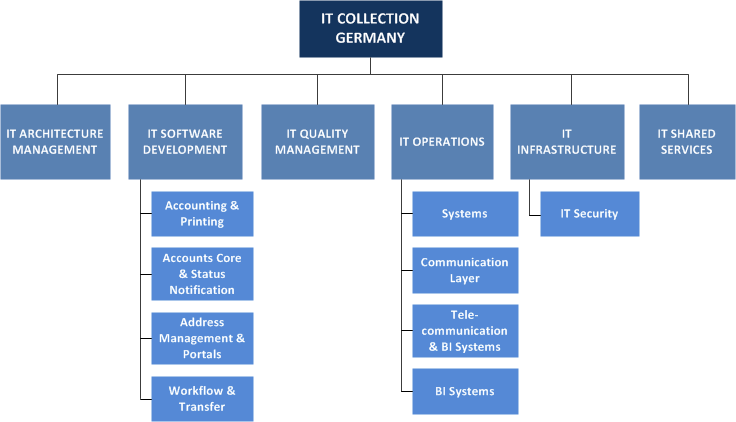
\includegraphics[scale=0.8]{img/IT_Collection_Germany_Organisation.png}
  \caption{Organisationsstruktur IT Collection Germany}
  \caption*{\textbf{Quelle:} Eigene Darstellung}
  \label{fig:organisationsstruktur}
\end{figure}

Weitere Bereiche sind die fachspezifischen Bereiche. Dort wird ebenfalls zwischen Abteilungen und zugehörigen Teams unterschieden. Es gibt Teams, die nur Forderungen eines gewissen Mandanten bearbeiten oder Teams wie das Special Research Team (SRT), das sich um die Ermittlung wichtiger Informationen zum Schuldner kümmert. Jeder Fachbereich hat abhängig von seinem Zuständigkeitsbereich nur auf gewisse Forderungen und Oberflächen im System Zugriff.

\textbf{Inkassosoftware Cosima}

Die digitale Prozessunterstützung wird von der eigens entwickelten Client-Server-Anwen-dung Cosima übernommen. Die Anwendung basiert auf der Programmiersprache Java, daher wurde die grafische Oberfläche komplett mit Java-Swing\footnote{Eine Standardbibliothek der Java-Laufzeitumgebung zur Entwicklung von grafischen Oberflächen} entworfen. Mittlerweile besteht Cosima aus mehreren einzelnen Services und einer Client-Anwendung, die jedem Sachbearbeiter zur Verfügung steht. Cosima wurde ursprünglich am Entwicklerstandort Baden-Baden konzipiert und entwickelt.

Die Inkassosoftware findet in den verschiedensten Fachbereichen und Prozessabläufen anwendung. Cosima wird zum einen als Speichermedium für benötigte Mandanteninformationen, sowie jeglich rechtlich erlaubte und für den Inkassoprozess benötigte Informationen zu Forderungen und Schuldnern verwendet. Zum anderen unterstützt die Software die Sachbearbeiter bei ihrer täglichen Arbeit. 

Durch den ständigen Wandel von Gesetzen, Richtlinien und Anforderungen, muss Cosima durchgehend angepasst und erweitert werden. Darunter leidet auch die Qualität. Mit Blick auf die Performance und die damit verbundene Software-Ergonomie werden daher immer wieder IT getriebene Softwareprojekte ins Leben gerufen, bei denen es darum geht die Softwarequalität zu steigern. So kümmert sich besonders das Qualitätsmanagement darum, dass während des Entwicklungsprozesses gewisse Richtlinien und Normen eingehalten werden. Außerdem werden bestehende Benutzeroberflächen, die den Anforderungen nicht mehr gerecht werden, weil sie unübersichtlich oder ineffizient sind, nach und nach renoviert.

%%%%%%%%%%%%%%%%%%%%%%%%%%%%%%%%%%%%%%%%%%%%%%%%%%%%%%%%%%%%%%%%%%%%%%%%%%%%

\subsection{Ist-Situation und Problemstellung}
Durch zusätzliche Features und Anforderungen ist Cosima mit der Zeit immer weiter gewachsen. Meist bestehen solche Features aus einer erweiterten Datenstruktur und letztendlich einer Veränderung, Anpassung beziehungsweise Erweiterung von Benutzerschnittstellen. Cosima besitzt über achthundert verschiedene Dialoge zur Anzeige und Bearbeitung von Daten. Einer dieser Dialoge ist für die Verwaltung von Schuldnerinformationen zuständig. Genauer gesagt werden dort Informationen zur Lebenssituation, Finanzsituation und dem Vermögen eines Schuldners gespeichert. Die Oberfläche wird mittlerweile für mehr als nur einen Anwendungsfall eingesetzt und besitzt daher einige Bedien- und Eingabeelemente, die für den ursprünglichen Use-Case unrelevant sind. Dadurch, dass der Dialog für mehrere Anwendungsfälle verwendet wird aber nicht jeder Anwendungsfall die kompletten Daten aus dem Dialog benötigt, entsteht ein Overhead\footnote{Daten, die nicht zu den primären Nutzdaten zählen}, der das Arbeiten mit dem Dialog unnötig verkompliziert. Sachbearbeiter finden den Dialog inzwischen sehr unübersichtlich und die Benutzung eher schwerfällig und ineffizient.

Einer dieser Anwendungsfälle (siehe Anhang \ref{sec:ablaufZwangsvollstreckung}) tritt immer dann auf, wenn Schuldner ihre ausstehenden Forderungen nicht begleichen möchten oder nach eigenen Angaben nicht können. In diesen Fällen wird dann eine Zwangsvollstreckung eingeleitet. Dazu wird der Schuldner von einem, durch die \gls{AFS} beauftragten Gerichtsvollzieher, aufgesucht, um einen Vermögensantrag bzw. Vermögensverzeichnis (siehe Beispielformular im Anhang \ref{sec:beispielVermoegensverzeichnisFormular}) zu seiner aktuellen Lebens- und Finanzsituation auszufüllen. Dieser Antrag besitzt einen standardisierten Aufbau und wird, nachdem er vom Schuldner ausgefüllt wurde, an die \gls{AFS} geschickt. Als nächstes wird durch das System automatisch ein Listeneintrag\footnote{Ein Arbeitsauftrag, der für Sachbearbeiter im System erscheint} erstellt, der einem zuständigen Sachbearbeiter zugeteilt wird. Im ersten Arbeitsschritt öffnet der Mitarbeiter das, als PDF vorliegende, Dokument auf einem seiner Monitore. Gleichzeitig öffnet er den Dialog für Schuldnerinformationen auf einem weiteren Monitor. Nach und Nach werden dann die vorliegenden Angaben aus dem Vermögensantrag in den Dialog übernommen und am Ende abgespeichert.

Das Problem speziell in diesem Fall liegt darin, dass der Sachbearbeiter für zwei untereinander folgenden Informationen aus dem Antrag teilweise an mehrere verschiedenen Stellen in dem Dialog springen muss, um diese zu übernehmen. Der Arbeitsablauf wird durch solche Sprünge unterbrochen und der Bearbeiter muss sich häufig neu orientieren. Zudem ist der Dialog mit zunehmender Anzahl an Bedienelementen, auch immer unübersichtlicher geworden. Sachbearbeiter berichten immer wieder von einer zu komplexen und ineffizienten Benutzeroberfläche. Grundsätzlich brauchen auch neue Arbeitskräfte bei der Einarbeitung mit diesem Dialog länger als gewünscht. Der aktuelle Dialog ist in die Jahre gekommen und entspricht nicht mehr den Anforderungen der Verantwortlichen. Aus diesen Gründen sind sich die Beteiligten einig, dass eine Veränderung durchgeführt werden muss.

%%%%%%%%%%%%%%%%%%%%%%%%%%%%%%%%%%%%%%%%%%%%%%%%%%%%%%%%%%%%%%%%%%%%%%%%%%%%

\subsection{Zielsetzung, Forschungsfrage und Hypothesen}
Die Ist-Situation inklusive ihrer Problemstellung, dient als Ansatzpunkt für mein Projektziel, das sich in zwei Unterziele aufteilt. Der erste Teil des Ziels besteht aus der Konzeption und Implementierung eines neuen Dialogs für die Eingabe von Vermögensverzeichnissen bzw. -anträgen. Im zweiten Schritt soll dieser Dialog mit dem bestehenden Dialog für Vermögensverzeichnisse auf Basis einer empirischen Evaluation in den Disziplinen Ergonomie bzw. Effektivität, Effizienz und Benutzerzufriedenheit verglichen werden. Am Ende soll ein neuer Dialog zur Verfügung stehen, der dem Sachbearbeiter eine ergonomische, anwendungsfallorientierte und performante Eingabe von Vermögensverzeichnissen ermöglicht. Dabei soll dieses Projekt als erster Schritt für die Ablösung des alten Dialoges dienen. 

Im Verlauf der Abschlussarbeit gilt es, das zu erreichende Ziel, auch hinsichtlich aufgestellter Hypothesen und Antithesen zu überprüfen. Neben den Thesen gibt es eine zentrale Forschungsfrage, die mit den gewonnen Erkenntnissen und Ergebnissen am Ende der Thesis beantwortet werden soll. Die Hauptfrage mit der sich beschäftigt werden soll lautet: \enquote{Weist der neue Eingabedialog für Vermögensverzeichnisse eine höhere Gebrauchstauglichkeit auf als der alte Dialog?}.

Zusätzlich zu der Forschungsfrage werden drei Hypothesen aufgestellt, die im Ergebnisteil überprüft werden sollen. Die Hypothesen bzw. deren Antithesen dienen später als Hilfe bei der Beantwortung der Forschungsfrage. Die Nullhypothesen werden mit H1\textsubscript{0}, H2\textsubscript{0} und H3\textsubscript{0} deklariert und die entsprechenden Antithesen mit H1\textsubscript{A}, H2\textsubscript{A} und H3\textsubscript{A}. Eine der zu verifizierenden Hypothesen in diesem Kontext heißt H1\textsubscript{0}: \enquote{Wenn der neue Dialog verwendet wird, dann sinkt die durchschnittliche Bearbeitungszeit pro Bearbeitungsvorgang}. Dabei definiert sich ein Bearbeitungsvorgang als Eingabe der Daten eines Vermögensverzeichnisses in die Oberfläche. Eine weitere damit verbundene Hypothese lautet H2\textsubscript{0}: \enquote{Mit dem neuen Dialog sinkt die durchschnittliche Anzahl von Interaktionen pro Bearbeitungsvorgang auf der Oberfläche}. Im Bereich der Ergonomie wird die Hypothese H3\textsubscript{0}: \enquote{Der neue Dialog wird im Gegensatz zum alten Dialog als ergonomischer empfunden} aufgestellt. Zudem werden diese Hypothesen ebenfalls als zu untersuchenden Antithesen umformuliert H1\textsubscript{A}: \enquote{Wenn der neue Dialog verwendet wird, dann stagniert oder steigt die durchschnittliche Bearbeitungszeit pro Bearbeitungsvorgang}, H2\textsubscript{A}: \enquote{Mit dem neuen Dialog steigt die durchschnittliche Anzahl von Interaktionen pro Bearbeitungsvorgang auf der Oberfläche} und H3\textsubscript{A}: \enquote{Der neue Dialog wird im Gegensatz zum alten Dialog als gleich bzw. weniger ergonomisch empfunden}.

%%%%%%%%%%%%%%%%%%%%%%%%%%%%%%%%%%%%%%%%%%%%%%%%%%%%%%%%%%%%%%%%%%%%%%%%%%%%






\section{Grundlagen}

%%%%%%%%%%%%%%%%%%%%%%%%%%%%%%%%%%%%%%%%%%%%%%%%%%%%%%%%%%%%%%%%%%%%%%%%%%%%

\subsection{Eingesetzte Technologien und Programme}
Im Folgenden werden Technologien und Programme vorgestellt, die während des Projektes eingesetzt wurden.

Unter den Technologien, die in dem Projekt Verwendung finden, befindet sich für die programmatischen Implementierungsarbeiten die Programmiersprache Java sowie deren Standardbibliotheken für grafische Benutzeroberflächen. Als integrierte Entwicklungsumgebung wird im Entwicklungsumfeld Eclipse Neon eingesetzt. 

Im Bereich der Datenauswertung und der grafischen Aufbereitung von Daten kommen die Standardprogramme Excel, Word und Visio, als Teil der Microsoft Office Suite, zum Einsatz. 

Für alle datenbankspezifischen Tätigkeiten wird die Datenbanksprache Oracle SQL mit dem Oracle eigens entwickelten Datenbankmanagement Programm SQL-Developer verwendet. Das auf einer grafischen Benutzeroberfläche basierende Tool, ist speziell zur Ausführung von Oracle SQL-Queries entwickelt worden. Mit der eingebetteten Autovervollständigung und Syntax Überprüfung lassen sich relativ einfach und unkompliziert verschachtelte Datenbankabfragen erstellen und ausführen. Die ausgeführten Abfragen werden anschließend innerhalb einer Ausgabekonsole tabellarische dargestellt. Zusätzlich bietet der SQL-Developer eine übersichtliche Möglichkeit Datenbankstrukturen zu verwalten. 

%%%%%%%%%%%%%%%%%%%%%%%%%%%%%%%%%%%%%%%%%%%%%%%%%%%%%%%%%%%%%%%%%%%%%%%%%%%%

\subsection{Software-Ergonomie}
Zunächst soll der Begriff der Software-Ergonomie genauer erläutert werden. Anschließend werden Begriffe, die in einem direktem Zusammenhang mit der Software-Ergonomie stehen, erklärt und abgegrenzt. Darauffolgend werden verschiedene Normen, Richtlinien, Gesetze, Verordnungen und zuletzt sogenannte Usability Heuristiken, die in der Vergangenheit entworfen wurden, vorgestellt.

%%%%%%%%%%%%%%%%%%%%%%%%%%%%%%%%%%%%%%%%%%%%%%%%%%%%%%%%%%%%%%%%%%%%%%%%%%%%

\subsubsection{Begriffsdefinition}
\begin{quote}
    Die Software-Ergonomie hat es sich zur Aufgabe gemacht, die Merkmale benutzer- und aufgebengerechter Software zu erforschen und konstruktive Verfahren sowie Softwareunterstützungen für den Prozeß der Gestaltung von Benutzungsschnittstellen zu entwickeln. Ihr zentrales Anliegen ist die Optimierung des Zusammenspiels aller Komponenten der Arbeitssituation von Computerbenutzern: Mensch, Aufgabe, Technik und organisatorischer Rahmen.\footnote{\cite{Maass1993}}
\end{quote}
Eine relativ allgemeine aber trotzdem sehr treffende und umfassende Definition von Software-Ergonomie, wurde durch die Authorin Dr. Susanne Maaß 1993 veröffentlicht. 

Neben der Beschreibung von Dr. Susanne Maaß, gibt es noch viele weitere Definitionen darunter auch die von Stefano Nocentini, veröffentlicht in einem der Werke von Reinhard Oppermann. Software-Ergonomie ist die \enquote{ability of a software system to interact easily and effectively with the user in order to fulfil his/her needs and expectations}\footnote{\cite[4]{Oppermann1988einfuehrung}}, also die Fähigkeit einer Software einfach und effektiv mit einem Benutzer zu interagieren und dabei dessen Anforderungen und Erwartungen zu erfüllen. Das Ergebnis aus der Software-Ergonomie ist die Usability also die Gebrauchstauglichkeit einer Software. Sie ist besonders dort wichtig, wo Menschen mit Maschinen über Schnittstellen arbeiten\footnote{\cite[vgl.][]{usabilityDe}}. Die Usability ist der Zusammenschluss von Effektivität, Effizienz und Zufriedenheit. Effektivität beschreibt die Erreichung und das Ausmaß von Zielen. Effizienz stellt den Aufwand für die Erledigung des Ziels dar. Die Zufriedenheit spiegelt subjektive Faktoren wie \enquote{joy of use}, \enquote{look and feel} und \enquote{motivation and fun} wider\footnote{\cite[vgl.][]{Holzinger2011human}}. Die Zufriedenheit wird auch als \gls{UX} bezeichnet, die als Erweiterung der Gebrauchstauglichkeit gesehen wird, da sie ästhetische und emotionale Faktoren mit einbezieht\footnote{\cite[vgl.][]{usabilityDe}}. Die Software-Ergonomie gehört neben der Hardware-Ergonomie und Organisations-Ergonomie zu den drei ergonomischen Disziplinen. Auch die Software-Ergonomie selbst lässt sich in drei weitere Bereiche aufteilen: Korrektheits-Ergonomie, Funktionalitäts-Ergonomie und Schnittstellen-Ergonomie\footnote{\cite[vgl.][]{Oppermann1988einfuehrung}}.

%%%%%%%%%%%%%%%%%%%%%%%%%%%%%%%%%%%%%%%%%%%%%%%%%%%%%%%%%%%%%%%%%%%%%%%%%%%%

\subsubsection{Gestaltgesetze}
\label{sec:gestaltgesetze}
In der Vergangenheit wurden durch interdisziplinären Ansätze verschiedene Gestaltgesetze entwickelt, die als Hilfestellung bei der Entwicklung von grafischen Benutzerschnittstellen dienen sollen. Gestalt bedeutet dabei soviel wie die automatische Zusammenfassung bzw. Gruppierung von Objekten\footnote{\cite[vgl.][59]{Dahm2006}}. Bei der Beobachtung von Bildern und Grafiken werden unterbewusst gewisse Muster und Gruppen aus einzelnen Elementen gebildet. Diese Muster und Gruppen lassen sich in einige wichtige Gestaltgesetze abstrahieren, die schon 1923 von drei Forschern beobachtet und niedergeschrieben wurden. Die Gestaltsgesetze können für das Gruppieren und Abgrenzen von Elementen untereinander verwendet werden, um eine höhere Ästhetik bzw. Übersichtlichkeit zu erzielen. Im Folgenden werden exemplarisch drei der wichtigsten und zugleich die drei, für das Projekt, am stärksten berücksichtigten Gestaltgesetze vorgestellt.

\textbf{Gesetz der Ähnlichkeit}

Wie in Abbildung \ref{fig:aehnlichkeit} zu sehen ist, werden ähnliche Objekte zusammengefasst. Für den Betrachter gruppieren sich die grauen und blauen Elementen und er nimmt Spalten wahr.
\begin{figure}[H]
  \centering
  
\includegraphics[scale=1]{img/gesetz_der_Aehnlichkeit.PNG}
  \caption{Ähnliche Objekte werden zusammengefasst.}
    \caption*{\textbf{Quelle:}\footnote{\cite{Dahm2006}}}
  \label{fig:aehnlichkeit}
\end{figure}
Für die Ähnlichkeit sind die Farbe, die Helligkeit, die Form, das Muster und noch weitere Kriterien von Bedeutung\footnote{\cite[vgl.][59f]{Dahm2006}}. Je mehr Kriterien Elemente gemeinsam haben, desto höher ist dessen Ähnlichkeit und desto eher werden Elemente als Gruppe gesehen\footnote{\cite[vgl.][]{HTMLSeminarDe}}.

\textbf{Gesetz der Nähe}

Das Gesetz der Nähe beschreibt die Zusammengehörigkeit von Elementen durch ihre Nähe zueinander.
\begin{figure}[H]
  \centering
  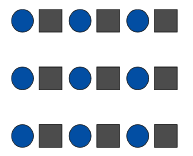
\includegraphics[scale=1]{img/gesetz_der_Naehe.PNG}
  \caption{Abstände zwischen Objekten erzeugen eine Zusammengehörigkeit.}
    \caption*{\textbf{Quelle:}\footnote{\cite{Dahm2006}}}
  \label{fig:naehe}
\end{figure}
In der Abbildung \ref{fig:naehe} ist zu erkennen, dass die Elemente trotz unterschiedlicher Formen und Farben  nicht als Spalten, sondern als Zeilen, wahrgenommen werden. Dieser Effekt resultiert aus dem dominanten Merkmal der Nähe von Objekten. Die Nähe erzielt bei der Anordnung von Elementen einen noch stärkeren Effekt als die Ähnlichkeit\footnote{\cite[vgl.][60]{Dahm2006}}.


\textbf{Gesetz der Vertrautheit}

Das Gesetz der Vertrautheit beschreibt ein Phänomen, bei dem der Betrachter vertraute bzw. bekannte Formen immer wieder erkennt. Dafür sieht er aber nicht mehr die Bestandteile aus denen die Form entstanden ist.\footnote{\cite[vgl.][63f]{Dahm2006}}
\begin{figure}[H]
  \centering
  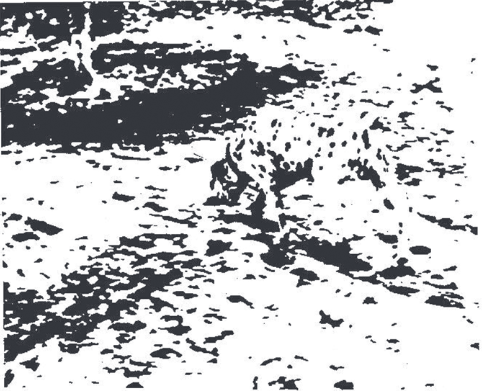
\includegraphics[scale=0.7]{img/gesetz_der_Vertrautheit.PNG}
  \caption{Vertraute Formen bleiben beim Betrachter erhalten.}
  \caption*{\textbf{Quelle:}\footnote{\cite{Dahm2006}}}
  \label{fig:vertrautheit}
\end{figure}
In Abbildung \ref{fig:vertrautheit} sieht der Betrachter auf den ersten Blick viele wahllos verstreute schwarze Flecken auf einem weißen Hintergrund. Wird nun die Erfahrung des Betrachters mit Informationen zu diesem Bild angereichert, wird er zukünftig diese Erfahrungen automatisch immer wieder abrufen. Dabei wird es unmöglich sein, diese Erfahrungen bewusst zu unterdrücken. In der Abbildung ist in der rechten Bildhälfte ein herabschauender Dalmatiner zu sehen. Von vielen Personen wird der Dalmatiner durch bloßes hinschauen nicht wahrgenommen. Sobald der Betrachter einmal den Dalmatiner entdeckt hat, wird er nie wieder nur wahllose Flecken sehen können.\footnote{\cite[vgl.][63f]{Dahm2006}}

%%%%%%%%%%%%%%%%%%%%%%%%%%%%%%%%%%%%%%%%%%%%%%%%%%%%%%%%%%%%%%%%%%%%%%%%%%%%

\subsubsection{Normen und Richtlinien}
\label{sec:normenUndRichtlinien}
Zu der Gestaltung und Anordnung von Elementen, gibt es eine Vielzahl von Normen und Richtlinien, die sich aus verschiedensten Arbeitsgruppen, Institutionen und Gremien entwickelt haben. Ein Grund für ihre Existenz sind die zunehmende Bedeutung von Benutzerschnittstellen und deren Gebrauchstauglichkeit und gleichzeitig auch die steigende Komplexität von Benutzerschnittstellen. Die Normen, also Anweisungen einer höheren Instanz, für das Verhalten bei gewissen Tätigkeiten, Situationen, o.Ä.\footnote{\cite[vgl.][]{duden}}, dienen als Unterstützung für die Entwicklung von einheitlichen und benutzerfreundlichen Benutzerschnittstellen. 

\textbf{Normen}

Einer dieser Software-Ergonomie Normen ist die \gls{EN} \gls{ISO} 9241. Diese wurde in ihrer ersten Auflage 1996 durch das \gls{DIN} veröffentlicht. Seitdem sind die Anforderungen und technischen Möglichkeiten immer weiter gewachsen. In dem Zuge wurde die Norm 2008 in einer überarbeiteten Fassung herausgegeben. Dabei wurden konkretere Beispiele und Empfehlungen vervielfältigt, der Nutzungskontext, der zuvor nur mit dem Blick auf PC'S gerichtet war, erweitert und zusätzlich andere Normen mit einbezogen.\footnote{\cite[vgl.][]{Schneider2008}}

Der Begriff Gebrauchstauglichkeit wird in der Norm 9241-110 mit den drei Merkmalen Effektivität, Effizienz und Zufriedenheit aus der Norm 9241-11 definiert. Zudem wird im Kapitel 6 des Normteils 110 (ehemals Teil 10) die Verbindung der sieben Gestaltungsgrundsätze für ergonomische Benutzerschnittstellen (s. Tabelle \ref{tab:siebenGrundprinzipien}), aus EN ISO 9241-110 und EN ISO 9241-12, zu der Gebrauchstauglichkeit aus EN ISO 9241-11 hergestellt. Denn durch die Anwendung der sieben Grundsätze soll die Gebrauchstauglichkeit unterstützt werden.\footnote{\cite[vgl.][Kap. 6]{ISO9241-110}}

Wie in der Tabelle \ref{tab:siebenGrundprinzipien} zu erkennen ist, wurden die einzelnen Grundprinzipien in ihren Beschreibungen möglichst generisch formuliert. Ein Grund dafür ist, dass die Grundsätze unabhängig vom betrachtenden Softwaresystem angewandt werden sollen. Die Grundsätze können bei der Konzeption, Analyse und Bewertung von Dialogen angewandt werden, sollen aber keine Vorgaben an die Entwicklung von interaktiven Systemen stellen.\footnote{\cite[vgl.][Kap. 4.1]{ISO9241-110}}
\pagebreak
\begin{center}
\begin{longtable}{|p{5.1cm}|p{9.5cm}|} 
\hline
\textbf{Grundprinzip} & \textbf{Beschreibung} \\ \hline
Aufgabenangemessenheit & Ein interaktives System ist aufgabenangemessen, wenn es den Benutzer unterstützt, seine Arbeitsaufgabe zu erledigen, d.h., wenn Funktionalität und Dialog auf den charakteristischen Eigenschaften der Arbeitsaufgabe basieren, anstatt auf der zur Aufgabenerledigung eingesetzten Technologie. \\ \hline
Selbstbeschreibungsfähigkeit & Der Dialog ist in dem Maße selbstbeschreibungsfähig, in dem für den Benutzer zu jeder Zeit offensichtlich ist, in welchem Dialog, an welcher Stelle im Dialog er sich befindet, welche Handlungen unternommen werden können und wie diese ausgeführt werden können. \\ \hline
Erwartungskonformität & Ein Dialog ist erwartungskonform, wenn er den aus dem Nutzungskontext heraus vorhersehbaren Benutzerbelangen sowie allgemein anerkannten Konventionen entspricht. \\ \hline
Lernförderlichkeit & Ein Dialog ist lernförderlich, wenn er den Benutzer beim Erlernen der Nutzung des interaktiven Systems unterstützt und anleitet. \\ \hline
Steuerbarkeit & Ein Dialog ist steuerbar, wenn der Benutzer in der Lage ist, den Dialogablauf zu starten sowie seine Richtung und Geschwindigkeit zu beeinflussen bis das Ziel erreicht ist. \\ \hline
Fehlertoleranz & Ein Dialog ist fehlertolerant, wenn das beabsichtigte Arbeitsergebnis trotz erkennbar fehlerhafter Eingaben entweder mit keinem oder mit minimalem Korrekturaufwand seitens des Benutzers erreicht werden kann. Fehlertoleranz wird mit den Mitteln erreicht: 
\begin{itemize}\itemsep0pt
  \item Fehlererkennung und -vermeidung (Schadensbegrenzung)
  \item Fehlerkorrektur oder
  \item Fehlermanagement, um mit Fehlern umzugehen, die sich ereignen.
\end{itemize} \\ \hline
Individualisierbarkeit & Ein Dialog ist individualisierbar, wenn Benutzer die Mensch-System-Interaktion und die Darstellung von Informationen ändern können, um diese an ihre individuellen Fähigkeiten und Bedürfnisse anzupassen.\\ \hline
\caption{Die sieben Grundprinzipien der Dialoggestaltung in Anlehnung an die ISO 9241-110.}
\label{tab:siebenGrundprinzipien}
\end{longtable}
\end{center}
Bei der konkreten Umsetzung sollten zunächst Merkmale der zukünftigen Benutzer, Arbeitsaufgaben, Arbeitsumgebung aber auch die zur Verfügung stehenden Technologien analysiert werden, um herauszufinden welche dieser Prinzipien im vorliegenden Kontext geeignet sind.\footnote{\cite[vgl.][]{Figl2010}}

Im Abschnitt 12 der ISO Norm 9241 werden die charakteristischen Eigenschaften der Informationsdarstellung, d.h. Klarheit, Unterscheidbarkeit, Kompaktheit, Konsistenz, Erkennbarkeit, Lesbarkeit und Verständlichkeit als unterstützendes Bindeglied für die sieben Grundsätze aus Teil 110 definiert. Insbesondere die Selbstbeschreibungsfähigkeit und Erwartungskonformität einer Benutzerschnittstelle können durch die Eigenschaften der ISO 9241-12 positiv beeinflusst werden. Insgesamt sind die Teile 110, 11 und 12 der ISO Norm 9241 eng miteinander verkettet und können positive aber auch negative Effekte aufeinander ausüben\footnote{\cite[vgl.][Kap. 6]{ISO9241-110}}. Die Wirkungsrichtungen der einzelnen Teile werden in Abbildung \ref{fig:beziehungIsoNormen} noch einmal genauer verdeutlicht.
\begin{figure}[H]
  \centering
  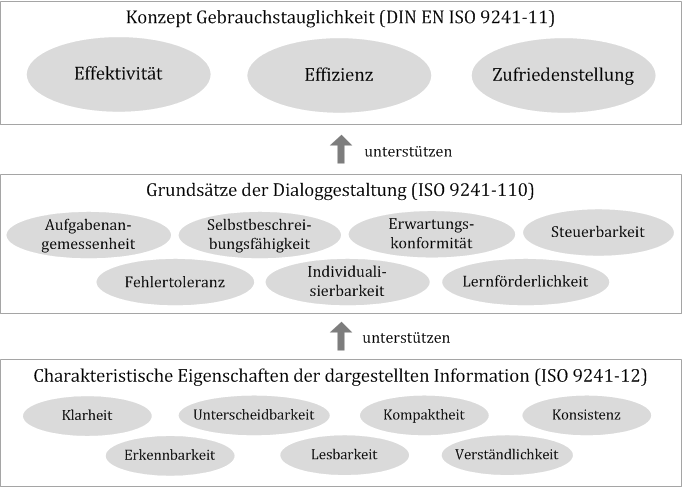
\includegraphics[scale=0.80]{img/Beziehung_ISO9241_ISO9241-11_ISO9241-12.png}
  \caption{Beziehung zwischen ISO 9241, ISO 9241-11 und ISO 9241-12 in Anlehnung an \citep[]{ISO9241-110}.}
  \caption*{\textbf{Quelle:} Eigene Darstellung}
  \label{fig:beziehungIsoNormen}
\end{figure}
Eine weitere Norm im Bereich der Software-Ergonomie, auf die im Abschnitt 3.6 in der ISO 9241-110 Norm verwiesen wird, ist die DIN EN ISO 13407 (Benutzerorientierte Gestaltung interaktiver Systeme). Diese Norm ist als Ergänzung des Teils 110, im Bereich des Projektmanagements und der Vorgehensweisen, anzusehen\footnote{\cite[vgl.][58]{Schneider2008}}.

\textbf{Richtlinien}

Zu den Richtlinien, die man bei der Software-Ergonomie berücksichtigen sollte, gehören auch die Styleguides eines Unternehmens dazu. Dabei wird zwischen internen und externen Richtlinien unterschieden\footnote{\cite[vgl.][74]{Richter2013}}. Das Ziel dieser Styleguides ist es Systeme zu vereinheitlichen, indem gewisse Rahmenbedingungen festgelegt werden\footnote{\cite[vgl.][]{Sarodnick2011}}. Sie enthalten Vorgaben zum Aussehen und Verhalten von Bedienelementen, im jeweiligen Kontext\footnote{\cite[vgl.][72]{Richter2013}}. Jedes Unternehmen sollte gewisse Standards verfolgen, damit eine einheitliche und konsistente Weiterentwicklung und Benutzung der Software gewährleistet ist.

Der Vorteil von Styleguides liegt darin, dass dem Entwickler gewisse Denkprozesse bei der Auseinandersetzung mit Oberflächen durch die Styleguides abgenommen werden. Ebenso dienen sie auch gleichzeitig als eine Art Checkliste für den Entwickler\footnote{\cite[vgl.][214]{Thomaschewski2013}}.

Auf der anderen Seite bringen Styleguides auch per se Probleme mit sich. Beispielsweise deckt die beiliegende Dokumentation nicht alle Funktionen und Ziele ab oder es braucht mehrere Styleguides, die aber untereinander nicht konsistent sind oder die Styleguides sind nicht auf dem aktuellsten Stand. Diese Probleme erzeugen wiederum Schwierigkeiten und Probleme bei der Umsetzung\footnote{\cite[vgl.][215]{Thomaschewski2013}}. Daher sollte darauf geachtet werden, dass die Dokumentationen zu jedem Zeitpunkt aktuell und widerspruchsfrei vorzufinden sind.

%%%%%%%%%%%%%%%%%%%%%%%%%%%%%%%%%%%%%%%%%%%%%%%%%%%%%%%%%%%%%%%%%%%%%%%%%%%%

\subsubsection{Gesetze und Verordnungen}
\label{sec:gesetzeUndVerordnungen}
Neben den Gestaltgesetzen, Normen und Richtlinien, die mit ihren Empfehlungen im Designprozess unterstützen, gibt es Gesetze und Verordnungen die gewisse Vorgaben und Standards fordern. Diese sind darauf bedacht die Arbeitnehmer zu schützen und eine nationale wie auch internationale Vereinheitlichung von IT-Systemen zu fördern. Die \gls{ArbStaettV}, die anstelle der vorherigen Arbeitsschutzverordnung am 3. Dezember 2016 in Kraft getreten ist, ist einer dieser schützenden Gesetze. Die \gls{ArbStaettV} hat als Ziel Beschäftigte in Arbeitsstätten vor Arbeitsunfällen und Berufskrankheiten zu schützen. Das Gesetz enthält Mindestvorgaben an die Arbeitsstätten, die zur Sicherheit und zum Gesundheitsschutz der Beschäftigten eingeführt wurden.\footnote{\cite[vgl.][]{BAuA}}

Ein Zusammenhang des Gesetztes mit dem Thema Ergonomie wird deutlich, wenn man sich den Anlagen Teil 6 des Gesetztes anschaut. Dort lassen sich Maßnahmen und Vorgaben zur Gestaltung von Bildschirmarbeitsplätzen finden. Diese Anforderungen, wie zum Beispiel die angemessene Skalierung von Texten und Grafiken oder auch der ausreichende Kontrast von Texten und Grafiken zum Hintergrund, tragen ebenfalls zu den ergonomischen Gesichtspunkten einer gebrauchstauglichen Benutzerschnittstelle bei.\footnote{\cite[vgl.][Anhang: Kap. 6]{ArbStaettV}}

%%%%%%%%%%%%%%%%%%%%%%%%%%%%%%%%%%%%%%%%%%%%%%%%%%%%%%%%%%%%%%%%%%%%%%%%%%%%

\subsubsection{Heuristiken der Gebrauchstauglichkeit}
\label{sec:heuristikenDerGebrauchstauglichkeit}
Auf dem Gebiet der Usability von Benutzerschnittstellen und der Interaktion mit Schnittstellen, sind die Informatik Professoren Ben Shneidermann und Don Norman und der Usability Berater Dr. Jakob Nielsen, eine renommierte Referenz\footnote{\cite[vgl.][]{Wong2018}}. Ihre Vielzahl an Werken werden gerne als Referenz genutzt und ihre Erkenntnisse im Gebiet der Software-Ergonomie sind durchaus anerkannt. Diese praktikablen Ansätze und Vorgehensweisen für die Evaluation von ergonomischen Benutzerschnittstellen werden Usability Heuristiken genannt. Heuristiken sind Methoden, die auf überlieferten Verhaltensweisen und Erfahrungen basieren und dabei helfen komplexe Probleme zu lösen\footnote{\cite[vgl.][]{Heuristik2018}}. Im folgenden werden 10 Usability Heuristiken von Dr. Jakob Nielsen vorgestellt.
\begin{itemize}
    \item Das System sollte dem Anwender immer wieder den aktuellen Status mitteilen \citep[vgl.][]{Nielsen1995}.
    \item Die Sprache und Ausdrucksweise des Systems sollte zu dem des Anwenders passen. Dazu zählt auch, dass Informationen in realen und logischen Reihenfolgen dargestellt werden \citep[vgl.][]{Nielsen1995}.
    \item Der Anwender sollte die Möglichkeit haben Aktionen zu widerrufen und erneut auszuführen. Bei kritischen Aktionen sollte erst nach einer Bestätigung der Status eines Dialoges gewechselt werden \citep[vgl.][]{Nielsen1995}.
    \item Die Konventionen für Syntax und Semantik sollten systemweit einheitlich eingehalten werden \citep[vgl.][]{Nielsen1995}.
    \item Das System sollte so konzipiert sein, dass es keine Fehlermeldungen zulässt \citep[vgl.][]{Nielsen1995}.
    \item Wichtige Informationen sollte jederzeit im System einsehbar sein. Hilfen zur Handhabung des Systems sollten leicht zugänglich sein \citep[vgl.][]{Nielsen1995}.
    \item Das System sollte sowohl für erfahrene Anwender als auch für unerfahrene Benutzer konzipiert sein \citep[vgl.][]{Nielsen1995}.
    \item Die Dialoge in einem System sollten immer nur wichtige Informationen anzeigen \citep[vgl.][]{Nielsen1995}.
    \item Fehlermeldungen sollten immer in verständlichen Inhalten für den Anwender dargestellt werden und mögliche Lösungswege vorschlagen \citep[vgl.][]{Nielsen1995}.
    \item Das System sollte eine ausreichende System- und Anwenderdokumentation besitzen. Außerdem sollten Informationen einfach in den Dokumentationen zu finden sein \citep[vgl.][]{Nielsen1995}.
\end{itemize}

Um eine all umfassendere Sicht auf mögliche Strategien und Ziele bei der Entwicklung, Analyse und Konzeption von ergonomischen Benutzerschnittstellen zu bekommen, bieten die Ansätze von Dr. Jakob Nielsen eine gute Ergänzung bzw. Erweiterung der Thematik. Eine weitere Auswahl an Usability Heuristiken stellte Ben Shneidermann mit seinen \enquote{8 Golden Rules of Interface Design}\footnote{\cite{Wong2018}} auf. Einige der dort genannten Aspekte decken sich mit den Inhalten der 10 Heuristiken von Dr. Jakob Nielsen.

%%%%%%%%%%%%%%%%%%%%%%%%%%%%%%%%%%%%%%%%%%%%%%%%%%%%%%%%%%%%%%%%%%%%%%%%%%%%

\subsubsection{Nutzen von Software-Ergonomie}
Oftmals ist Unternehmen die Wichtigkeit der Software-Ergonomie zwar bewusst, jedoch schrecken sie zurück, wenn zusätzliche Aufwände im Entwicklungsprozess aufgebracht werden müssen. Diese Kosten und Aufwände erscheinen, verglichen zum erzielten Mehrwert, oftmals für den ersten Moment zu hoch. Langfristig gesehen wird sich jedoch die Software-Ergonomie positiv auf die Produktivität auswirken. Sobald es darum geht Arbeitsabläufe zu optimieren und Zeit zu sparen sind ergonomische Softwaresysteme unabdinglich. Ein gutes Beispiel für die Produktivitätssteigerung durch Software-Ergonomie ist das Service Dialog Center (Call-Center), in dem die Mitarbeiter teilweise durchgehend mit den Software Systemen ihres Unternehmens konfrontiert sind und dessen Produktivität unter anderem davon abhängt, wie benutzerfreundlich bzw. ergonomisch die Software auf sie zugeschnitten ist. Dort können schon jeweils wenige Sekunden Ersparnis im Arbeitsablauf eines einzelnen Mitarbeiters, einen großen Mehrwert insgesamt erzielen.\footnote{\cite[vgl.][19]{Pruemper_Harten2007}}

Die Produktivität setzt auch voraus, dass die Mitarbeiter keinen zu großen Belastungen (physisch und psychisch) ausgesetzt sind. Das heißt sowohl repetitive\footnote{repetitiv = sich wiederholend} Bewegungen der Finger, Hände, Arme und Schultern als auch der Arbeitsablauf und die Arbeitsorganisation sollten möglichst gering bzw. einfach gehalten werden. Zu hohe psychische Belastungen können daraus resultieren, dass zum Beispiel Zeitdruck, ein hoher Konzentrationsaufwand oder zu viele Unterbrechungen in den Arbeitsabläufen auftritt. Diese negativen Effekte gilt es durch eine ergonomische Software möglichst effektiv abzufangen und vorzubeugen.\footnote{\cite[vgl.][19]{Pruemper_Harten2007}}

Auch mit dem Blick auf die laufenden Kosten einer Software können langfristig große Einsparungen erreicht werden. Umso eher sich im Entwicklungsprozess mit dem Thema Software-Ergonomie auseinander gesetzt wird, desto weniger Kosten fallen später für die Erstellung der Dokumentation, die Vorbereitung und Durchführung von Schulungen und die Wartung der Software an.\footnote{\cite[vgl.][19]{Pruemper_Harten2007}}

%%%%%%%%%%%%%%%%%%%%%%%%%%%%%%%%%%%%%%%%%%%%%%%%%%%%%%%%%%%%%%%%%%%%%%%%%%%%

\subsection{Evaluation von Software-Ergonomie}
Die Evaluation im allgemeinen beschäftigt sich mit dem Sammeln und Kombinieren von Daten. Diese Daten dienen zur systematischen Auswertung und Interpretation des Evaluationsgegenstandes (z.B. Programm, Projekt, Produkt, u.a.). Für nachvollziehbare Ergebnisse, ist die Validität und Reliabilität der erhobenen Daten und Vorgehensweisen wichtig.\footnote{\cite[vgl.][7]{Hegner2003}}

%%%%%%%%%%%%%%%%%%%%%%%%%%%%%%%%%%%%%%%%%%%%%%%%%%%%%%%%%%%%%%%%%%%%%%%%%%%%

\subsubsection{Evaluationsziele}

Bei der Evaluation von Software-Ergonomie lassen sich verschiedene Ziele verfolgen. Zum Beispiel kann ein Unternehmen Interesse daran haben Software miteinander zu vergleichen, um herauszufinden welche Software besser auf sie zugeschnitten ist\footnote{\cite[vgl.][]{Gediga2002evaluation}}. In dem Fall wäre die Fragestellung \enquote{Which is better?} die Ausgangslage für die vergleichende Evaluation\footnote{\cite[vgl.][9]{Hegner2003}}. Die bewertende Evaluation ist eine weitere Herangehensweise und stellt die Frage \enquote{How good?}\footnote{\cite[vgl.][9]{Hegner2003}}. Ziel ist es eine Software hinsichtlich gewisser Kriterien und Normen zu bewerten\footnote{\cite[vgl.][]{Gediga2002evaluation}}. Die dritte Möglichkeit ist die analysierende Evaluation also \enquote{Why bad?}\footnote{\cite[vgl.][9]{Hegner2003}}, bei der das Ziel ist, die Schwachstellen eines Systems aufzudecken und Verbesserungsvorschläge aufzustellen\footnote{\cite[vgl.][]{Gediga2002evaluation}}.

%%%%%%%%%%%%%%%%%%%%%%%%%%%%%%%%%%%%%%%%%%%%%%%%%%%%%%%%%%%%%%%%%%%%%%%%%%%%

\subsubsection{Arten der Evaluation}
Bei der Art der Evaluation lässt sich zwischen der formativen Evaluation und der summativen Evaluation unterscheiden.

\textbf{Formative Evaluation}

Bei der formativen Evaluation versucht man mit entsprechenden Methoden möglichst früh im Entwicklungsprozess anzusetzen, um eine hohe Software Qualität und damit auch Ergonomie zu erzielen. Frühzeitige Benutzerbeteiligung und Prototyping helfen dabei die Bedürfnisse der Anwender in der Software abbilden zu können. Die formative Evaluation erhebt sowohl quantitative als auch qualitative Daten. Dabei werden die quantitativen dazu genutzt die Zielerfüllung zu überprüfen. Die qualitativen Daten hingegen werden zur Ableitung von Schwächen und Verbesserungsvorschlägen verwendet. Sie kommen überwiegend in der formativen Evaluation zum Einsatz.\footnote{\cite[vgl.][7]{Hegner2003}}

\textbf{Summative Evaluation}

Zum anderen gibt es die summative Evaluation, die darauf ausgerichtet ist Software miteinander zu vergleichen oder Hypothesen und Erwartungen zu überprüfen. Dazu könnte eine Software zum Beispiel an gewissen Kriterien gemessen werden, die zu Anfang aufgestellt wurden. Die Verfahren zur Erhebung von empirischen Daten stammen überwiegend aus dem quantitativen Bereich, wie zum Beispiel die Befragungsmethode des Fragebogens (siehe Kap. \ref{sec:erhebungsmethoden}).\footnote{\cite[vgl.][8]{Hegner2003}}

%%%%%%%%%%%%%%%%%%%%%%%%%%%%%%%%%%%%%%%%%%%%%%%%%%%%%%%%%%%%%%%%%%%%%%%%%%%%

\subsubsection{Erhebungsmethoden}
\label{sec:erhebungsmethoden}
Bei der Evaluation im Bereich der Software gibt es verschiedene Methodiken und Vorgehensweisen, mit denen sich Daten erheben lassen. Diese erhobenen Daten sind im Evaluationsprozess von Bedeutung. Je nach Ziel, Benutzergruppe, Ort, Art der Informationen und Ressourcen, fällt die Wahl einer Evaluationsmethode unterschiedlich aus\footnote{\cite[vgl.][10]{Hegner2003}} und somit auch die Art der Erhebung. Die Ausrichtung einer Erhebungsmethode lässt sich von objektiv über empirisch und analytisch bis hin zu subjektiv einordnen\footnote{\cite[vgl.][15]{Hegner2003}}.

\textbf{Objektive Methoden}

Bei den objektiven Methoden ist es das Ziel, \enquote{harte} Daten zu erheben und zu bewerten. Diese harten Daten werden durch die bloße Beobachtung des Evaluationsgegenstandes ermittelt. Die Daten liegen in strukturierter Form vor und sind unabhängig von der subjektiven Wahrnehmung der Benutzer. Die objektiven Methoden zielen auf Daten, wie zum Beispiel die Bearbeitungszeit oder Fehlerraten, ab und eigenen sich eher zum Vergleich von zwei Systemen. Jedoch besitzen diese Methoden keinerlei Kontextinformationen und sind somit nicht für die Erarbeitung von Verbesserungsvorschlägen geeignet.\footnote{\cite[vgl.][17]{Hegner2003}}

\textbf{Subjektive Methoden}

Subjektive Methoden versuchen möglichst nah bei den Eindrücken und Erfahrungen der Benutzern anzusetzen. Dabei werden Meinungen und Einschätzungen der Benutzer eingeholt, um den zu evaluierenden Gegenstand zu bewerten. Die erhobenen Daten zählen zu den \enquote{weichen} Daten. Die subjektiven Methoden sind in ihrer Durchführung mit eher geringem Aufwand verbunden, jedoch kann die nachfolgende Auswertung, bei umfangreichen Antworten, sehr zeitintensiv sein.\footnote{\cite[vgl.][18]{Hegner2003}}

Man kann sagen, dass beide Arten von Methoden ihre Vor- und Nachteile besitzen, daher ist es oftmals sinnvoll die Methodiken miteinander zu kombinieren. Dadurch werden Schwächen mancher Methoden durch Stärken anderer ausgeglichen\footnote{\cite[vgl.][261]{Pruemper1997}}. In der Abbildung \ref{fig:erhebungsmethodenObjektivitaetBenutzerbeteiligung} wird noch einmal verdeutlicht welche Erhebungsmethoden es gibt und wie diese im Kontext der Objektivität bzw. Subjektivität und der dazu stehenden Benutzerbeteiligung einzuordnen sind.
\begin{figure}[H]
  \centering
  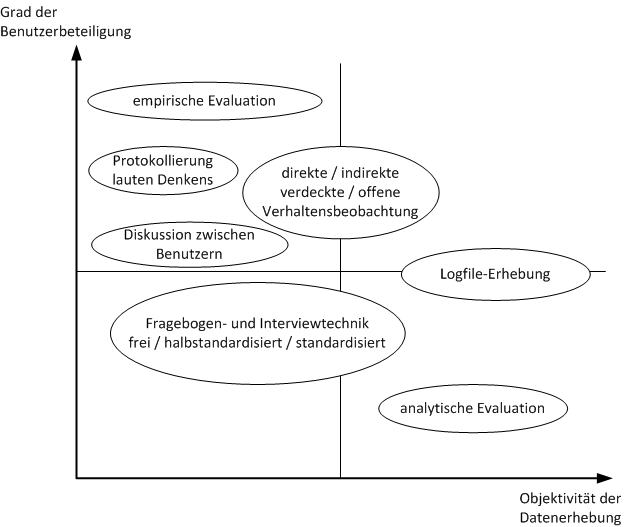
\includegraphics[scale=0.8]{img/Datenerhebungsmethoden_Objektivitaet_Benutzerbeteiligung.png}
  \caption{Vergleich von Erhebungsmethoden aufgrund des Grades der Benutzerbeteiligung und der Objektivität der Methode in Anlehnung an \citep[vgl.][16]{Hegner2003}}
  \caption*{\textbf{Quelle:} Eigene Darstellung}
  \label{fig:erhebungsmethodenObjektivitaetBenutzerbeteiligung}
\end{figure}
Man kann sehen, dass sich die Methoden teilweise nicht genau einer Kategorie zuordnen lassen. Daher wurden zwischen der Subjektivität und der Objektivität noch die Formen der analytischen (leitfadenorientierten) und der empirischen Evaluation eingeführt\footnote{\cite[vgl.][15]{Hegner2003}}.

Im folgenden werden explizit nur die Erhebungsmethoden vorgestellt und eingeordnet, die im Zuge meiner Ausarbeitung zum Einsatz kamen.

\pagebreak
\textbf{Logfile-Erhebung}

Eine Methode zur Erhebung objektiver Daten ist die Logfile-Erhebung. Bei der Methode werden die Daten automatisch durch ein Erfassungssystem erhoben. Interaktionen die Benutzer mit dem System erzeugen werden vollständig aufgezeichnet. Beispielsweise werden Zeiten zwischen Interaktionen oder die Häufigkeit von Maus- und Tastaturanschlägen gemessen\footnote{\cite[vgl.][63]{Hegner2003}}. Diese Methode der Erhebung bietet eine effiziente und kostengünstige Aufzeichnung von Beobachtungsdaten\footnote{\cite[vgl.][Kap. 65.3]{Baur2014}}. Da die Logfile-Erhebung keine Kontextinformationen erfasst und rein objektive Daten wie z.B. Maus- oder Tastaturanschläge aufzeichnet, bietet sich eine Kombination mit einer Befragungsmethode wie z.B. dem Fragebogen an\footnote{\cite[vgl.][17\psq]{Hegner2003}}.

\textbf{Fragebogen}

Eine subjektive jedoch in Teilen auch objektive Methode ist der standardisierte Fragebogen. Hierbei werden von den Benutzern Meinungen, Erfahrungen und Einschätzungen zum untersuchenden Evaluationsgegenstand eingeholt. Das Ergebnis eines Fragebogens kann durch eine Häufigkeitsauswertung von freien und vorgegebenen Antworten ermittelt werden. Je freier eine Frage beantwortet werden darf, umso vielfältiger wird das Antwortenspektrum. Auf der anderen Seite sinkt bei steigender Freiheit die Bereitschaft der Befragten zu antworten und bestenfalls auch konstruktiv zu antworten. Im Bereich der Usability gibt es mehrere standardisierte Fragebögen wie den Questionnarie for User Interaction Satisfaction (QUIS), den IsoMetrics oder den Isonorm 9241/10 Fragebogen, welcher nachfolgend genauer vorgestellt wird.\footnote{\cite[vgl.][Kap. 4.5.1.1]{Hegner2003}}

Der aus dem deutschsprachigen Raum stammende Isonorm 9241/10 Fragebogen, wurde wie auch der IsoMetrics Fragebogen, basierend auf der EN ISO 9241-110 entwickelt. Sein Fragenkatalog unterteilt sich in sieben Kriterien, die äquivalent zu den Gestaltungsgrundsätzen der EN ISO 9241-10 sind. Mit fünf Items pro Kriterium besitzt der Fragebogen insgesamt 35 Items. Jedes der Aussagen wird auf einer 7-stelligen Ratingskala (siehe Abb. \ref{fig:IsonormBewertungsskala}) bewertet, die von sehr negativ (\enquote{$---$}) bis sehr positiv (\enquote{$+++$}) reicht\footnote{\cite[vgl.][Kap. 3.3]{Figl2010}}. 
\begin{figure}[H]
  \centering
  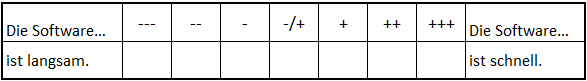
\includegraphics[scale=0.95]{img/Isonorm_Bewertungsskala.PNG}
  \caption{Bewertungsskala des Isonorm 9241/110 Fragebogens.}
  \caption*{\textbf{Quelle:} Eigene Darstellung}
  \label{fig:IsonormBewertungsskala}
\end{figure}
Mit einer etwa 10 minütigen Bearbeitungszeit, eignet sich der Isonorm Fragebogen besonders bei der Frage: \enquote{Entspricht die Software den Kriterien der EN ISO 9241-110 Norm?}. Zudem lässt er sich gut in iterative Softwareprozesse einbringen, indem er für eine schnelle Evaluierung der einzelnen Prototypen eingesetzt wird\footnote{\cite[vgl.][Kap. 3.3]{Figl2010}}.

\textbf{Interview}

Zu den qualitativen Erhebungsmethoden in der empirischen Sozialforschung zählen die Interviews. Diese können aufgrund ihres Grades an Strukturiertheit, der Art des Kontaktaufnahme, der Gruppengröße und dem Autoritätsanspruch des Interviewers in unterschiedlichen Formen vorliegen\footnote{\cite[vgl.][61]{Hegner2003}}. Die Spannweite dabei reicht von sehr offenen Interviews, bei denen weder die Fragen noch die Reihenfolge festgelegt sind, bis hin zu sehr strukturierten Interviews wie dem \enquote{Teacher Relationship Interview}, bei dem Fragen, Nachfragen und deren Reihenfolge vorgegeben werden. Allgemein sind Interviews dann interessant, wenn neue Erkenntnisse oder Meinungen zu einem Thema eingeholt werden sollen. Der Vorteil dabei ist, dass die Befragten Freiräume bekommen, um ihre Meinungen, Sichtweisen und Orientierungen zu äußern\footnote{\cite[vgl.][52\psqq]{Kelle2008}}. Auf der anderen Seite führen Interviews bedeutend höhere Kostenaufwände mit sich, als beispielsweise schriftliche Befragungen\footnote{\cite[vgl.][62\psq]{Hegner2003}}.

%%%%%%%%%%%%%%%%%%%%%%%%%%%%%%%%%%%%%%%%%%%%%%%%%%%%%%%%%%%%%%%%%%%%%%%%%%%%

\subsubsection{Gütekriterien für Erhebungsmethoden}

Die Güte oder auch Qualität einer Erhebungsmethode wird anhand der drei Hauptgütekriterien Objektivität, Validität und Reliabilität bewertet. Darüber hinaus gibt es auch noch weitere Nebengütekriterien (z.B. Normierung, Ökonomie oder Nützlichkeit)\footnote{\cite[vgl.][Kap. 3.5]{Figl2010}} auf die im Folgenden jedoch nicht genauer eingegangen werden soll.

Die Objektivität sagt aus, ob ein Testergebnis unabhängig von der Testperson ist. Bedeutet das verschiedene Personen, die gleichen Testergebnisse erzielen\footnote{\cite[vgl.][Kap. 1]{Himme2007}}. Dieses Kriterium wird, im Fall des Isonorm Fragebogens, durch die standardisiert vorgegebenen Antwortmöglichkeiten und die Auswertungsvorschriften für die Ergebnisse gewährleistet\footnote{\cite[vgl.][Kap. 3.5.1]{Figl2010}}.

Die Validität gibt an, inwiefern ein Messinstrument gültig ist bzw. die benötigte Genauigkeit besitzt. Es wird überprüft, ob das Gemessene, dem entspricht, was gemessen werden soll\footnote{\cite[vgl][Kap. 1]{Himme2007}}. Dabei lässt sich bei der Validität zwischen Inhalts-, Kriteriums und Konstruktvalidität unterscheiden. In allen drei Bereichen zeigt der Isonorm Fragebogen eine ausreichende Erfüllung der Anforderungen\footnote{\cite[vgl.][Kap. 3.5.2]{Figl2010}}.

Als drittes Qualitätsmerkmal wird die Reliabilität herangezogen. Diese beschreibt die Zuverlässigkeit und Stabilität eines Messinstruments. Um eine hohe Zuverlässigkeit bei der Erhebung von Daten zu erreichen, müssen unter anderem gemessene Ergebnisse durch erneutes Messen reproduzierbar sein\footnote{\cite[vgl.][Kap. 1]{Himme2007}}. Der Isonorm Fragebogen weist sowohl eine gute innere Konsistenz als auch eine hohe Retest-Reliabilität auf\footnote{\cite[vgl.][Kap. 3.5.3]{Figl2010}}. Die Logfile-Erhebung weist, durch eine hohe Automatisierung, generell eine höhere Reliabilität als ein Fragebogen auf\footnote{\cite[vgl.][Kap. 65.3]{Baur2014}}.

%%%%%%%%%%%%%%%%%%%%%%%%%%%%%%%%%%%%%%%%%%%%%%%%%%%%%%%%%%%%%%%%%%%%%%%%%%%%

\subsection{Usability-Engineering}
\subsubsection{Vorgehensmodell}
\label{sec:vorgehensmodellUsabilityEngineering}
Usability-Engineering ist ein Vorgehen, das mit Hilfe eines Vorgehensmodell und dazugehörigen Methoden, bei der Entwicklung von benutzerfreundlicher Software unterstützt. Dabei ist ein Vorgehensmodell eine definierte Abfolge von Prozessschritten, die während des Entwicklungsprozesses durchlaufen werden\footnote{\cite[vgl.][7]{Richter2013}}. Generell lässt sich bei Vorgehensmodellen in der Entwicklung zwischen konventionellen und agilen Modellen unterscheiden. Zu den konventionellen oder auch klassischen Ansätzen zählen zum Beispiel das Wasserfallmodell\footnote{\cite[vgl.][27\psqq]{Brandt2008}}. Die klassischen Modelle sind meist einfach zu verstehen aber durch ihre sequenzielle\ Abfolge von Prozessschritten eher unflexibel in der Handhabung.

Agile Vorgehensmodelle, wie zum Beispiel das Spiralmodell oder \gls{XP}, folgen einem iterativen Ansatz. Im Entwicklungsprozess bedeutet das, dass mehrmals gleiche Phasen bzw. Tätigkeiten durchlaufen werden können und keine vordefinierte Reihenfolge eingehalten werden muss\footnote{\cite[vgl.][29\psqq]{Brandt2008}}. Grundsätzlich werden beim Usability-Engineering das Umfeld (Nutzungskontext), die Arbeitsabläufe, geeignete Funktionalitäten und Konzepte zu den grafischen Benutzeroberflächen analysiert und erarbeitet. Dabei hat sich das Usability-Engineering zum Ziel gemacht, komplexe Strukturen zu vereinfachen und eine Lösung zu entwerfen, die genau auf die Anforderungen der Benutzergruppe angepasst ist\footnote{\cite[vgl.][7]{Richter2013}}. Somit bietet sich das Vorgehen gut bei der Entwicklung von grafischen Benutzeroberflächen an, da die Benutzer mit ihren Rückmeldungen ein fester Bestandteil der Entwicklungsphase sind.

Die EN ISO 9241-210 hat das Usability-Engineering als Standardvorgehen bei der Entwicklung von ergonomischer Software etabliert. Das Modell besitzt einen hohen Abstraktionsgrad und lässt sich daher für verschiedene Projekttypen einsetzten\footnote{\cite[vgl.][21]{Ecker2016}}. In der folgenden Abbildung \ref{fig:usabilityEngineeringVorgehensmodell} werden die vier Hauptphasen des Usability-Engineerings nach ISO 9241-210 dargestellt und nachfolgend erläutert.
\begin{figure}[H]
  \centering
  \fbox{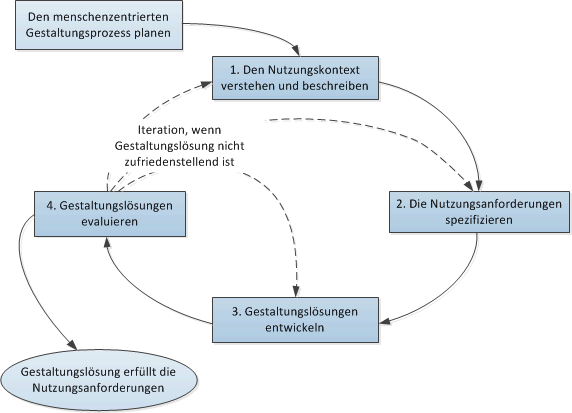
\includegraphics[scale=1]{img/Usability_Engineering_Vorgehensmodell.png}}
  \caption{Usability-Engineering Prozessmodell in Anlehnung an DIN EN ISO 9241-210.}
  \caption*{\textbf{Quelle:} Eigene Darstellung}
  \label{fig:usabilityEngineeringVorgehensmodell}
\end{figure}
\begin{enumerate}
    \item In der ersten Phase des Software Projektes geht es darum, den Nutzungskontext (siehe Kap. 4.4.2) möglichst voll umfassend zu verstehen und zu beschreiben. Zum Nutzungskontext gehören die betroffenen Benutzergruppen mit deren Tätigkeiten und Arbeitsabläufen und die Arbeitsumgebung selbst. Die benötigten Informationen lassen sich mit Hilfe von Erhebungsmethoden (siehe Kap. 4.3.3) wie z.B. Fragebögen oder persönlichen Interviews eruieren\footnote{\cite[vgl.][28\psq]{Ecker2016}}.
    \item In der zweiten Phase des Modells werden die Anforderungen der betroffenen Benutzergruppen analysiert und dokumentiert. Dazu gehört, dass sich der Projektleiter mit den Benutzern und deren Sichtweise auseinander setzt und die Anforderungen zusammen erarbeitet werden\footnote{\cite[vgl.][30\psq]{Ecker2016}}.
    \item Im dritten Prozessschritt werden die definierten Anforderungen in Form von Prototypen oder Mock-ups\footnote{Ein Mock-up ist eine oftmals zu präsentationszwecken grafisch modellierte Attrappe eines Produkts.} ausgearbeitet. In der Phase werden Entwürfe sowohl von der Ablaufsteuerung als auch vom Oberflächendesign erstellt. Die Ablaufsteuerung beinhaltet die wechselseitige Interaktion zwischen Benutzer und Software. Diese Abläufe werden in geeignete Schnittstellen oder Prozessdiagramme abgebildet. Der zweite Teil der Entwicklung besteht aus dem Entwurf der Schnittstelle. Dazu gehört, dass die Interaktionsart (Maus, Tastatur, etc.) mit der Schnittstelle festgelegt wird und dem entsprechend geeignete Bedienelemente ausgewählt und ergonomisch angeordnet werden\footnote{\cite[vgl.][33\psq]{Ecker2016}}.
    \item Im vierten Schritt werden die Gestaltungslösungen aus dem vorherigen Schritt evaluiert. Die Benutzer bewerten die entworfenen Mock-ups, Skizzen oder die fertig implementierte Schnittstelle, um Mängel oder Fehler frühzeitig zu erkennen. Für die Bewertung der Gestaltungslösungen sind Benutzungstests, Fragebögen oder Fokusgruppen\footnote{Eine Art der Gruppendiskussion, bei der moderierte und leitfadenorientierte Fragen diskutiert werden.} mögliche Herangehensweisen. Sollte keiner der Gestaltungslösungen die Nutzungsanforderungen ausreichend erfüllen, so können iterativ vorherige Phasen durchlaufen werden\footnote{\cite[vgl.][34\psq]{Ecker2016}}. Hingegen kann der Entwicklungsprozess bei befriedigender Lösung beendet und die finale Gestaltungslösung ausgerollt werden.
\end{enumerate}

\subsubsection{Analysemethoden}
\label{sec:analysemethoden}
Während des Entwicklungsprozesses gibt es mehrere Techniken mit denen die Gestaltungslösungen analysiert und evaluiert werden können. Unter anderem lassen sich auch die in Kapitel \ref{sec:erhebungsmethoden} vorgestellten Methoden der Befragung mittels Fragebogen oder das Interview anwenden. 

Als weitere Möglichkeit gibt es die Einbeziehung von Experten. Dazu zählt die Methode der heuristischen Evaluation, bei der Gestaltungslösungen anhand aufgestellter Empfehlungen, Normen und Gesetze (siehe Kap. \ref{sec:gestaltgesetze}, \ref{sec:normenUndRichtlinien}, \ref{sec:gesetzeUndVerordnungen} und \ref{sec:heuristikenDerGebrauchstauglichkeit}) bewertet werden. Diese Methode vernachlässigt jedoch die Benutzerbedürfnisse und eignet sich daher eher als ergänzende Methode.\footnote{\cite[vgl.][249]{Nielsen1990}}

Eine weitere benutzerbezogene Methode ist \enquote{Thinking Aloud}. Bei dieser Methode werden wenige Benutzer mit Video und Ton aufgenommen und sollen ihre Gedanken und Probleme während der Bearbeitung von gezielten Aufgabenstellungen äußern. Dadurch sollen Schwachstellen und Probleme beim Umgang mit dem System hervorgehen.\footnote{\cite[vgl.][51]{Hegner2003}}

%%%%%%%%%%%%%%%%%%%%%%%%%%%%%%%%%%%%%%%%%%%%%%%%%%%%%%%%%%%%%%%%%%%%%%%%%%%%

\subsubsection{Nutzungskontext}
Der Nutzungskontext muss im Zuge der zweiten Phase aus dem Vorgehensmodell nach ISO 9241-210 analysiert werden. Der Nutzungskontext setzt sich aus den betroffenen Benutzergruppen, den umliegenden Arbeitsabläufen und dem technischen Umfeld zusammen. Diese Bestandteile sollen im Folgenden genauer erläutert werden.

\textbf{Benutzergruppen}

Einen Teil der Kontextanalyse beinhaltet die Erhebung von Merkmale der Benutzer. Zu den Merkmalen, die durchaus einen Einfluss auf die Entwicklung des interaktiven Systems nehmen können, gehören Kenntnisse, Fertigkeiten, Erfahrungen, Ausbildung, Übungsgrad, physische Merkmale und motorische und sensorische Fähigkeiten\footnote{\cite[vgl.][28]{Ecker2016}}. Die unterschiedlichen Ausprägungen der Benutzer (insofern diese gegeben sind), sollten ebenso mit in den Entwicklungsprozess einfließen.

\textbf{Arbeitsabläufe}

Ebenso spielen für den Entwurf der Benutzerschnittstelle die Ausprägungen der Arbeitsabläufe eine Rolle. Typischerweise sollte neben dem Erfassen der Tätigkeiten und ihrem Zusammenspiel auch die Dauer und Häufigkeit betrachtet werden\footnote{\cite[vgl.][28]{Ecker2016}}.

\textbf{Technisches Umfeld}

Zu Erhebung des technischen Umfelds, lässt sich generell zwischen der Software und der Hardware unterscheiden. Die Software manifestiert sich zum Beispiel im Betriebssystem der Benutzer, dass durchaus Unterschiede aufweisen kann. Hingegen werden zur Hardware jegliche Hilfsmittel am Arbeitsplatz wie Monitore, Drucker oder Taschenrechner gezählt und aufgenommen.\footnote{\cite[vgl.][28]{Ecker2016}}

%%%%%%%%%%%%%%%%%%%%%%%%%%%%%%%%%%%%%%%%%%%%%%%%%%%%%%%%%%%%%%%%%%%%%%%%%%%%

\subsection{Statistische Datenanalyse}
Damit für spätere Auswertungen und Analysen der erhobenen Daten die benutzten Methoden mit denen Daten normalisiert, statistisch bewertet und für grafische Darstellungen aufbereitet werden, klar und verständlich sind werden im Folgenden die Grundbegriffe und weiterreichende Methoden der Statistik, die im Rahmen der Thesis zum Einsatz kommen, vorgestellt und erklärt.

%%%%%%%%%%%%%%%%%%%%%%%%%%%%%%%%%%%%%%%%%%%%%%%%%%%%%%%%%%%%%%%%%%%%%%%%%%%%

\subsubsection{Bereiche der Statistik}
In der Statistik unterscheidet man zwischen drei grundlegenden Aufgabengebieten. Zum einen die deskriptive Statistik, die es sich zur Aufgabe macht Daten komprimiert entweder beschreibend oder grafisch aufzubereiten. Diese Art der Aufbereitung wird häufig zu repräsentativen Zwecken eingesetzt. Dabei kommen verschiedene Diagramme und Tabellen zum Einsatz, die dazu dienen zuvor berechnete Durchschnittsgrößen und Kennzahlen der Merkmale und ihrer Ausprägungen darzustellen. Ein zusätzlich wichtiger Aufgabenbereich der deskriptiven Statistik ist die Datenvalidierung. Durch die deskriptive Aufbereitung der Daten lassen sich Fehler leicht aufdecken und gegeben falls beheben. Somit wird der Aufwand für nachträgliche Korrekturen gemindert.\footnote{\cite[vgl.][10\psq]{Statistik2016}}

Ein weiterer Teilbereich der Statistik ist die explorative Datenanalyse. Sie bietet Methoden mit denen sich Strukturen und Besonderheiten in den Daten aufdecken lassen. Das führt oft dazu, dass neue Hypothesen und Fragestellungen hinzu kommen. Daher wird das explorative Vorgehen immer dann verwendet, wenn die Ausgangslage bzw. Fragestellung noch nicht eindeutig ist. Die Exploration wird als Ergänzung zu der Deskription von Daten angesehen.\footnote{\cite[vgl.][11\psq]{Statistik2016}}

Die induktive Statistik ergänzt den dritten Bereich der Statistik. Dort wird über die erhobenen Daten hinweg, mittels Wahrscheinlichkeitstheorie und stochastischer Methoden, Aussagen und Folgerungen geschlossen. Um aussagekräftige Ergebnisse in der Statistik zu erzielen, wird eine klar definierte und sorgfältig strukturierte Versuchsplanung für alle drei Teilgebiet benötigt.\footnote{\cite[vgl.][12]{Statistik2016}}

%%%%%%%%%%%%%%%%%%%%%%%%%%%%%%%%%%%%%%%%%%%%%%%%%%%%%%%%%%%%%%%%%%%%%%%%%%%%

\subsubsection{Grundbegriffe}
\textbf{Grundgesamtheit und Stichprobe}

Immer wenn es in der Statistik um die Analyse von Daten geht, bei denen die Menge von Bedeutung sind, fallen in diesem Zusammenhang Begriffe wie Grundgesamtheit oder Stichprobe. Die Grundgesamtheit hängt von der betrachteten Einheit ab, über die statistische Aussagen getroffen werden sollen und beschreibt die mögliche Menge dieser Einheit\footnote{\cite[vgl.][13]{Statistik2016}}. Als Beispiel kann eine Schule genommen werden, auf die insgesamt 400 Schüler und Schülerinnen gehen, von denen 250 Jungen und der Rest Mädchen sind. Sollte man auswerten wollen wie viele Schüler Mädchen bzw. Jungen sind, dann besteht die vorliegenden Grundgesamtheit, auf der die statistische Betrachtung basiert, aus allen 400 Schüler und Schülerinnen der Schule.

Da die Einbeziehung der Gesamtheit typischerweise nicht möglich ist, wird die Erhebung bzw. Analyse auf gewisse Kriterien und somit auf einen Teil der Grundgesamtheit eingeschränkt. In dem Fall wird von einer Teilgesamtheit oder Stichprobe gesprochen\footnote{\cite[vgl.][13]{Statistik2016}}. Bezogen auf das obige Beispiel, wäre eine mögliche Fragestellung: \enquote{Wie viele der Jungen kommen im Durchschnitt täglich zu spät zum Unterrichtsbeginn?}, so würde sich die untersuchende Stichprobe aus allen Jungen der Schule zusammensetzen.

\textbf{Statistische Einheit, Merkmal und Merkmalsausprägung}

Wird erneut das Beispiel mit der Schule und den Schülern betrachtet, dann ist die statistische Einheit in diesem Kontext ein einzelner Schüler. Sollte zum Beispiel die Anzahl der Fenster in der Schule ermitteln werden wollen, dann ist die zu untersuchende statistische Einheit beziehungsweise der Merkmalsträger das Fenster.\footnote{\cite[vgl.][13]{Statistik2016}}

Die Eigenschaften einer Einheit wird Merkmal genannt. Mögliche Merkmale, die bei einer Analyse von Schülern untersucht werden können sind Körpergröße, Augenfarbe, Haarfarbe oder Geschlecht. Merkmale können verschiedene Merkmalsausprägungen annehmen. Es kann zwischen qualitativen und quantitativen Ausprägungen unterschieden werden. Beispielsweise ist die Körpergröße ein Merkmal mit quantitativen Ausprägungen, in dem Fall sind alle natürlichen Zahlen größer null möglich. Eine qualitatives Merkmal hingegen ist beispielsweise das Geschlecht, das nur zwei Ausprägungen annehmen kann entweder Mann oder Frau.\footnote{\cite[vgl.][13\psqq]{Statistik2016}}

Grundlegend wird bei Merkmalen und ihren Ausprägungen zwischen drei verschiedenen Skalen zum Messen der Merkmale und ihren Ausprägungen unterschieden. Die Nominalskala stellt das niedrigste Skalenniveau der drei Skalen dar und wird zur Klassifizierung und Darstellung von qualitativen Merkmalsausprägungen verwendet. Merkmale, die dieser Skala angehören, können lediglich gezählt und in der Häufigkeit ihrer Ausprägungen dargestellt werden.\footnote{\cite[vgl.][15\psqq]{Statistik2016}}

Das nächst höhere Skalenniveau wird durch die Ordinalskala abgebildet. Beispielsweise gehören Schulnoten (Ausprägungen: sehr gut, gut, befriedigend, ausreichend, mangelhaft und ungenügend) zur Ordinalskala, die neben den Anwendungsgebieten der Nominalskala auch zum Vergleichen von Ausprägungen genutzt werden kann.\footnote{\cite[vgl.][15\psqq]{Statistik2016}}

Die Intervallskala besitzt nicht nur das höchste Skalenniveau, sondern ist auch am vielfältigsten bei der Berechnung von Lageparametern. Diese werden im nächsten Abschnitt genauer erläutert. Die Intervallskala kann neben dem Vergleichen von Merkmalsausprägungen, auch einen numerischen Unterschied zwischen zwei Ausprägungen ermitteln.\footnote{\cite[vgl.][15\psqq]{Statistik2016}}

%%%%%%%%%%%%%%%%%%%%%%%%%%%%%%%%%%%%%%%%%%%%%%%%%%%%%%%%%%%%%%%%%%%%%%%%%%%%

\subsubsection{Lageparameter}
Lageparameter werden in der deskriptiven Statistik zum Beschreiben eines Mittelpunktes innerhalb einer Verteilung\footnote{Die Verteilung steht für die relative bzw. absolute Häufigkeit von Merkmalsausprägungen.} genutzt\footnote{\cite[vgl.][49]{Statistik2016}}. Im folgenden wird auf die als Lageparameter zählenden Größen Modus, Median und arithmetisches Mittel genauer eingegangen.

Als ersten Lageparameter betrachten wir den Modus, der angibt welche Merkmalsausprägung in einer Verteilung am häufigsten vorkommt\footnote{\cite[vgl.][53]{Statistik2016}}. Als Beispiel nehmen wir eine Befragung bei der eine Stichprobe von 500 Probanden nach ihrer Lieblingsjahreszeit befragt werden. Das Ergebnis der Erhebung ist:
\begin{center}
\begin{tabular}{r|c|c|c|c} 
\textbf{Jahreszeit} & Frühling & Sommer & Herbst & Winter \\ \hline
\textbf{Anzahl Probanden} & 110 & 205 & 85 & 110\\
\end{tabular}
\end{center}
Um anschließend den Modus zu bestimmen, wird das Merkmal mit den meisten Merkmalsausprägungen gesucht. In diesem Fall ist das mit 205 der Sommer.

Im nächsten Schritt wollen wir anhand eines Beispiels den Median berechnen. Da der Median nur auf Ordinalskalen oder Intervallskalen angewandt werden kann, ist das vorherige Beispiel nicht für den Median geeignet\footnote{\cite[vgl.][52]{Statistik2016}}. Das vorliegende Beispiel ist lediglich nominal skaliert.
Um ein Beispiel für den Median zu finden, betrachten wir das Alter von 10 zufällig ausgewählten Probanden, die im ersten Semester Biologie studieren. Die Stichprobe sieht wie folgt aus:
\begin{center}
\begin{tabular}{r|c|c|c|c|c|c|c|c|c|c} 
\textbf{Rang} & 1 & 2 & 3 & 4 & 5 & 6 & 7 & 8 & 9 & 10 \\ \hline
\textbf{Alter} & 20 & 20 & 22 & 23 & 23 & 23 & 25 & 25 & 25 & 26\\
\end{tabular}
\end{center}
Wie sich aus der Tabelle ablesen lässt gibt es 2 x 20, 1 x 21, 3 x 23, 3 x 25 und 1 x 26 als Alter der befragten Probanden. Zur Bestimmung des Medians werden die erhobenen Daten nach ihrer Größe geordnet (ist in der obigen Grafik schon geschehen). Danach wird der mittlere Wert in der Reihe ermittelt\footnote{\cite[vgl.][52\psq]{Statistik2016}}. In diesem Beispiel gibt es zwei mittlere Werte, da die Anzahl $N$ der befragten Probanden gerade ist. Bei geraden Stichprobenumfängen werden die beiden mittleren Merkmalsausprägungen addiert und anschließend durch zwei dividiert, um den Median zu erhalten\footnote{\cite[vgl.][53]{Statistik2016}}. Die konkrete Rechnung dazu sieht folgendermaßen aus: $Median = \frac{23 + 23}{2} = 23$.

Der letzte Lageparameter, der immer dann angewendet werden kann wenn eine Intervallskala vorliegt, ist das arithmetische Mittel. Das arithmetische Mittel, auch bekannt als Mittelwert, gibt den Durchschnittlichen Wert aus einer Datenmenge mit $N$ Merkmalsausprägungen an. Der Mittelwert $\bar{x}$ ergibt sich aus der Summe aller Merkmalsausprägungen geteilt durch die Anzahl $N$ Werte\footnote{\cite[vgl.][49\psq]{Statistik2016}}. Für das obige Beispiel, wird der Mittelwert wie folgt berechnet: \\
$Mittelwert = \frac{\sum \limits_{i=1}^N X_i}{N} = \frac{20\,+\,20\,+\,22\,+\,23\,+\,23\,+\,23\,+\,25\,+\,25\,+\,25\,+\,26}{10} = 23,2 Jahre$. Die Berechnung hat ergeben, dass die Erstsemester Biologie Studenten im Schnitt 23,2 Jahre alt sind.

%%%%%%%%%%%%%%%%%%%%%%%%%%%%%%%%%%%%%%%%%%%%%%%%%%%%%%%%%%%%%%%%%%%%%%%%%%%%

\subsubsection{Dispersionsparameter}
Die nächste Sektion beschäftigt sich mit den Dispersionsparametern. Diese werden verwendet, wenn es darum geht ein Maß für die Streuung von Messwerten, um ein Zentrum zu ermitteln. Zu den bekanntesten Dispersionsparametern gehören unter anderem die Spannweite, die Varianz und die Standardabweichung.

\textbf{Spannweite}

Die Spannweite ist die Differenz zwischen dem größten (Maximum) und dem kleinsten (Minimum) Wert einer Messreihe. Dazu wird das Minimum vom Maximum subtrahiert\footnote{\cite[vgl.][62]{Statistik2016}}. Die Spannweite liefert einen schnellen Überblick über die Bandbreite der Werte\footnote{\cite[vgl.][38]{Kronthaler2016}}. Dazu eine Beispielrechnung mit der zuletzt aufgestellten Messreihe: $Spannweite = 26 - 20 = 6$. Auf den Kontext bezogen bedeutet das Ergebnis, dass der Altersunterschied zwischen dem jüngsten und dem ältesten Student der Untersuchung 6 Jahre beträgt.

\textbf{Varianz}

Wenn es in der Datenauswertung darum geht herauszufinden, wie weit die Messwerte durchschnittlich von dem arithmetischen Mittel abweichen, wird die Varianz berechnet. Die Varianz ist ein Maß für die Streuung von Messwerten um den Mittelwert. Für die Varianz wird in der empirischen Sozialforschung und auch für die nachfolgenden Rechnungen der Platzhalter $s^2$ verwendet. Die Berechnung startet damit, dass die quadrierten Abweichungen der einzelnen Messwerte, vom Mittelwert, aufsummiert werden. Anschließend wird die Summe durch die Anzahl der Messwerte dividiert. In der induktiven Statistik wird es bei größeren Datenmengen bevorzugt die Summe anschließend durch $n-1$ Werte zu dividieren\footnote{\cite[vgl.][65]{Statistik2016}}. Das Quadrat der Abweichung wird aus dem Grund verwendet, dass negative und positive Abweichungen, die aus der Differenz von $Messwert\:x$ und $Mittelwert\:\bar{x} $ entstehen, sich nicht gegenseitig aufheben und das Ergebnis verfälschen\footnote{\cite[vgl.][65]{Statistik2016}}. Die entsprechende Rechnung zum obigen Beispiel: \\
$s^2 = \frac{1}{n - 1} \sum \limits_{i=1}^n (x_i\,-\,\bar{x})^2 = \frac{1}{9}[ (20\,-\,23,3)\:+\:(20\,-\,23,2)\:+\:...\:+\:(26\,-\,23,2)]= 4,4$. 

Das Ergebnis von 4,4 ist nun ein Maß, das die Streuung um den Mittelpunkt angibt. Da für das Endergebnis alle Abweichungen zuerst quadriert wurden, besitzt das Ergebnis durch sein Quadrat eine andere Maßeinheit als die einzelnen Abweichungen\footnote{\cite[vgl.][65]{Statistik2016}}.

\textbf{Standardabweichung}

Um dem Problem, der geänderten Maßeinheit, aus dem Weg zu gehen, gibt es die Standardabweichung $s$, die häufiger in der Statistik eingesetzt wird. Im Gegensatz zu der Varianz wird für das Endergebnis der Standardabweichung, die ermittelte Summe aller quadrierten Abweichungen mit der Quadratwurzel bereinigt. Durch diesen Schritt besitzt das Ergebnis die gleiche Maßeinheit, wie die einzelnen Abweichungen\footnote{\cite[vgl.][65]{Statistik2016}}. Bedeutet im Klartext, dass die Berechnung der Standardabweichung der der Varianz bis auf die Quadratwurzel am Ende gleicht. Somit berechnet sich $s$ für das Beispiel aus der Wurzel von $s^2$. Die Rechnung dazu sieht wie folgt aus: $s = \sqrt{s^2} = \sqrt{4,4} = 2,1$. Interessant wird dieser Parameter, wenn z.B. Intervalle in Zusammenhang mit dem arithmetischen Mitteln angeben werden sollen. Es ist darauf zu achten, dass eine Normalverteilung vorliegt\footnote{\cite[vgl.][67]{Statistik2016}}. Im Folgenden wird dies anhand der Messreihe zu den Erstsemester Biologie Studenten verdeutlicht. Die Intervallen sehen folgendermaßen aus:
\begin{compactitem}
    \item in $\bar{x} \pm s^2$ liegen ca. 70\% aller Daten,
    \item in $\bar{x} \pm 2s^2$ liegen 100\% aller Daten. 
\end{compactitem}
Sollte man Intervalle innerhalb einer nicht normalverteilten Verteilung angeben wollen, eignen sich Box-Plots besser\footnote{\cite[vgl.][67]{Statistik2016}}.

%%%%%%%%%%%%%%%%%%%%%%%%%%%%%%%%%%%%%%%%%%%%%%%%%%%%%%%%%%%%%%%%%%%%%%%%%%%%

\subsection{Kosten-Nutzen-Analyse}
Die Kosten-Nutzen-Analyse \enquote{[...] stellt das wohl bekannteste wirtschaftlichkeitsanalytische Verfahren für den öffentlichen Sektor dar.}\footnote{\cite[vgl.][1]{Hanusch2011}}. Mit Hilfe des Verfahrens kann durch den Vergleich von Kosten und Nutzen eine objektive Aussage über die Wirtschaftlichkeit eines Projektvorhabens getroffen werden. Einerseits werden die Kostenpunkte eines Projektes identifiziert und quantifiziert. Andererseits werden jegliche zu erwartende Effizienzpotential, die aus dem Projektvorhaben resultieren, betrachtet und für einen Vergleich, wenn möglich, monetarisiert. Die \gls{KNA} ist für verschiedenste Personen eines Projektes interessant. Zum Beispiel ist Auftraggebern und Investoren daran gelegen, dass sich das Projekt und die damit entstehenden Kosten nach einer gewissen Zeit amortisiert. Dazu gehört auch ein positives Ergebnis. Gerade in der Planungsphase eines Projekts können Projektbeteiligte mit Hilfe der \gls{KNA} die positiven und negativen Effekte besser abschätzen und so gezielter und effektiver planen und agieren\footnote{\cite[vgl.][]{Hanusch2011}}. Im Folgenden wird auf Grund des Projektumfangs meiner Bachelor Thesis nur von einer minimalistischen Form der \gls{KNA} Gebrauch gemacht. In der späteren Analyse werden bewusst einige Kosten und Nutzen, die entweder nicht klar identifizierbar sind oder wenn erfassbar dann nur in Verbindung mit übermäßigem Aufwand, vernachlässigt. 

Ein Bestandteil der \gls{KNA}, der im oberen Teil schon kurz erwähnt wurde, ist der Amortisationszeitpunkt des zu überprüfenden Projektes, also der Zeitpunkt an dem die Summe der Kosten und der Nutzen gleich null sind. Dieser Zeitpunkt wird auch als Break-Even-Point bezeichnet. Umso näher der Break-Even-Point am Startzeitpunkt des Projekts liegt, desto höher ist dessen Wirtschaftlichkeit einzuschätzen\footnote{\cite[vgl.][]{Hanusch2011}}.

Ein weitere Begriff der im Zusammenhang mit der \gls{KNA} häufig fällt ist das Effizienzpotential. Dies sagt aus, dass der Nutzen eines Projekts ein gewisses Potential besitzt. Jedoch wird dieser Nutzen relativiert, da er in Wirklichkeit noch nicht realisiert wurde und sich durch die Veränderung von Einflussfaktoren zukünftig noch ändern kann.



\section{Entwicklung der neuen Benutzeroberfläche für Vermögensauskünfte}
Eine Hauptaufgabe dieses Projekts ist der Entwurf und die Implementierung einer neuen grafischen Benutzerschnittstelle für die Eingabe von Vermögensverzeichnissen. Diese neue Benutzeroberlfäche soll später die bestehende Eingabeschnittstelle für Vermögensverzeichnisse ablösen. Die neue Eingabemaske soll sich an den Gestaltungsgesetzen, Normen, Verordnungen und Usability Heuristiken, die in den Kapiteln 4.2.2, 4.2.3, 4.2.4 und 4.2.5 vorgestellt wurden, orientieren und die darin enthaltenen Empfehlungen und Prinzipien berücksichtigen. Ebenso erfolgt der Entwicklungsprozess in Anlehnung an das Vorgehensmodell aus Kapitel 4.4. 

Für die initiale Projektvorstellung meiner Bachelor Thesis, wurden im Vorhinein bereits mehrere fachlich und technisch visierte Ansprechpartner mit einbezogen. Während des Entwicklungsprozesses wurden mehrere Gespräche sowohl mit den fachlichen Anforderungsstellern als auch mit den technischen Beteiligten geführt, um die Anforderungen für den neuen Dialog möglichst genau zu definieren.

%%%%%%%%%%%%%%%%%%%%%%%%%%%%%%%%%%%%%%%%%%%%%%%%%%%%%%%%%%%%%%%%%%%%%%%%%%%%

\subsection{Vorgehensmodell für den Entwicklungsprozess}

Zunächst wird das Vorgehensmodell nach ISO 9241-210 an den zeitlichen Rahmen und den Inhalt meines Projektes angepasst. Zu den Anforderungen an die neue Benutzeroberfläche gehören eine möglichst benutzerfreundlich und individuell auf die Benutzer und deren Arbeitsabläufe Abstimmung. Dafür eignet sich das Usability-Engineering als agiles Modell gut. Insbesondere da eine möglichst benutzerorientierte Aufnahme der Anforderungen und Wünsche erfolgen soll. Zudem soll auch ein iteratives Testvorgehen angewandt werden. Das heißt, dass nach jeder entwickelten Gestaltungslösung Benutzungstests von zwei bis drei Testern durchgeführt werden. Die Prototypen werden auf einer separaten Entwicklungsumgebung getestet. Bei den Tests prüfen die Tester den Prototypen auf fachliche und technische Fehler, damit die Wahrscheinlichkeit für schwerwiegende Systemfehler (Systemabsturz, Speicherprobleme o.Ä.) möglichst gering gehalten wird. Die Sachbearbeiter sollen nämlich beim anschließenden Produktivtest reibungslos Arbeiten können. Systemfehler würden sich in den erhobenen Daten widerspiegeln und schlimmsten falls zu Auswertungsfehlern bzw. einem größeren Aufwand für die Fehlerbehebung führen.

Solange die Gestaltungslösungen die Erwartungen und Anforderungen nicht erfüllen kann iterativ in vorherige Phasen gesprungen werden. Sobald ein finaler Entwicklungsstand vorliegt, wird dieser in die produktiv Umgebung ausgerollt, damit anschließend die Evaluation inklusive empirischer Erhebung, zum neuen Dialog, stattfinden kann.

%%%%%%%%%%%%%%%%%%%%%%%%%%%%%%%%%%%%%%%%%%%%%%%%%%%%%%%%%%%%%%%%%%%%%%%%%%%%

\subsection{Aufnahme des Ist-Zustands}
Die Aufnahme des Ist-Zustands ist mit den ersten beiden Phasen des ISO 9241-210 Vorgehensmodell zu vergleichen. Dazu gehört die Erhebung des Nutzungskontextes (Benutzergruppen, Arbeitsabläufe und technisches Umfeld) und der Anforderungen. Da man sich in dem Projekt dazu entschieden hat, eine bestehende Eingabeoberfläche durch eine komplett neue auszutauschen, eignet sich der bestehende Dialog gut als Grundlage für die Anforderungsanalyse. Die Beurteilung von Schwächen und Stärken der aktuellen Benutzerschnittstelle hilft dabei gezielte Anforderungen für den neuen Dialog zu schaffen.

%%%%%%%%%%%%%%%%%%%%%%%%%%%%%%%%%%%%%%%%%%%%%%%%%%%%%%%%%%%%%%%%%%%%%%%%%%%%

\subsubsection{Benutzergruppen}
\label{sec:benutzergruppen}
Zunächst werden die Benutzergruppen und -typen, die später mit der neuen Schnittstelle interagieren, genauer analysiert. Mit Hilfe eines Fragebogens werden Alter, Geschlecht, wöchentlich durchschnittliche Nutzungsdauer von Computern allgemein sowie die der Eingabeoberfläche für Vermögensverzeichnisse, der Probanden, ermittelt. Dazu wurde eine Umfrage an 83 zufällig ausgewählte Probanden (siehe auch Kapitel \ref{sec:empirischeErhebung}) geschickt, um Daten zu ihrem Profil anzugeben. Das durchschnittliche Benutzerprofil wurde auf der Basis von 37 Rückmeldungen aufgestellt und ist in Abbildung \ref{fig:durchschnittlichesBenutzerprofil} abgebildet. 

Die Abteilung wurde aufgrund der vielen unterschiedlichen Ausprägungen im durchschnittlichen Benutzerprofil nicht berücksichtigt. Da es sich bei dem Geschlecht nur um ein nominal skaliertes Merkmal handelt, wurde als Referenzwert der Modalwert ermittelt. Die anderen drei Merkmale sind alle metrisch (gehören zur Kardinalskala), daher konnten die Referenzwerte mit Hilfe des arithmetischen Mittels berechnet werden.
\begin{figure}[H]
  \centering
  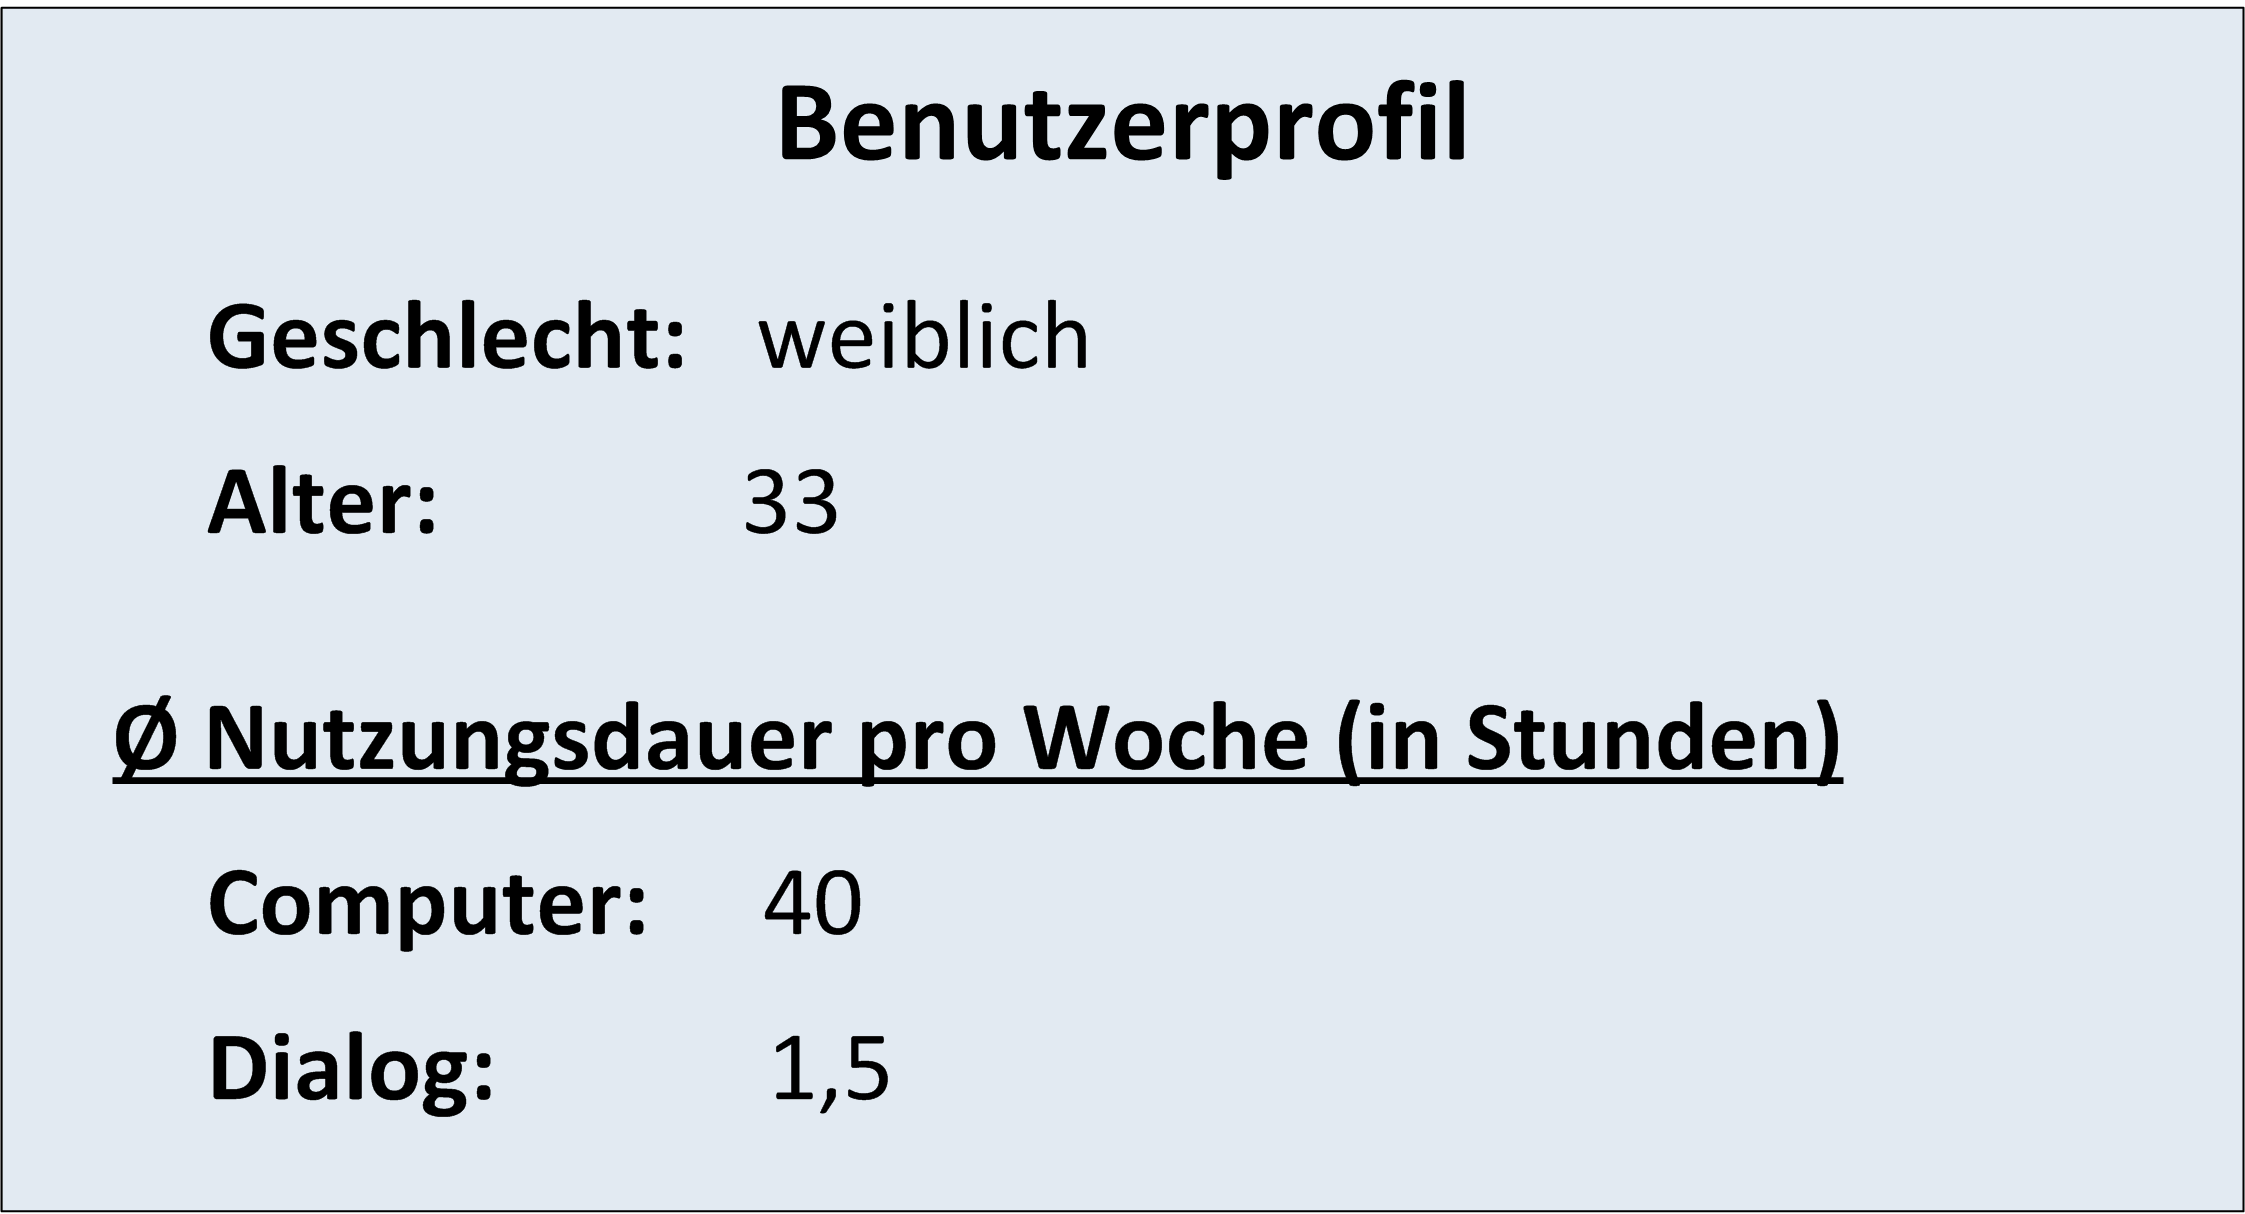
\includegraphics[width=250px]{img/durchschnittliches_Benutzerprofil.png}
  \caption{Typisches Benutzerprofil in der schriftlichen Sachbearbeitung.}
  \caption*{\textbf{Quelle:} Eigene Darstellung}
  \label{fig:durchschnittlichesBenutzerprofil}
\end{figure}
Es lässt sich feststellen, dass sich größtenteils Frauen in der Sachbearbeitung befinden. Zudem ist das durchschnittliche Alter der Benutzer auf rund 35 Jahre zu schätzen. Trotzdem sollte darauf Rücksicht genommen werden, dass eine relativ großer Altersunterschied vorliegt. Die Benutzergruppe setzt sich sowohl aus sehr jungen, als auch aus kurz vor der Rente stehenden Sachbearbeitern zusammen. Dies kann besonders bei der Erfahrung wie auch bei der Lernfähigkeit und Lernbereitschaft zu Diskrepanzen führen.

Betrachtet man die durchschnittliche Nutzungsdauer des Computers von 37,17 Stunden, so ist zu erkennen, dass die Sachbearbeiter großenteils mit dem PC arbeiten und daher mit dem generellen System vertraut sein sollten. Anders sieht es bei Nutzung des Eingabedialogs für Vermögensverzeichnisse aus. Durchschnittlich arbeiten die Benutzer 1,68 Stunden mit dem Dialog. Jedoch herrschen hier relativ große Unterschiede bei der Nutzungsdauer, die durch die unterschiedlichen Mandanten und Aufgabenbereiche der Teams zu begründen sind. Manche Teams müssen sehr häufig den Anwendungsfall \enquote{Eingabe eines Vermögensantrags} behandeln andere nur eher selten. Daher ist davon auszugehen, das auch die Effizienz bei der Benutzung, auf unterschiedlichen Niveaus sein wird. Dies sollte man bei der Evaluation und Datenauswertung im Anschluss ebenfalls berücksichtigen.

%%%%%%%%%%%%%%%%%%%%%%%%%%%%%%%%%%%%%%%%%%%%%%%%%%%%%%%%%%%%%%%%%%%%%%%%%%%%

\subsubsection{Arbeitsabläufe und Tätigkeiten}
Die Arbeitsabläufe wurden mit Hilfe eines persönlichen Interviews und einer Analyse der bestehenden Schnittstelle entworfen und modelliert. Dabei wurde zum einen der Ablauf einer  Zwangsvollstreckung im Ganzen dargestellt (siehe Anhang \ref{sec:ablaufZwangsvollstreckung}) und zum anderen der Arbeitsprozess eines einzelnen Mitarbeiters bei der Eingabe des Vermögensverzeichnisses in das System.

%%%%%%%%%%%%%%%%%%%%%%%%%%%%%%%%%%%%%%%%%%%%%%%%%%%%%%%%%%%%%%%%%%%%%%%%%%%%

\subsubsection{Technisches Umfeld}
Für die Aufnahme des technischen Umfelds wurde sich mit den Beteiligten des Projekts für ein offenes Interview (siehe Kap. 4.3.3) entschieden. Dabei ist herausgekommen, dass alle Sachbearbeiter standardmäßig mit zwei Monitoren und dem Betriebssystem Windows ausgestattet sind. Darüber hinaus stehen den Sachbearbeitern jeweils Maus und Tastatur als weitere Peripherie zur Verfügung. Hilfsmittel wie Drucker sind verteilt vorhanden, werden aber für den vorliegenden Anwendungsfall nicht benötigt, da das Vermögensverzeichnis Dokument in digitaler Form vorliegt. Die weitere Ausstattung für einen Sachbearbeiter sieht einen eigenen Arbeitsplatz vor, der sich je nach Team und Abteilung unterscheiden kann. Typischerweise befinden sich Trennwände zwischen den einzelnen Arbeitsplätzen, um gerade in Großraumbüros die Akustik und Arbeitsatmosphäre zu verbessern. Zusammengefasst ist die Ausstattung und das Umfeld der Sachbearbeiter stark standardisiert und bietet damit für Jeden eine ähnliche Ausgangslage bei der Bearbeitung.

%%%%%%%%%%%%%%%%%%%%%%%%%%%%%%%%%%%%%%%%%%%%%%%%%%%%%%%%%%%%%%%%%%%%%%%%%%%%

\subsubsection{Anforderungsanalyse}
Zunächst wurde in einem initialen Termin darüber gesprochen welche grundsätzlichen Veränderungen die neue Oberfläche im Gegensatz zu der bestehenden Maske mit sich bringen soll. Dafür wurde gemeinsam mit den Beteiligten des Projekts der aktuelle Ist-Zustand der Oberfläche aufgenommen. Die Benutzeroberfläche in Abbildung \ref{fig:aktuellerDialog} ist aktuell produktiv im Einsatz. Diese wurde analysiert und es wurden sowohl negative als auch positive Aspekte aufgegriffen und entsprechende Design Anforderungen für die neue Oberfläche herausgearbeitet.
\begin{figure}[H]
  \centering
  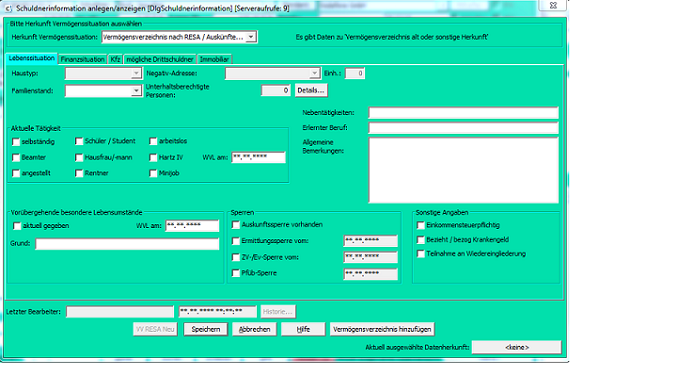
\includegraphics[scale=1]{img/aktueller_Dialog.PNG}
  \caption{Aktueller Dialog für die Eingabe von Vermögensverzeichnissen.}
  \caption*{\textbf{Quelle:} Vermögensverzeichnis Dialog der IFM}
  \label{fig:aktuellerDialog}
\end{figure}
Als Ergebnis stellten sich drei grundlegende Gestaltungsziele heraus. Zu diesen Zielen gehören eine übersichtlichere Anordnung der Bedienelemente, eine reduzierte Auswahl an Bedienelementen mit der Prämisse das die benötigen Elemente zur Verfügung stehen und eine an das Vermögensverzeichnis angelehnte Struktur der Informationen. Zudem wurde für den Entwurf des Prototypen entschieden, dass die Datenstruktur vorerst bestehen bleibt. Benötigte Änderungen am Datenbankmodell sollen erst in einem nachfolgenden Projekt umgesetzt werden. Daraufhin wurde zusammen mit dem zuständigen Fachbereich definiert, welche Bedienelemente in der aktuellen Oberfläche nicht benötigt werden und für die neue Oberfläche somit wegfallen können.

Mit dieser Ausgangssituation an Zielen und ersten spezifischen Anforderungen wird der erste fertig programmierte Prototyp für die Oberfläche entworfen. Dieser wird den Beteiligten dann in einem weiteren Termin präsentiert und anschließend auf einer Testumgebung zur Verfügung gestellt.

%%%%%%%%%%%%%%%%%%%%%%%%%%%%%%%%%%%%%%%%%%%%%%%%%%%%%%%%%%%%%%%%%%%%%%%%%%%%

\subsection{Erarbeitung der Gestaltungslösung}
Im folgenden wird genauer auf den Entwurfsprozess inklusive der Analysemethoden (siehe Kap. \ref{sec:analysemethoden}) eingegangen. Dieser Teil des Entwicklungsprozesses ist mit den Phasen drei und vier aus dem ISO 9241-210 Vorgehensmodell (siehe Kap. 4.4.1) zu vergleichen. Das nachfolgende Vorgehen orientiert sich ebenfalls an dem iterativen Ansatz, bei dem besonderes die Phasen zwei, drei und vier mehrmals durchlaufen wurden, bis die fertige Lösung bereit stand. Die Gestaltungslösungen wurden dabei mit Hilfe von Interviews und heuristischen Evaluationen bewertet und evaluiert.

\textbf{Erster Prototyp}

Der erste Prototyp wurde aufgrund der Anforderungen bewusst nur auf die benötigten Bedienelemente reduziert und sollte mit seiner Formular nahen Struktur einen klaren Fortschritt im Bereich der Übersichtlichkeit verzeichnen. Ebenfalls ist speziell durch die Berücksichtigung der Gestaltgesetze zur Ähnlichkeit und Nähe von Objekten eine klarere Unterteilung von Bedienelementgruppen entstanden. Dies hat die positive Folge das thematisch bzw. strukturell, durch das Formular, nah beieinander liegende Informationen deutlicher werden. Ebenso wurde auf einheitlich, verständlich und präzise formulierte Fehler- und Hinweismeldungen Wert gelegt. Auch hier kamen wieder die Empfehlungen der ISO Norm 9241-110 und die Heuristiken von Jakob Nielsen zu Gute. Durch die Vorgaben der Styleguides musste zudem auf eine entsprechende Dimensionierung von Elementen, so wie auf uneingeschränkte Vergrößerung der Anzeige geachtet werden.

Durch den zweiten Termin in dem der erste Prototyp präsentiert und anschließend evaluiert wurde, konnten die Beteiligten erstmals Eindrücke zu der neuen Oberfläche gewinnen. Zudem konnten erste Benutzungstest auf einer Entwicklungsumgebung durchgeführt werden. Aus der Präsentationsrunde sowie den Benutzungstests gingen überwiegend positive Rückmeldungen zu dem ersten Entwurf hervor. Jedoch war die Auswahl sowie Platzierung gewisser Bedienelemente noch nicht vollständig zufriedenstellend. 

Aufgrund der festgestellten Mängel wurde erneut in die Anforderungsspezifikation gesprungen, um die Anforderungsliste zu verfeinern und mit konkreten Verbesserungsvorschlägen zu bestücken. Diese erweiterten Anforderungen sollten anschließend in einem zweiten Prototypen umgesetzt werden.

\textbf{Finale Version}

Mit Abschluss des ersten Prototypen und der erweiterten Anforderungsliste die aus der Analyse der Stärken und Schwächen resultierte, wurde ein weiterer Prototyp konzipiert. Der in Abbildung \ref{fig:neuerDialog} zu sehende Prototyp ist in drei Sektionen gegliedert, die durch die Verwendung von Rahmenlinien hervorgehoben werden. 
\begin{figure}[H]
  \centering
  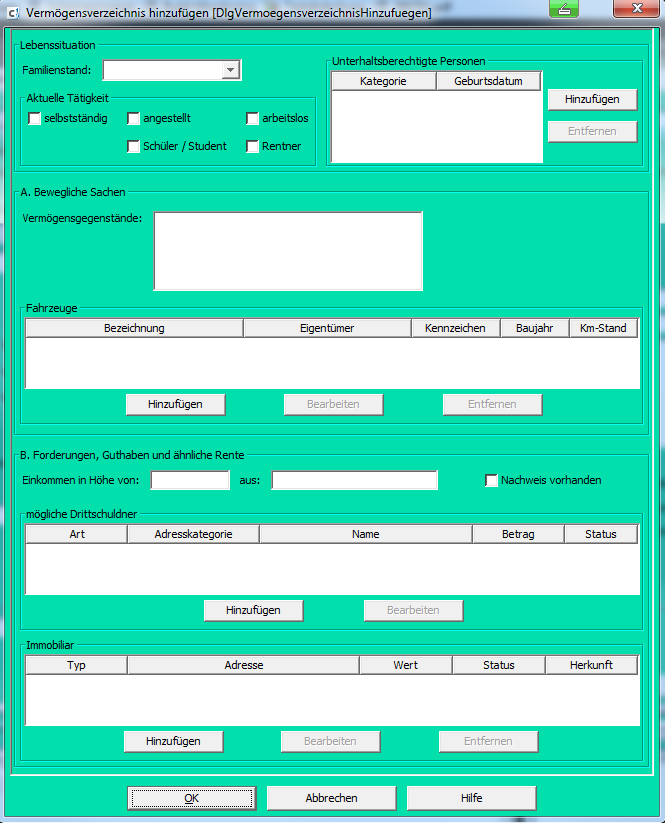
\includegraphics[scale=0.85]{img/neuer_Dialog.PNG}
  \caption{neuer Dialog für die Eingabe von Vermögensverzeichnissen.}
    \caption*{\textbf{Quelle:} Eigene Darstellung}
  \label{fig:neuerDialog}
\end{figure}
Die erste Sektion beinhaltet Informationen zur allgemeinen Lebenssituation eines Schuldners, darunter zum Beispiel der Familienstand oder auch die Art der Tätigkeit. Ein weiteres Unterziel für die neue Oberfläche ist es die Bezeichnungen von Eingabfeldern, Dropdownlisten, Buttons und Checkboxen soweit es geht beizubehalten. Der Nutzen daraus soll später durch eine schnellere Gewöhnung an die neue Oberfläche ersichtlich werden. Durch gleichnamige Felderbezeichnungen werden die Sachbearbeiter an alte bekannte Strukturen, die sie bereits kennen, erinnert und brauchen dadurch bestenfalls weniger Einarbeitungszeit.

Die zweite Sektion des Dialogs visualisiert alle beweglichen Daten. Die Formulierung \enquote{bewegliche Daten} wurde aus dem standardisierten Formular übernommen und enthält Daten zu Vermögensgegenständen und Fahrzeugen der Schuldner. Eine grundlegende Veränderungen wurde bei der Eingabe von Fahrzeugen vorgenommen. Die Informationen zum Fahrzeug wurden zuvor in einzelnen Textfeldern (Bezeichnung, Eigentümer, Kennzeichen u.a.) eingetragen. Diese Textfelder standen aber nur einmal zur Verfügung. Sobald mehr als ein Fahrzeug hinterlegt wurde, mussten die Informationen in einem freien Textfeld \enquote{weitere Fahrzeuge} \ref{fig:fahrzeugTab} eingetragen werden. Diese Lösung war zum einen unschön, da es eine inkonsistente Eingabe der Daten gab und zum anderen auch fehleranfällig, weil einzutragende Informationen schneller vergessen wurden.
\begin{figure}[H]
  \centering
  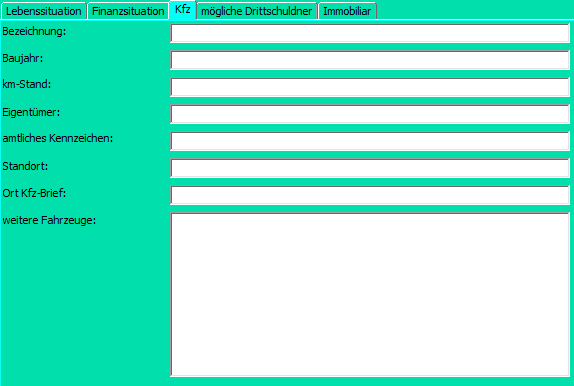
\includegraphics[scale=0.9]{img/FahrzeugTab.PNG}
  \caption{Eingabemaske für Fahrzeuge in der alten Oberfläche.}
    \caption*{\textbf{Quelle:} Vermögensverzeichnis Dialog der IFM}
  \label{fig:fahrzeugTab}
\end{figure}
Der neue Dialog sieht es nun vor jedes Fahrzeug über einen separaten Dialog, der sich über die Schaltfläche \enquote{Hinzufügen} (siehe Abb. \ref{fig:neuerDialog}) öffnen lässt, anzulegen. Die Eingabestruktur ist identisch zu der des alten Dialogs (siehe Abb. \ref{fig:fahrzeugTab}), jedoch werden die Informationen, unabhängig von der Anzahl angelegter Fahrzeuge, in getrennten Feldern hinterlegt. Dadurch entsteht der positive Effekt, dass die Sachbearbeiter sich nicht mehr an unterschiedliche Eingabestrukturen anpassen müssen. Dazu kommt, dass die Daten in gleicher und dadurch auch in vergleichbarer Form gespeichert werden. Der Eingabedialog prüft zudem, ob valide Werte eingegeben wurden und verringert somit die Fehlerquote.
\begin{figure}[H]
  \centering
  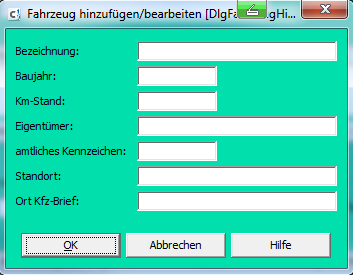
\includegraphics[scale=0.9]{img/FahrzeugAnlegenBearbeiten_Dialog.PNG}
  \caption{neuer Dialog für die Eingabe von Fahrzeugen.}
    \caption*{\textbf{Quelle:} Eigene Darstellung}
  \label{fig:fahrzeugAnlegenBearbeitenDialog}
\end{figure}
Durch die Tabelle \enquote{Fahrzeug} (vgl. \ref{fig:neuerDialog}) bekommt der Sachbearbeiter schnell einen Überblick über alle angelegten Fahrzeuge. Diese lassen sich auch nach der Anlage ohne großen Aufwand noch bearbeiten oder auch wieder löschen. Die neue Lösung verhindert inkonsistente und falsche Daten. Zudem werden Informationen bei der Eingabe, aufgrund der vorgegebenen Eingabestruktur, nicht so schnell vergessen. Dies folgt auch dem Grundsatz \enquote{Recognition rather than recall} von Jakob Nielsen.

Die letzte Sektion \enquote{B. Forderungen, Guthaben und ähnliche Rente} beinhaltet Informationen über das Einkommen des Schuldners, über mögliche Drittschuldner und über Immobiliar. Durch die Berücksichtigung von Empfehlungen zur Aufgabenangemessenheit (vgl. ISO 9241-110 Kap. \ref{sec:normenUndRichtlinien}) und zu einem minimalistischen Design (vgl. Jakob Nielsen Kap. \ref{sec:heuristikenDerGebrauchstauglichkeit}) konnten hier einige Informationen, im Vergleich zum vorherigen Dialog, entfallen. Im vorherigen Dialog wurden die Informationen in drei getrennten Reitern dargestellt. Dies hatte den Nachteil, dass der Benutzer häufig zwischen den Reitern wechseln musste. Zusätzlich wurden noch eine handvoll weiterer Informationen neben dran angezeigt, die überflüssig waren und das Erscheinungsbild unübersichtlicher gemacht haben. Die neue Oberfläche stellt nur die nötigsten Informationen dar und wirkt damit viel aufgeräumter und übersichtlicher und ist der Aufgabenstellung angepasst.

Grundsätzlich wurde sich bei der Gestaltung des neuen Dialogs an interne (Style)-Richtlinien der IFM gehalten. Darunter fällt, dass es Schaltflächen wie \enquote{OK} zum Bestätigen bzw. Speichern, \enquote{Abbrechen} zum Schließen ohne Speichern und \enquote{Hilfe} zum Öffnen einer internen Dokumentation gibt. Durch die Einhaltung der Standards wird zugleich dem Ziel der Erwartungskonformität aus der ISO 9241-110 Norm  zu gearbeitet. Eine weiterer Richtlinie der IFM besagt, dass Eingabefelder, Comboboxen und Buttons vorgegebene Abmessungen in der Höhe besitzen und Dialoge auch bei 125\% Anzeigevergrößerung ohne Fehler oder Einschränkungen angezeigt werden. Die Vergrößerung der Anzeige, soll Sachbearbeitern mit eingeschränktem Sehvermögen das Arbeiten erleichtern.

Mit dem Abschluss der Entwicklungsphase geht eine finale Gestaltungslösung als neuer Vermögensverzeichnis Dialog produktiv. Dieser soll für den weiteren Verlauf des Projekts genutzt werden. Dazu soll als nächster Schritt eine vergleichende Evaluation zwischen dem alten und dem neuen Dialog, auf der Basis empirischer Daten, durchgeführt werden.

%%%%%%%%%%%%%%%%%%%%%%%%%%%%%%%%%%%%%%%%%%%%%%%%%%%%%%%%%%%%%%%%%%%%%%%%%%%%



\section{Evaluation}
Als nächstes soll die Methodik der Evaluation (siehe Kap. 4.3) angewandt werden. Dazu sollen zunächst die Ziele und der Aufbau der Evaluation definiert werden. Da es sich hierbei um eine empirische Evaluation handelt, werden Daten mittels geeigneter Methoden erhoben. Diese Methoden werden nachfolgend ausgewählt und genauer beschrieben.

%%%%%%%%%%%%%%%%%%%%%%%%%%%%%%%%%%%%%%%%%%%%%%%%%%%%%%%%%%%%%%%%%%%%%%%%%%%%

\subsection{Ziel und Aufbau}
Ziel dieser Evaluation ist es, zwei Benutzerschnittstellen hinsichtlich ihrer Effizienz und Ergonomie zu vergleichen. Dabei sind der neu entworfene Dialog aus dem vorherigen Abschnitt \enquote{Erarbeitung der Gestaltungslösung} (siehe Abb. \ref{fig:neuerDialog}), der bereits konzipiert und implementiert wurde und der aktuell im produktiven Einsatz genutzte Dialog für Vermögensverzeichnisse (siehe Abb. \ref{fig:aktuellerDialog}) Gegenstand des Vergleichs. Das Ziel der Evaluation ist bewusst an die Forschungsfrage angelehnt, denn die Evaluation soll später zur Beantwortung bzw. Überprüfung der Forschungsfrage sowie der Hypothesen benutzt werden.

Der Aufbau der Evaluation gliedert sich in vier Phasen. Die erste Phase beschäftigt sich mit generellen Planungstätigkeiten, zu denen auch die Definition des Ziels sowie der Untersuchungsgegenstände zählt. In der darauf folgenden Phase wird die Stichprobe und die Erhebungsmethoden und Messinstrumente für die Erhebung ausgewählt. Anschließend werden in der dritten Phase die Erhebungsmethoden auf die Stichprobe angewandt. In der letzten Phase werden dann in Kapitel \ref{sec:ergebnisseUndDiskussion} alle Datensätze und Erkenntnisse ausgewertet. Schließlich wird mit Hilfe der Evaluationsergebnisse die Hypothesen überprüft und die Forschungsfrage beantwortet.

%%%%%%%%%%%%%%%%%%%%%%%%%%%%%%%%%%%%%%%%%%%%%%%%%%%%%%%%%%%%%%%%%%%%%%%%%%%%

\subsection{Empirische Erhebung}
\label{sec:empirischeErhebung}
Zunächst sollen geeignet Verfahren und eine repräsentative Stichprobe für die Datenerhebung bestimmt werden. Diese werden dann im zweiten Schritt angewandt.

%%%%%%%%%%%%%%%%%%%%%%%%%%%%%%%%%%%%%%%%%%%%%%%%%%%%%%%%%%%%%%%%%%%%%%%%%%%%

\subsubsection{Auswahl der Stichprobe}
Damit im nächsten Schritt eine Auswahl der Stichprobe geschehen kann, muss zu aller erst definiert werden welche und bestenfalls wie viele Personen die Gesamtheit darstellen. Da es sich bei der Evaluation, um die Bewertung der Benutzerschnittstelle für Vermögensauskünfte handelt, zählen alle Personen zur Gesamtheit, dessen tägliche Arbeit mit dem Anwendungsfall \enquote{Eingabe eines Vermögensverzeichnisses} zu tun hat. Das heißt jeder Sachbearbeiter der getrieben durch seine Aufgaben, die Oberfläche für Vermögensauskünfte, zur Eingabe eines neuen Vermögensverzeichnisses benutzt ist potentieller Teil der Grundgesamtheit. In Zahlen ausgedrückt sind dies mehrere hundert Personen. Genaue Zahlen sind sehr schwierig zu ermitteln, daher wird für nachfolgende Aussagen und Rechnungen von einer gerundeten Grundgesamtheit von etwa 550 Personen ausgegangen.

Bei der Auswahl der Stichprobe wird auf eine Kombination der bewussten Auswahl und der Zufallsziehung gesetzt. Es liegt keine vollständig zufällige Stichprobe vor, da bereits ein Benutzerprofil in Kapitel \ref{sec:benutzergruppen} erstellt wurde und dies als Wissensgrundlage durchaus genutzt werden kann. Es wird eine mehrstufige Zufallsziehung durchgeführt. Diese hat den Vorteil, dass man sicher aus jeder Kategorie bzw. Abteilung einen Teil der Stichprobe zieht und nicht wie bei einer reinen Zufallsziehung eventuell nur aus einer Abteilung Probanden bekommt. Dadurch erhöht sich die Repräsentativität der Stichprobe. Die Gruppen aus denen die Teilnehmer gezogen werden sind die Abteilungen in denen die schriftliche Sachbearbeitung den oben genannten Anwendungsfall bearbeiten. Die Stichprobe weist folgende Merkmale auf:
\begin{itemize}
    \item Es sind insgesamt 83 Probanden.
    \item Die Probanden sind in absoluten Zahlen nicht gleichstark aus jeder Abteilung vertreten, da die Team bzw. Abteilungsgrößen variieren. Es wird aber davon ausgegangen, dass relativ gesehen jede Abteilungen in die gleiche Gewichtung in der Stichprobe aus macht.
    \item Aufgrund der Urlaubsplanungen, ist mit Schwankungen in der Anwesenheit zu rechnen, daher werden nie alle 83 Sachbearbeiter zu einer Zeit präsent sein.
\end{itemize}

%%%%%%%%%%%%%%%%%%%%%%%%%%%%%%%%%%%%%%%%%%%%%%%%%%%%%%%%%%%%%%%%%%%%%%%%%%%%

\subsubsection{Auswahl der Erhebungsmethoden und Messinstrumente}
Im folgenden werden die Methoden der Logfile-Erhebung und der Befragung via Fragebogen auf den Kontext angewandt. Dazu gehört, dass die benötigten Messinstrumente genauer erklärt und vorgestellt werden. Bei der Auswahl der Erhebungsmethoden und Messinstrumente wurde bewusst auf das Zusammenspiel zweier Methoden gesetzt. Die Stärken und Schwächen der Methoden ergänzen bzw. erweitern sich gegenseitig\footnote{\cite[vgl.][5\psq]{Priemer2004}}. Ziel ist es, eine möglichst hohe Informationsdichte, Genauigkeit und Aussagekraft der Ergebnisse zu erreichen. 

\textbf{Logfile-Erhebung}

Als erstes und gleichzeitig als zuerst durchgeführtes Verfahren wird die Logfile-Erhebung (siehe Kap. \ref{sec:erhebungsmethoden}) gewählt. Diese eignet sich besonders gut, da viele Daten über das Verhalten der Benutzer im jeweiligen Dialog gesammelt werden können. Die Methodik wird besonders mit dem Ziel der Zeitmessung eingesetzt. Zusätzlich sollen Informationen über Tastatur und Maus Interaktionen aufgezeichnet werden, damit später ein Vergleich dieser beiden Interaktionsarten stattfinden kann. Da der Blickpunkt der Evaluation auf der Ergonomie und Effizienz der Dialoge liegt, sind Zeiten und das Interaktionsverhalten gute Referenzwerte, um Aussagen zu diesen zwei Bewertungskriterien treffen zu können.

Für die Logfile-Erhebung gilt es eine Möglichkeit zu schaffen, mit der Daten, die bei Mensch-System-Interaktionen entstehen, automatisch zu sammeln. Eine Möglichkeit ist Standardsoftware einzusetzen, jedoch ist diese überwiegend für die Web-Umgebung konzipiert und kann diesen speziellen Fall nicht abdecken. Daher wurde ein Customized Logging Tool, also ein Programm das clientseitig explizit die Nutzung einer Software aufzeichnet, entwickelt\footnote{\cite[vgl.][3]{Priemer2004}}. Das Tool trägt den internen Namen UIDataCollector (im Folgenden nur noch UIDC). Der UIDC wurde für das Sammeln und Speichern von Bewegungsdaten bzw. Interaktionsdaten, in der Cosima Oberfläche, konzipiert. Er soll die Grundlage für eine objektive Datenerhebung zur Verfügung stellen.

Im Folgenden soll nur auf ein paar Eckpunkte bzw. Anforderungen eingegangen werden, die bei der Entwicklung des Tools berücksichtigt wurden.
\begin{compactitem}
   \item Es wird bei jeder Interaktion, die ein Anwender auslöst, ein Datensatz erzeugt, der in einer relationalen Datenbank, in Form von relational abhängigen Datenobjekten, gespeichert wird.
   \item Eine Interaktion kann sein: das Klicken einer Schaltfläche, das Wechseln eines Bedienelements, das Heraus- oder Hereinspringen in den Dialog.
   \item Das Sammeln von Interaktionen kann auf eine gewisse Benutzergruppe und auf gewisse Dialoge eingeschränkt werden.
\end{compactitem}

Die Datenhaltung für die Interaktionsdaten basiert auf zwei Datenobjekten in denen alle nötigen Informationen gespeichert werden. Es gibt Session-Objekte und Interaktions-Objekte. Ein Session-Objekt beschreibt genau eine Session und dessen Interaktionen. Eine Session startet beim Öffnen eines Dialoges und endet beim Schließen des selben Dialoges. Dabei können innerhalb einer Session mehrere Interaktionen stattfinden. Eine Interaktion ist immer klar einer Session zugeordnet und bekommt über diese eine Eindeutigkeit. Zudem kann eine Interaktion immer nur zusammen mit einer Session aber nicht alleine existieren. Die Datenhaltungsobjekte mit ihren Attributen und Beziehungen zueinander werden als \gls{ERM} im Anhang \ref{sec:ermUIDataCollector} veranschaulicht.

Die Daten aus der Logfile-Erhebung werden im Kapitel \ref{sec:auswertungDerLogfiles} ausgewertet und in einen Zusammenhang mit den Fragebögen Ergebnissen (siehe Kap. \ref{sec:auswertungDerFrageboegen}) gebracht.

\textbf{Befragung via Fragebogen}

Die zweite Erhebung soll durch eine Befragung via standardisierten Fragebogen erfolgen. Der zum Einsatz kommende standardisierte ISO 9241-10 Fragebogen wurde bereits in Kapitel \ref{sec:erhebungsmethoden} vorgestellt. Der Fragebogen dient als abschließendes Resümee. Hierbei sollen die Benutzer ihre persönlichen Eindrücke und Erfahrungen zur Handhabung mit dem alten als auch mit dem neuen Vermögensverzeichnis Dialog äußern.

%%%%%%%%%%%%%%%%%%%%%%%%%%%%%%%%%%%%%%%%%%%%%%%%%%%%%%%%%%%%%%%%%%%%%%%%%%%%

\subsubsection{Durchführung}
\label{sec:durchfuehrungEvaluation}
Die Durchführung der beiden Erhebungsmethoden soll sequentiell erfolgen. Das heißt, dass erst die Logfile-Erhebung durchgeführt wird und anschließend Fragebögen ausgefüllt werden. Die Logfile-Daten zum neuen Dialog werden über einen Zeitraum von zwei Wochen gesammelt. In der Zeit sollen die Teilnehmer im Produktivbetrieb ausschließlich mit dem neuen Dialog arbeiten. Damit der neue Dialog mit dem alten Dialog verglichen werden kann, wurden zuvor bereits zwei Wochen lang Logfile-Daten zum alten Dialog gespeichert. 

Vorab wurde den Teilnehmern eine ausführliche Anleitung mit Bildern und Funktionen der neuen Benutzerschnittstelle zugeschickt. Diese Anleitung sollte den Anwendern die Möglichkeit geben erste Eindrücke zu gewinnen und vor Beginn des Testzeitraums Fragen zu stellen, damit während der Testphase möglichst unbeschwert mit dem neuen Dialog gearbeitet werden kann. Zudem wurden die Probanden im Vorhinein zu Datenschutzaspekten aufgeklärt. Mit einer anschließenden Einwilligungsbestätigung konnten die Probanden diesen zustimmen oder ablehnen und somit die Teilnahme verweigern. Alle Probanden waren einverstanden und haben sich bereit erklärt teilzunehmen.

Im Anschluss an die Aufzeichnung von Interaktionsdaten der alten sowie neuen Benutzerschnittstelle, bekommen die Teilnehmer den ISO 9241-110 Fragebogen ausgehändigt und sollen diesen ausfüllen. Es wurde beim Verteilen der Fragebögen drauf hingewiesen, dass nur die Personen die auch den neuen Dialog produktiv testen konnten den Fragebogen ausfüllen sollen. Es sollen falsche Einschätzungen ausgeschlossen werden. Bei der Erstellung und Verteilung der Fragebögen wurden mehrere Aspekte beachtet, um eine höhere Rücklaufquoute zu erzielen. Zum einen wurde im Anschreiben darauf geachtet, dass die Teilnehmer direkt angesprochen werden und es wurde auf den Stellenwert des Projekts und dessen Effekte hingewiesen. Eine weitere Maßnahme während des Befragungszeitraums war es, die Befragten auf die Befragung und den Ablauf der Frist hinzuweisen\footnote{\cite[vgl.][58]{Petermann2005}}. Von den Befragten haben 48 innerhalb der Frist abgegeben. Der Rest hat entweder, aufgrund von fehlender Testzeit bewusst, unbewusst oder aus Urlaubs- bzw. Krankheitsgründen nicht teilgenommen. Damit ergibt sich eine Rücklaufqoute von etwa 58\%. Diese liegt laut Literaturangaben in einem durchschnittlichen und akzeptablen Rahmen für schriftliche Befragungen\footnote{\cite[vgl.][58]{Petermann2005}}. Die Fragebögen wurden nach Ablauf der Frist eingesammelt und werden ebenso wie die Logfile-Daten im Kapitel \ref{sec:auswertungDerFrageboegen} ausgewertet.


\section{Ergebnisse und Diskussion}
\label{sec:ergebnisseUndDiskussion}
Im nachfolgenden Kapitel werden im ersten Schritt die Ergebnisse der Datenerhebungsmaßnahmen ausgewertet und graphisch aufbereitet. Im zweiten Schritt sollen die aufbereiteten Daten interpretiert, diskutiert und miteinander in Bezug gesetzt werden. Zusätzlich soll eine reduzierte Form der \gls{KNA} durchgeführt werden, um eine Einschätzung über die Wirtschaftlichkeit des Projekts zu erhalten. Als letzten Schritt werden die Hypothesen sowie die Forschungsfrage erneut aufgegriffen und mit Hilfe der gewonnen Erkenntnisse überprüft und beantwortet.  

%%%%%%%%%%%%%%%%%%%%%%%%%%%%%%%%%%%%%%%%%%%%%%%%%%%%%%%%%%%%%%%%%%%%%%%%%%%%

\subsection{Auswertung der Logfiles}
\label{sec:auswertungDerLogfiles}
Die Daten der erhobenen Logfiles befinden sich im Ausgangszustand in einer Oracle Datenbank und können von da aus weiter verarbeitet werden. Um einen ersten Eindruck über die Daten zu bekommen, wurden bereits während der Erhebungen Datenbankabfragen entwickelt mit denen Datensätze aggregiert werden können. Dadurch konnte frühzeitig sichergestellt werden, dass die Daten ohne Probleme und in zufriedenstellender Form gesammelt und gespeichert werden. Unversehrte Daten sind für die nachfolgenden Auswertungsschritte die wichtigste Voraussetzung.

Für genauere Auswertungen wurde die Beobachtung der Logfile-Daten mit Hinblick auf die Ziele der Arbeit fokussiert. Zu Anfang soll sich bewusst erst auf die aufgestellten Kriterien und Metriken bezogen werden. In einem zweiten Schritt sollen Auffälligkeiten genauer analysiert werden und mögliche Zusammenhänge hinterfragt werden.

\textbf{Bearbeitungszeiten}

Einer der Kriterien, die im Zuge des direkten Vergleichs zwischen dem alten und neuen Dialog aufgegriffen werden sollen, ist die Bearbeitungszeit. Die Bearbeitungszeit ist die Zeit, die ein Sachbearbeiter benötigt, um ein Vermögensverzeichnis in die Cosima Oberfläche einzugeben und anschließend erfolgreich zu speichern. Bedeutet auf der anderen Seite, dass Vorgänge bei denen Sachbearbeiter den Dialog nach Eingabe von Daten ohne zu speichern schließen oder den Dialog öffnen, jedoch keine Daten eingeben, nicht dazu zählen. Damit eine Aussage über die Bearbeitungszeit getroffen werden kann, müssen vergleichbare Daten zugrunde liegen. Dafür benötigt es eine geeignete Aggregation der Datensätze.

Der erste Schritt der Datenaggregation sieht vor, nach Art des Dialogs (alt oder neu) zu unterscheiden. Dafür dient das am Session-Objekt hängende Attribut \enquote{DialogID}. Als zweiter Schritt werden die Sessions herausgefiltert, die eine Speicherung der Daten beinhalten. Dazu sollen auch nur die Sessions genutzt werden bei denen mindestens eine Veränderung der Daten stattgefunden hat. Bloßes Öffnen des Dialogs zum Einsehen von Informationen wird nicht gewertet. Für die Einhaltung der aufgestellten Bedingungen werden die beiden Attribute \enquote{WertGeaendertFlag} und \enquote{GespeichertFlag} genutzt.

Alle Sessions, die den oben aufgestellten Bedingungen entsprechen, gehören zu den gesuchten Bearbeitungsvorgängen. Die Vorgänge werden in einem weiteren Schritt auf einzelne Tage gruppiert. Es lässt sich bereits erkennen, dass die Menge der Bearbeitungsvorgänge mit dem alten Dialog (752 Sessions), nur 15 Sessions mehr beinhaltet als die Menge der erhobenen Bearbeitungsvorgänge mit dem neuen Dialog (737 Sessions). Für einen nachfolgend aussagekräftigen Vergleich von Durchschnittswerten, die auf Basis dieser Mengen berechnet werden, sind die beieinander liegende Stichprobenumfänge eine gute Ausgangslage.

Mit Hilfe der Sessions-Attribute \enquote{Startzeitpunkt} und \enquote{Endzeitpunkt} können die Bearbeitungszeiten einzelner Sessions ermittelt werden und anschließend zusammengeschlossen werden, um den Mittelwert auf Tagesbasis zu berechnen. Da die resultierenden Daten vereinzelt Spitzen in den Bearbeitungszeiten aufzeigen, wird der gleitende Durchschnitt (GD) dritter Ordnung angewandt, um den Verlauf zu glätten. Ursprünglich wurden beide Dialoge jeweils über einen Zeitraum von 11 Tagen gemessen, jedoch fallen nun die ersten beiden Periodenwerte aufgrund des GD weg. Es bleiben neun Perioden für die Darstellung des zeitlichen Verlaufs der Bearbeitungszeiten. Diese sollten ausreichen, um einen Eindruck über die Entwicklung zu erhalten.

Werden nun die Bearbeitungszeit (Sekunden) gegen die Periode (Tage) in einem Diagramm aufgetragen sieht der geglättete Verlauf der durchschnittlichen Bearbeitungszeiten wie folgt aus:
\begin{figure}[H]
  \centering
  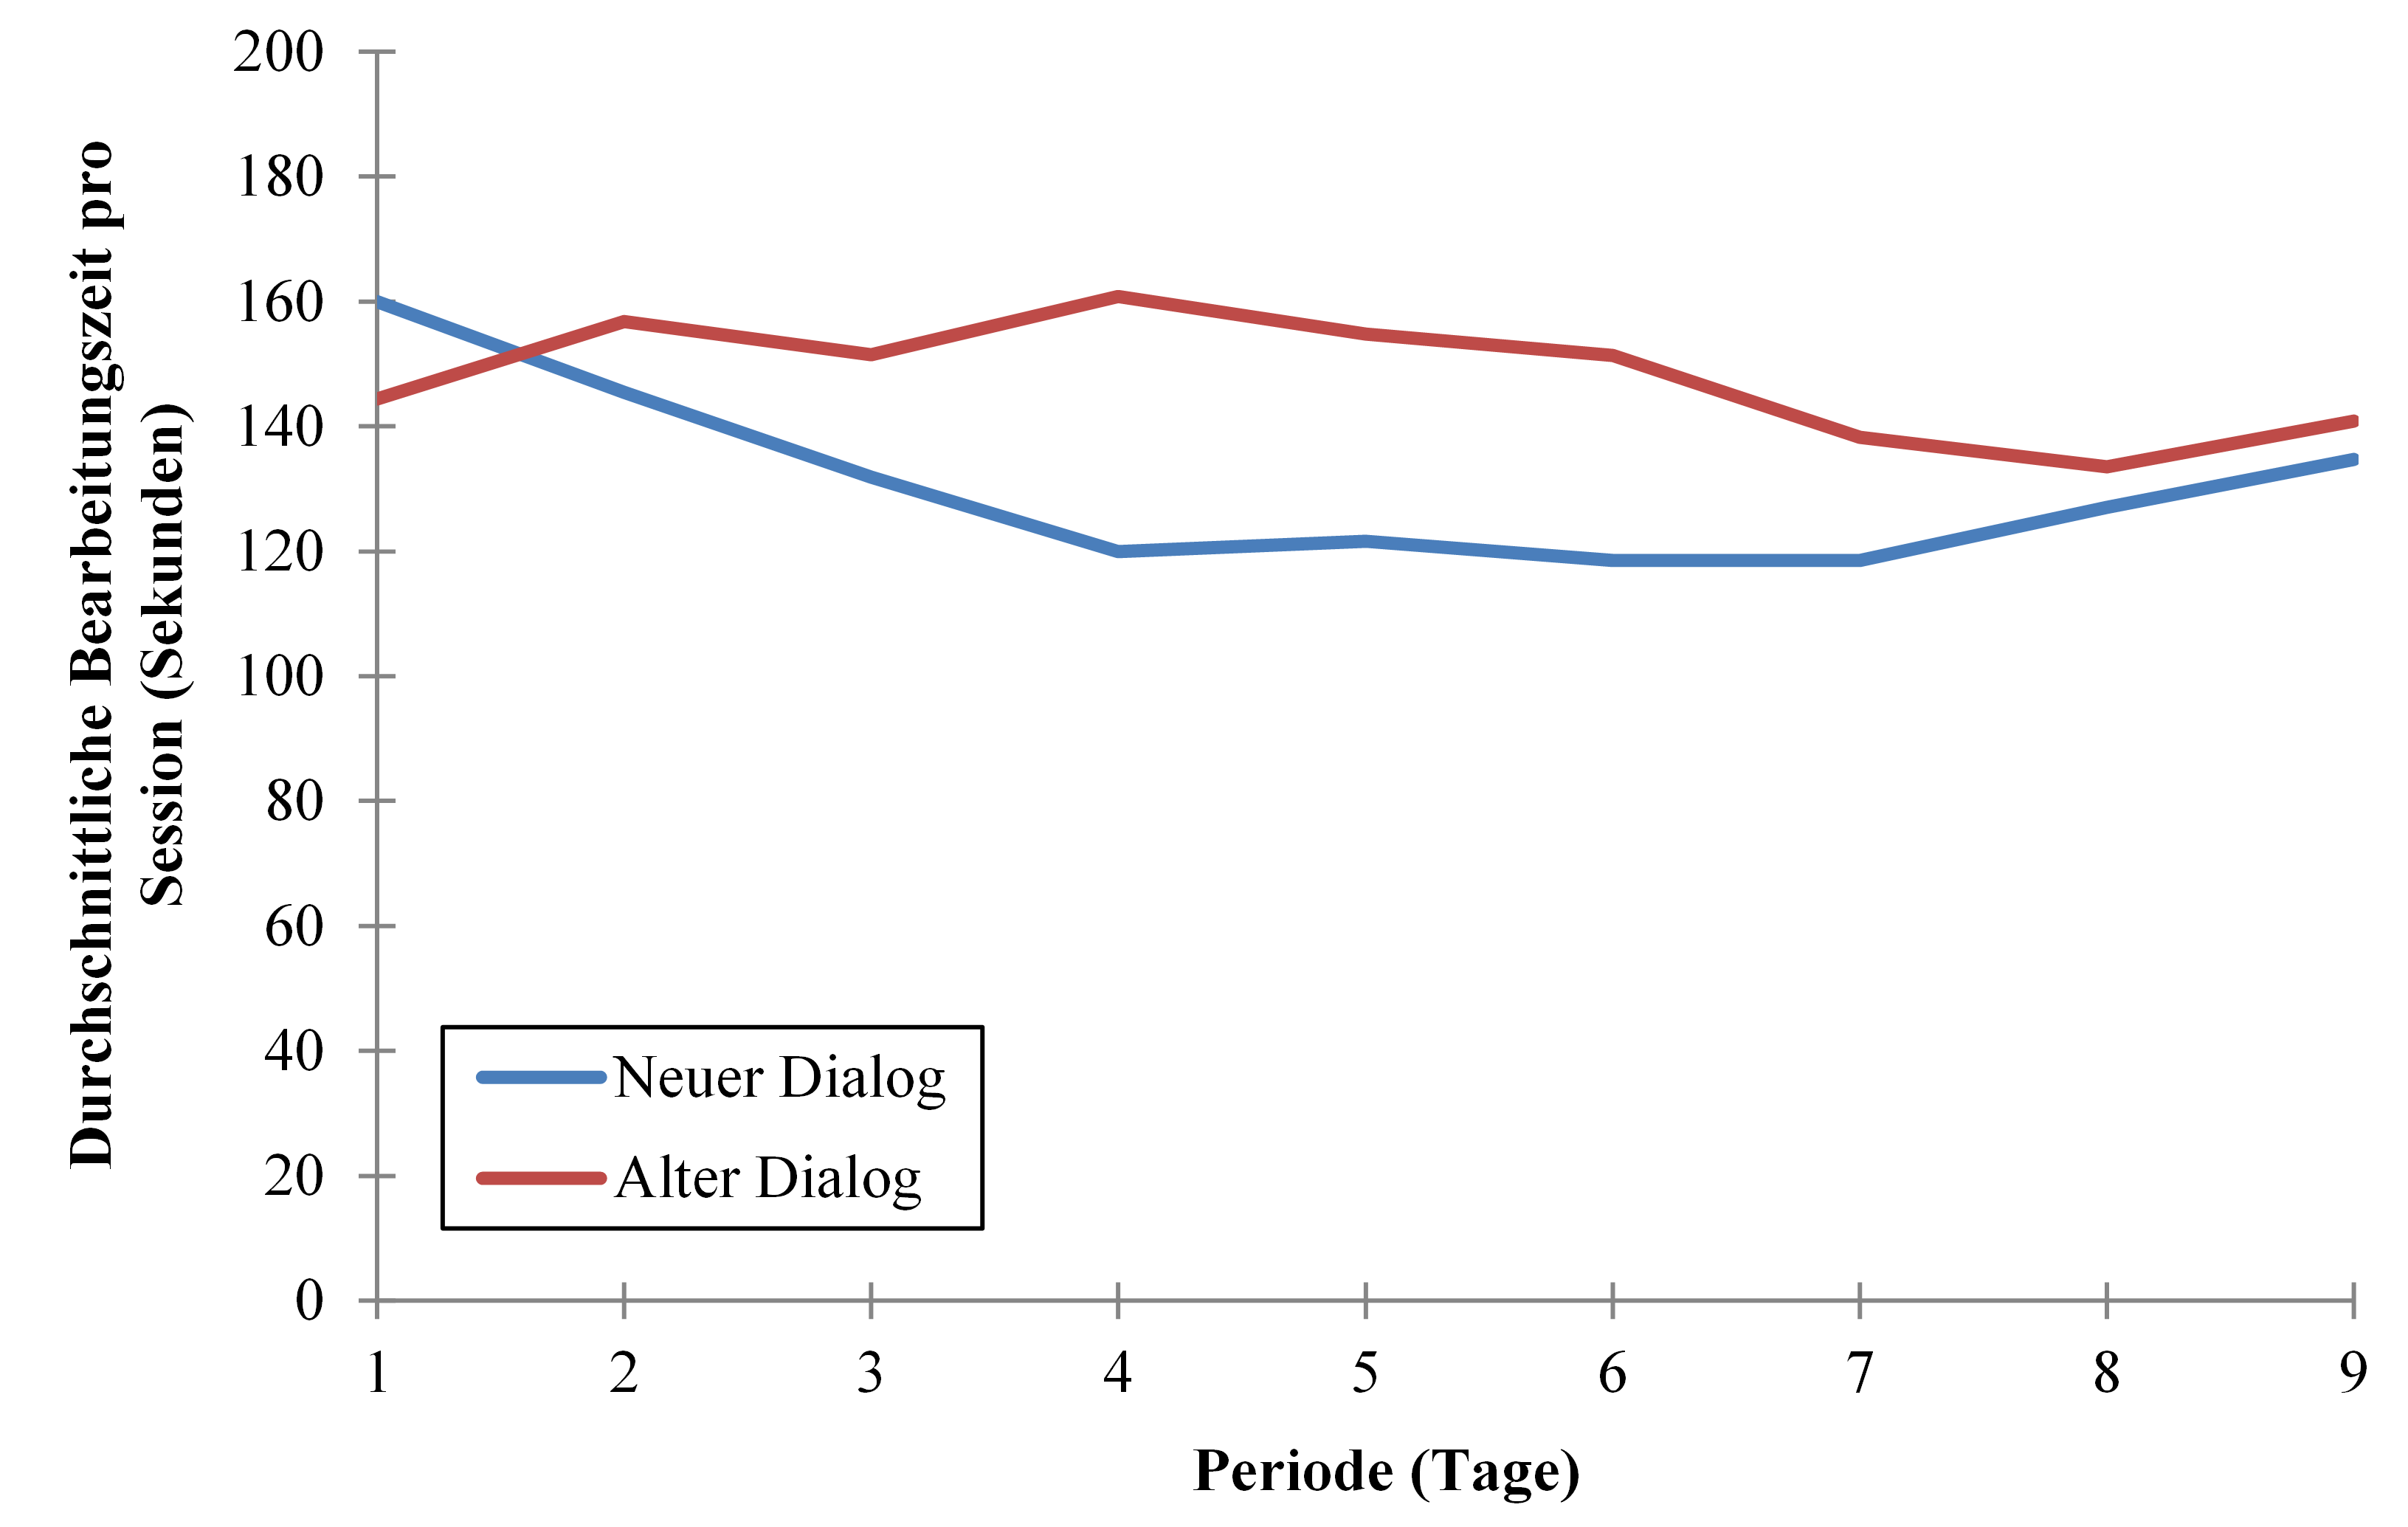
\includegraphics[]{img/Bearbeitungszeit_Verlauf.png}
  \caption{Vergleich des Verlaufs der durchschnittlichen Bearbeitungszeiten beider Dialoge.}
  \caption*{\textbf{Quelle:} Eigene Darstellung}
  \label{fig:BearbeitungszeitVerlauf}
\end{figure}
Es lässt sich erkennen, dass die durchschnittliche Bearbeitungszeit pro Session im alten Dialog (rote Linie) im Bereich von 140 Sekunden bis 160 Sekunden leicht schwankt. Zudem ist die gemittelte Bearbeitungszeit über alle Perioden mit 147 Sekunden, 14 Sekunden über der des neuen Dialogs (133 Sekunden).

Eine weitere Auffälligkeit innerhalb des Verlaufs des neuen Dialogs sind die ersten vier Perioden. In diesen sinkt die Bearbeitungszeit kontinuierlich von etwa 160 Sekunden auf durchschnittlich 120 Sekunden ab. Ab dort ist der Verlauf bis zum Ende der siebten Periode konstant. Anschließend steigt die Bearbeitungszeit wieder leicht auf 135 Sekunden an. Hingegen ist zu erkennen, dass die blaue Linie ab der zweiten Periode durchgehend unterhalb der roten Linie verläuft. Also die durchschnittliche Bearbeitungszeit im neuen Dialog, fast durchgängig geringer ist, als die im alten Dialog. Diese Tatsache sollte aber mit gewisser Vorsichtig betrachtet werden, da die Perioden, also sowohl der Wochentag als auch der anfallende Arbeitsaufwand an dem Tag, in denen die Erhebungen durchgeführt wurden nicht identisch sind.

\textbf{Mausklicks und Tastaturanschläge}

Als weitere Kennzahl für den Vergleich der Dialoge, dient die Anzahl von Interaktionen insgesamt, sowie deren Unterteilung in Mausklicks und Tastaturanschläge. Hiermit sollen Hinweise gesammelt werden, die dabei helfen können eine Aussage über die Komplexität und die physische Belastung bei der Arbeit mit den Dialogen zu treffen.

Als Erstes sollen die oben bereits ermittelten Bearbeitungsvorgänge genutzt werden, um alle Interaktionen zu bekommen. Es lässt sich anschließend mit Hilfe des Interaktions-Attributs \enquote{Typ} eine Unterscheidung zwischen Maus und Tastatur treffen. In Abbildung \ref{fig:verlaufInteraktionenAlterDialog} sowie in Abbildung \ref{fig:verlaufInteraktionenNeuerDialog} wurden die Interaktionen nach Typ gestaffelt gegen die Perioden in Tagen in einem Balkendiagramm aufgetragen. Die Datentabellen mit allen Werten zu den Interaktionen beider Dialoge ist im Anhang \ref{sec:datentabelleAlterDialog} bzw. \ref{sec:datentabelleNeuerDialog}zu finden. Es ist darauf zu achten, dass Interaktionen nur in ganzzahligen Werten in der Realität existieren. Die dargestellten Mittelwerte sind jedoch Dezimalzahlen mit zwei Nachkommastellen, um die Verhältnisse genauer darzustellen.
\begin{figure}[H]
  \centering
  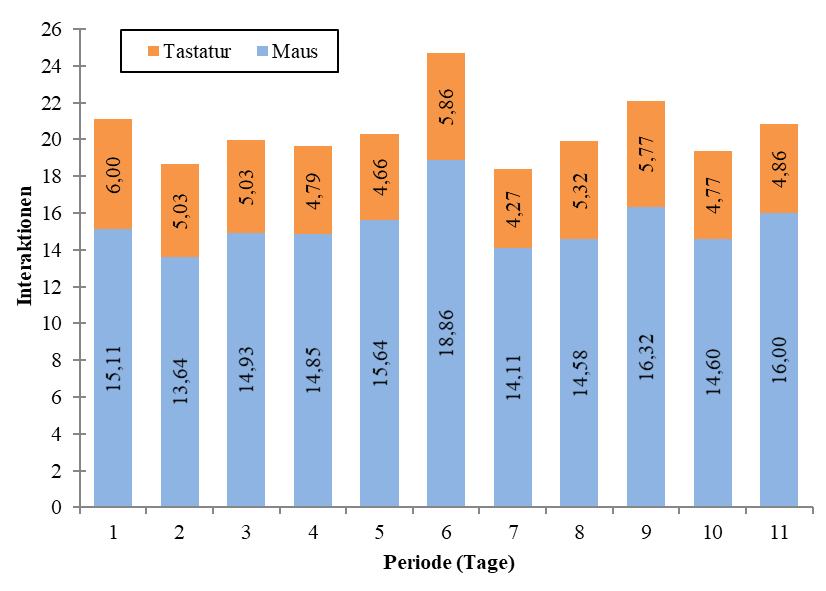
\includegraphics[]{img/Interaktionen_Alter_Dialog.png}
  \caption{Verlauf der Interaktionen im alten Dialog.}
  \caption*{\textbf{Quelle:} Eigene Darstellung}
  \label{fig:verlaufInteraktionenAlterDialog}
\end{figure}
Werden die Interaktionen pro Periode im alten Dialog betrachtet, lässt sich erkennen, dass die Werte pro Periode gerundet zwischen 18,4 und 24,7 Interaktionen schwanken. Werden Tastatur- und Maus-Interaktionen relativ zueinander erfasst, so wird die Tastatur zwischen 22,95\% und 28,42\% im Durchschnitt zu 25,06\% genutzt. Die Maus hingegen besitzt ein Maximum von 77,05\% und ein Minimum von 71,58\% an den gesamten Interaktionen einer Periode. Im Mittel wird die Maus zu 74,94\% verwendet.

\begin{figure}[H]
  \centering
  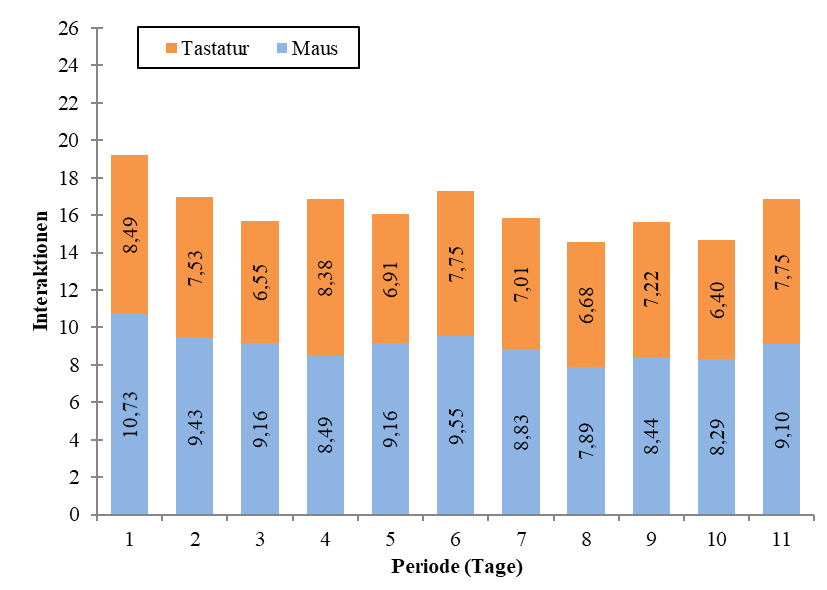
\includegraphics[]{img/Interaktionen_Neuer_Dialog.png}
  \caption{Verlauf der Interaktionen im neuen Dialog.}
  \caption*{\textbf{Quelle:} Eigene Darstellung}
  \label{fig:verlaufInteraktionenNeuerDialog}
\end{figure}
Im neuen Dialog ist zu erkennen, dass die Werte im Schnitt zwischen 14,5 und 19 Interaktionen liegen. Bei der Ermittlung von relativen Anteilen, liegt der Anteil von Tastatur-Interaktionen in einem Bereich von 41,67\% bis 49,67\%. Die anteilige Benutzung der Maus liegt zwischen 50,33\% und 58,33\%. Im Durchschnitt wird die Tastatur für 44,86\% und die Maus für 55,14\% der Interaktionen genutzt.

% Vergleich
Werden beide Dialoge miteinander verglichen so ist zum einen festzustellen, dass die Interaktionen im neuen Dialog geringere Schwankungen verzeichnen und zum anderen ist die durchschnittliche Anzahl von Interaktionen pro Session gemittelt über alle Perioden im alten Dialog etwa 25\% höher als im neuen Dialog. Zum anderen hat sich das Verhältnis von Tastatur- und Maus-Interaktionen verschoben. Mit dem neuen Dialog sind die Tastatur-Interaktionen um knapp 20\% gestiegen, dafür ist die Benutzung der Maus um 20\% zurückgegangen. Insgesamt wurden im neuen Dialog durchschnittlich pro Session knapp 4 Interaktionen weniger ausgeübt, als im alten Dialog.

\textbf{Anzahl und relative Häufigkeit von Veränderungen}

Wie bereits oben genannt wurden die Daten in zwei hintereinander liegenden Zeiträumen erhoben, in denen je nach aktuellem Aufkommen unterschiedlich viele Vorgänge mit unterschiedlichen Komplexitäten vorliegen. Die Komplexität soll im folgenden mit der Anzahl an Veränderungen bzw. den Eingaben von Daten auf der Oberfläche gleichgesetzt werden. Das heißt, umso mehr Daten einzugeben sind, desto komplexer ist die Bearbeitung des Vorgangs zu bewerten. Die Komplexität soll dabei helfen beide Stichprobenumfänge die Datengrundlage beider Dialog besser miteinander vergleichen zu können.

Um die Komplexität zu vergleichen wurde die relative Häufigkeit von Veränderungen gegen die Anzahl von Veränderungen (bis 50 Veränderungen) pro Session in einem Balkendiagramm (siehe Anhang \ref{sec:verteilungVeraenderungen}) aufgetragen. Aufgrund der Größe der Grafik wurde diese bewusst in den Anhang der Ausarbeitung verschoben. 

Der Komplexitätsvergleich wird auf der Grundlage von 777 Sessions aus dem neuen Dialog und 781 aus dem alten Dialog aufgestellt. Es fällt auf, dass die Verteilung von wenigen Veränderungen zu vielen Veränderungen innerhalb einer Session (gemessen am GD zweiter Ordnung) bei beiden Dialogen unterschiedlich aussieht. Der neue Dialog hat einen größeren Anteil von weniger komplexen Sessions (5 bis 13 Veränderungen). Im alten Dialog wiederum ist der Großteil der Sessions im Bereich von 11 bis 22 Veränderungen angesiedelt. Ab 35 Veränderungen ähneln sich beide Graphen wieder relativ stark. 


\textbf{Weitere Auffälligkeiten und Zusammenhänge}
%%%%%%%%%%%%%%%%%%%%%%%%%%%%%%%%%%%%%%%%%%%%%%%%%%%%%%%%%%%%%%%%%%%%%%%%%%%%

\subsection{Auswertung der Fragebögen}
\label{sec:auswertungDerFrageboegen}
Für die Auswertung der Fragebögen, die im Kapitel \ref{sec:durchfuehrungEvaluation} von den Probanden erhoben wurden, werden alle Datensätze in eine Excel-Tabelle übertragen. Daraufhin werden die Daten so angeordnet, dass jede Zeile einem Bewertungsaspekt aus dem ISO Fragebogen entspricht (siehe Abb. \ref{fig:auswertungsmatrixNeuerDialog} und Anhang \ref{sec:auswertungsmatrixAlterDialog}). Die Ausprägungen für die Bewertung eines Items werden so formatiert, dass sie anstatt von \enquote{$---$} bis \enquote{$+++$} den Werten von -3 (sehr negativ) bis +3 (sehr positiv) entsprechen. Dies hat den Vorteil das anschließend mit den numerischen Werten weiter gerechnet werden kann, da sie ein repräsentatives Abbild der Antworten darstellen und der Ordnung der Likert-Skala entsprechen\footnote{\cite[vgl.][]{Statista}}. Zudem wurden die Kennzahlen in den Auswertungsmatrizen farblich hinterlegt, damit zwischen negativen (rot) und positiven (grün) Bewertungen unterschieden werden kann. Das Rating der 35 Bewertungsaspekte wurde mit Hilfe der Mittelwerte aus den Bewertungen aller Teilnehmer berechnet. Die Benutzerzufriedenheit eines Gestaltungsgrundsatz wird ebenfalls durch den Mittelwert der fünf zuvor berechneten Mittelwerte der Bewertungsaspekte gebildet und besitzt anschließend einen Wert zwischen -3 und +3. Aus Darstellungsgründen wurden die Zahlen im Folgenden alle auf drei Stellen nach dem Komma gerundet.

In Abbildung \ref{fig:auswertungsmatrixNeuerDialog} sind alle Einschätzungen zu dem neuen Vermögensverzeichnis Dialog in aggregierter Form dargestellt. Stellt man diese Auswertungsmatrix in einen direkten Vergleich zu den Auswertungen des alten Dialogs (siehe Anhang \ref{sec:auswertungsmatrixAlterDialog}) lässt sich erkennen, dass der neue Dialog in allen sieben Gestaltungsgrundsätzen besser bewertet wurde, als der alte Dialog (siehe Abb. \ref{fig:vergleichBalkendiagramm}). 
\begin{figure}[H]
  \centering
  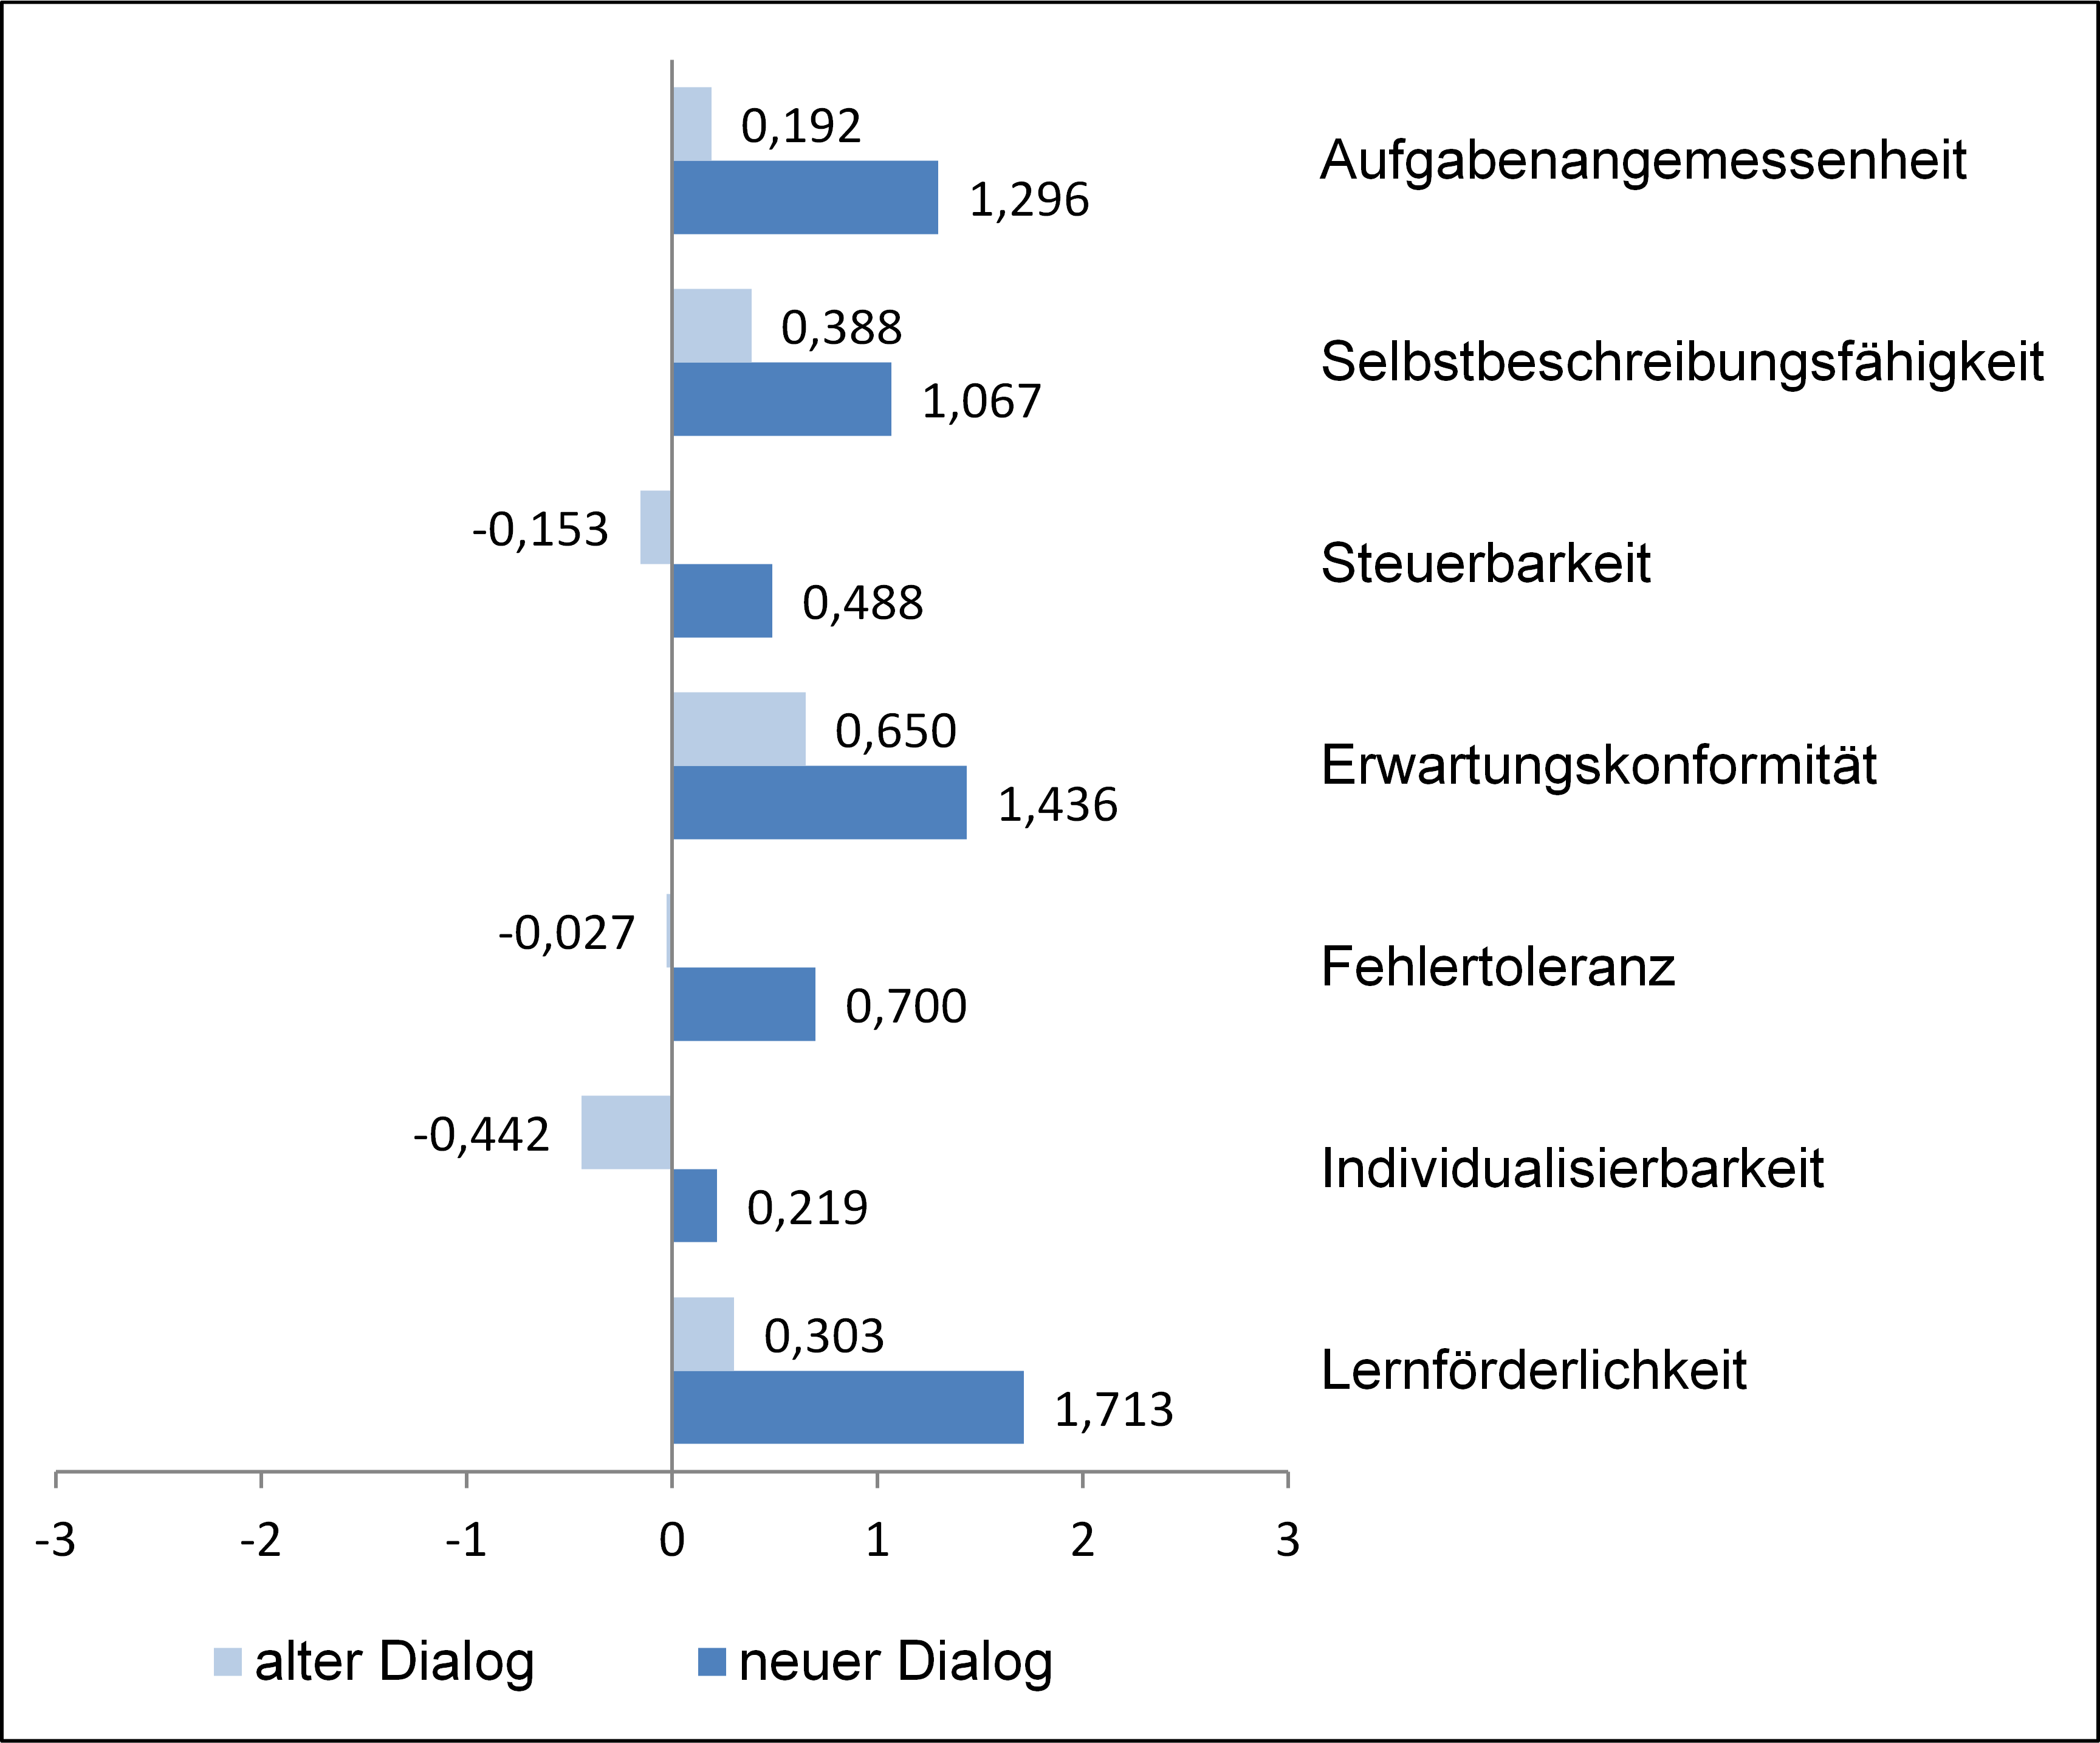
\includegraphics[]{img/ISO9241-10_Vergleich_Balkendiagramm.PNG}
  \caption{Vergleich der Gestaltungsgrundsätze zwischen altem und neuen Dialog.}
  \caption*{\textbf{Quelle:} Eigene Darstellung}
  \label{fig:vergleichBalkendiagramm}
\end{figure}
Die größte Steigerung kann in den Gebieten Aufgabenangemessenheit und Lernförderlichkeit mit 1,1 Punkten und 1,4 Punkten verzeichnet werden. Am wenigsten konnte die Benutzerzufriedenheit bei der Steuerbarkeit und der Individualisierbarkeit steigen. 

Trotz der insgesamt positiven Ergebnisse, gibt es immer noch Bereiche in denen die Bewertungen eher schwach ausfallen. Dazu zählt auch die Steuerbarkeit des Dialogs. Diese ist zwar positiv, also bietet ausreichend Freiheit bei der Bedienung, jedoch empfinden die Benutzer die Unterbrechungsfreiheit und die Anpassbarkeit von Informationsdarstellungen noch nicht vollkommen zufriedenstellend. Dieses Thema ist eher komplex zu bewerten, da hier auf die einzelnen Wünsche und Belangen der einzelnen Sachbearbeiter eingegangen werden müsste, um weitere Verbesserungen zu erzielen.

Auch die Kategorie Individualisierbarkeit selbst konnte im direkten Vergleich einen Gewinn von knapp 0,7 Punkte verzeichnen. Jedoch liegt die Bewertung mit +0,219 im unteren positiven Bereich. Besonders die Punkte \enquote{Erweiterbarkeit durch den Benutzer} und \enquote{Individuelle Anpassbarkeit durch den Benutzer} fallen beide noch schlecht aus. Gleichzeitig sind die beiden Bewertungsaspekte, trotz ihres Anstiegs um 0,4 bzw. 0,6 Punkten, auch die einzigen die noch negativ bewertet wurden. Sie spiegeln die individuelle Erweiterbarkeit und Anpassbarkeit von Bearbeitungsschritte und Benutzer wider. Die Kritik an dieser Stelle ist aber durchaus nachzuvollziehen, da sich der Dialog nur an wenigen Stellen individuell anpassen lässt. Ein Grund dafür ist die niedrige Priorisierung von individuellen und dynamischen Strukturen während der Konzeptionsphase. Es ist denkbar in einem nachfolgenden Projekt noch einmal explizit auf die beiden Aspekte und Benutzeranliegen einzugehen, um bestenfalls die Benutzerzufriedenheit weiter zu verbessern.

Insgesamt ist die Selbstbeschreibungsfähigkeit mit einem Wert von +1,067 durchaus zufriedenstellend. In Bezug auf die, durch den Benutzer geforderten und die durch das System automatisierten Erklärungen, ist aber noch klar ein Verbesserungspotential zu erkennen. Hier könnten gezielte Maßnahmen eingeleitet werden, bei denen zusammen mit dem Fachbereich fehlende Erklärungen evaluiert und anschließend ergänzt werden. Dies sollte einen vergleichsweise geringen Aufwand darstellen und kann auf der anderen Seite große Effekte erzielen.

Mit dem Blick auf die positiven Eigenschaften des neuen Vermögensverzeichnis Dialogs fallen unter die besten fünf Punkte:
\begin{enumerate}
    \item Hilfe beim Behalten von Gelerntem (+2,104),
    \item Autodidaktisch\footnote{Autodidaktisch = Wissen durch Literatur, Übungen, Beobachtungen oder Versuche eigenständig aneignen } (+2,085),
    \item Bedienungskomplexität (+2,083),
    \item Zeit für Einarbeitung (+2,063) und
    \item Erfordernis, sich Details zu merken (+1,979).
\end{enumerate}
Interessant ist, dass vier der fünf Punkte aus dem Bereich Lernförderlichkeit stammen. Der Aspekt \enquote{Bedienungskomplexität} wiederum gehört zum Grundsatz Aufgabenangemessenheit. Hier bewerten die Benutzer die Bedienung des neuen Dialogs, mit einem durchschnittlichen Schwellwert von etwa +2, als angenehm und einfach. Im Vergleich ist dies ein Anstieg von über 1,6 Punkten. Die gestiegene Benutzerzufriedenheit von über 1,4 Punkten im Bereich der Lernförderlichkeit kann genauso wie die Bedienungskomplexität durch die Vereinfachung und Verringerung von Informationen, Bedienelementen und Strukturen erklärt werden. 
\begin{figure}[H]
  \centering
  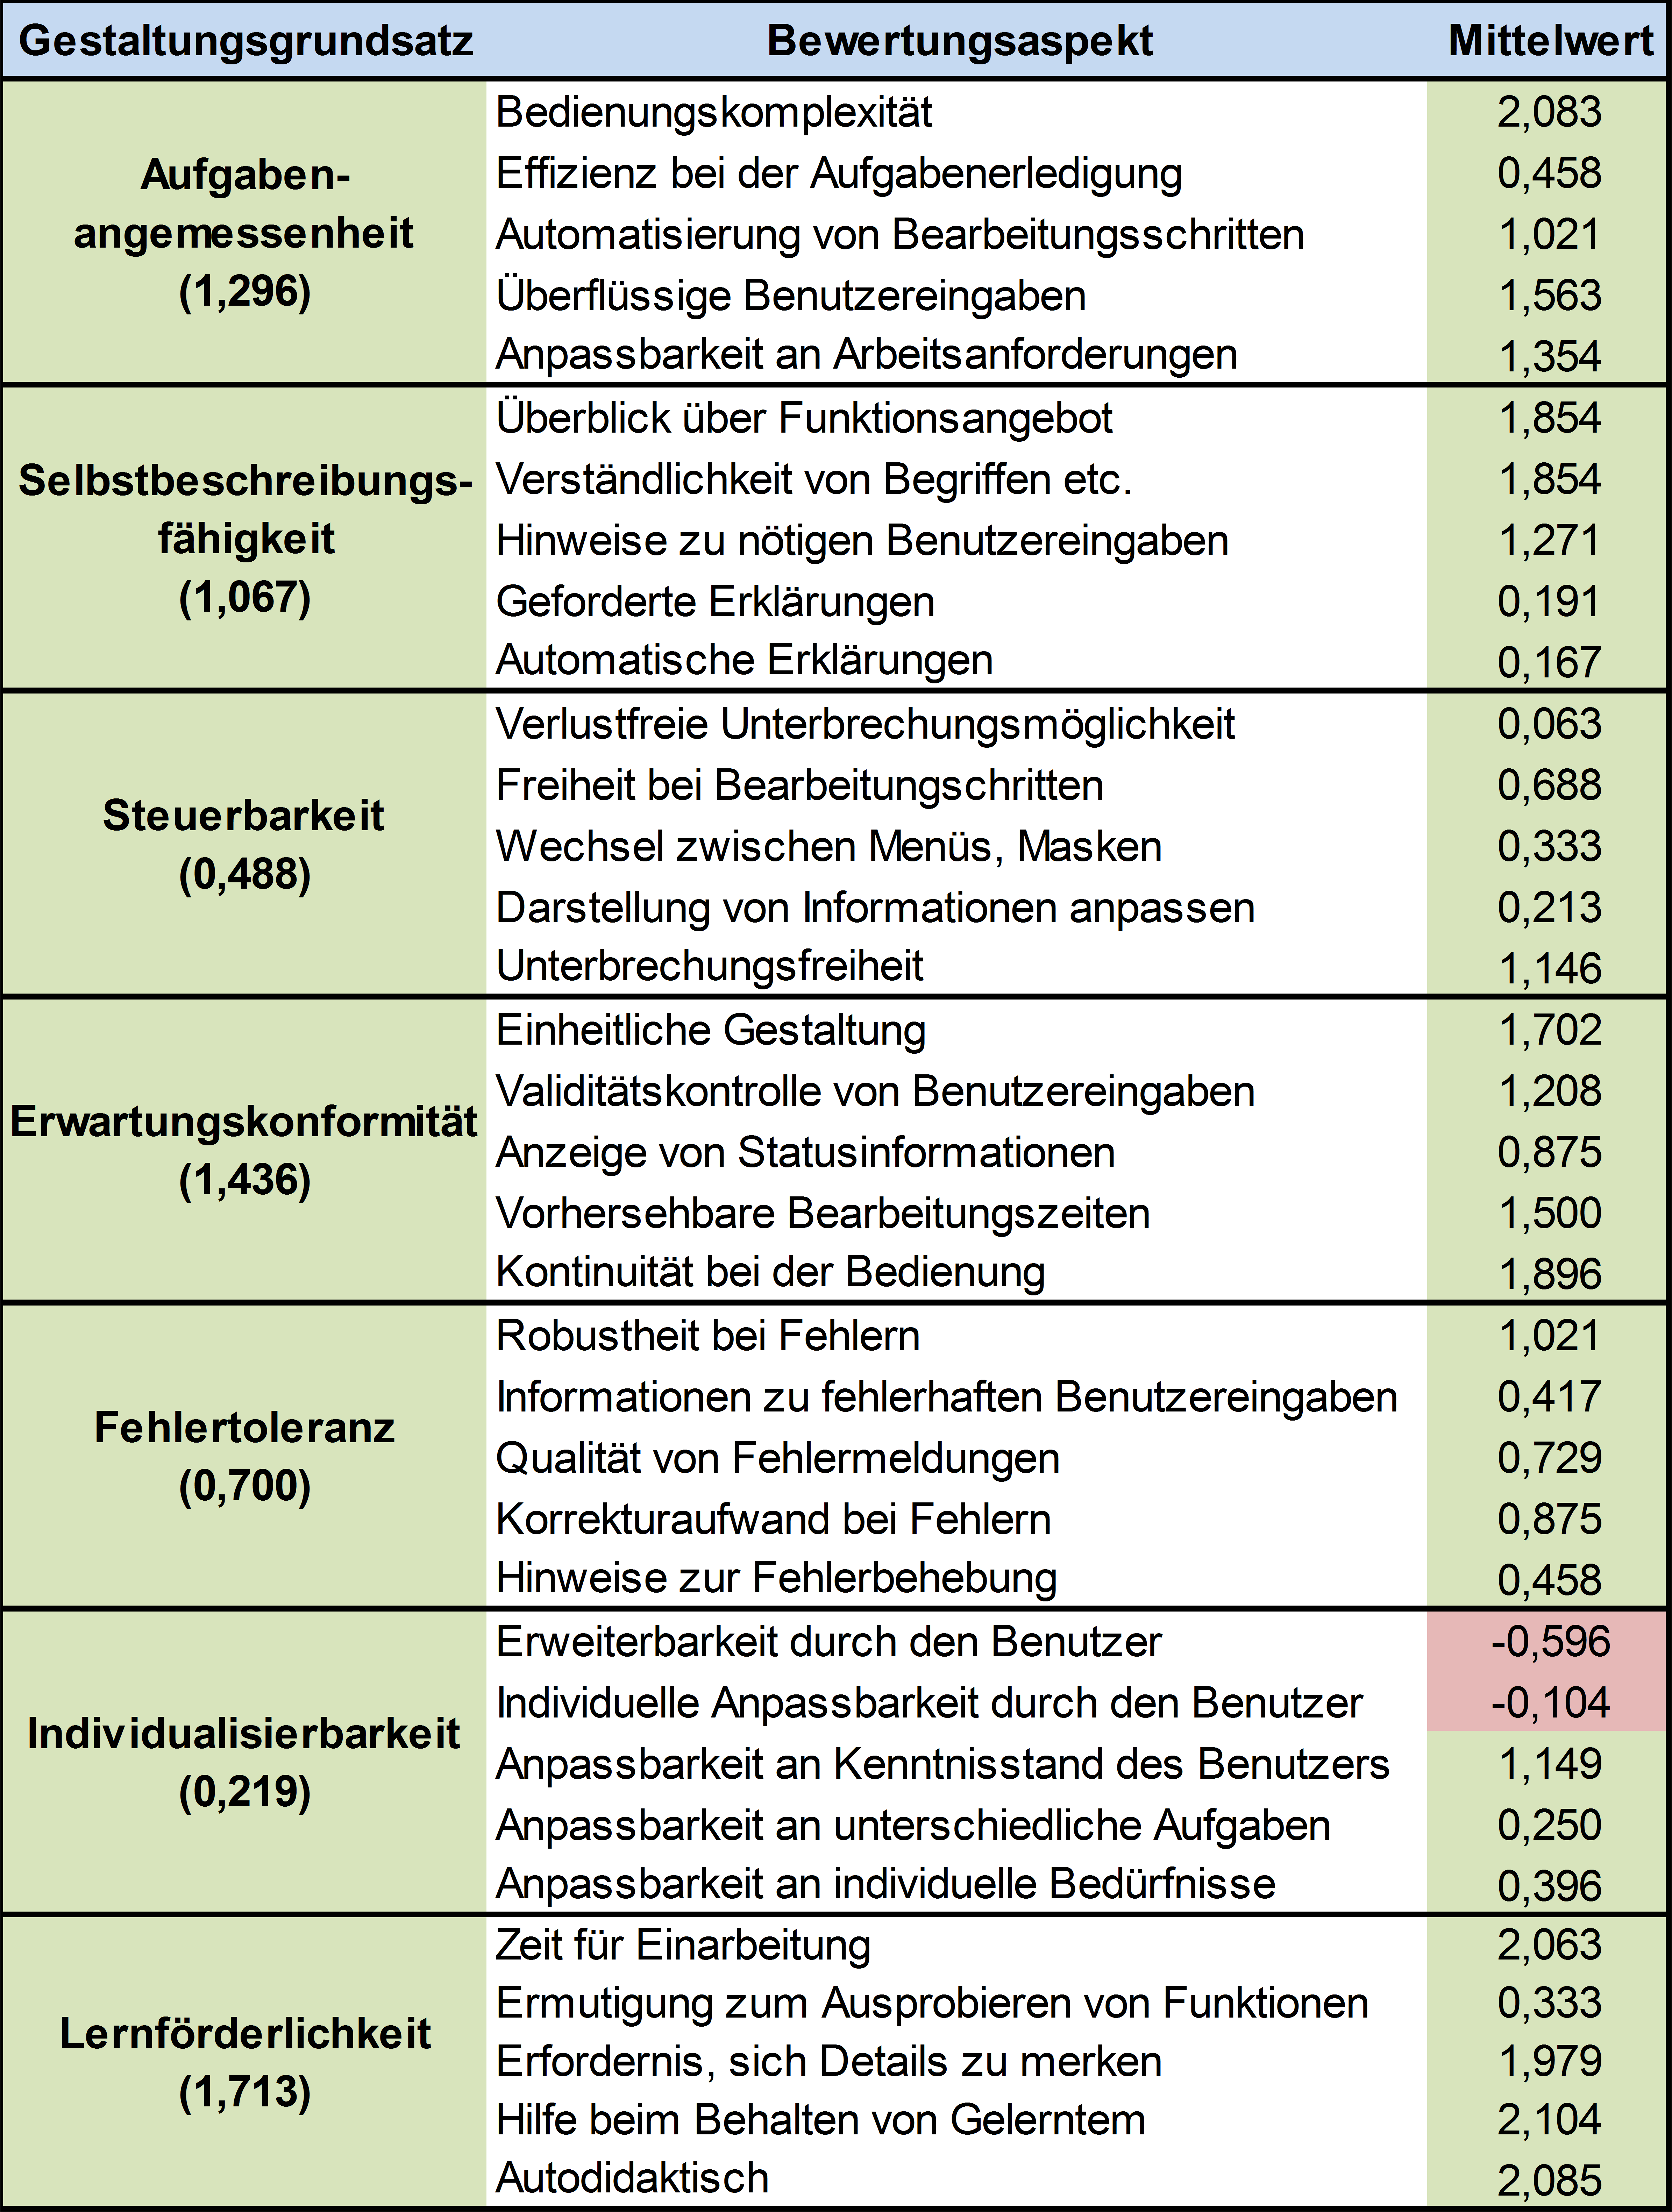
\includegraphics[width=430px]{img/Auswertungsmatrix_Neuer_Dialog.PNG}
  \caption{Auswertungsmatrix zum ISO 9241-10 Fragebogen neuer Dialog.}
  \caption*{\textbf{Quelle:} Eigene Darstellung}
  \label{fig:auswertungsmatrixNeuerDialog}
\end{figure}
Die fünf Bewertungsaspekte sollten gerade mit Blick auf die Zeit positive Auswirkungen haben. Fällt die Betrachtung auf die Punkte zwei und vier so lässt sich ableiten, dass potentiell künftig Zeit eingespart werden kann. Es muss sich lediglich der Anwendungsfall \enquote{Neuer Mitarbeiter} vorgestellt werden. Der neue Mitarbeiter benötigt tendenziell weniger Zeit für die Einarbeitung in den neuen Dialog. Zudem kann der zeitliche Aufwand für helfende und einweisende Kollegen verringert werden.

So lassen sich auch die Punkte \enquote{Erfordernis, sich Details zu merken} und \enquote{Hilfe beim Behalten von Gelerntem} mit einer gesteigerten Effizienz in Verbindung bringen. Ein möglicher Anwendungsfall hierfür ist ein Vermögensverzeichnis, das viele Details enthält. Hier muss der Sachbearbeiter im Gegensatz zum alten Dialog nur noch einen Bruchteil der Informationen übernehmen und somit auch weniger Informationen gleichzeitig im Gedächtnis behalten. Dies kann durchaus positive Effekte auf die Bearbeitungszeit und die mentale Belastung des Sachbearbeiters nehmen.

Im Gesamtüberblick kann bereits ein erfreulicher Verlauf der Benutzerzufriedenheit in allen sieben Grundsätzen verzeichnet werden. Hieraus lässt sich bereits auf eine gewisse Effektivität des Projekts schließen, besonders mit Bezug auf die zeitlichen Effekte. Die Benutzer scheinen allgemein zufriedener bei der Arbeit mit dem neuen Dialog.

%%%%%%%%%%%%%%%%%%%%%%%%%%%%%%%%%%%%%%%%%%%%%%%%%%%%%%%%%%%%%%%%%%%%%%%%%%%%

\subsection{Abschließende Ergebnisdiskussion}
\label{sec:abschliessendeErgebnisdiskussion}
Im letzten Schritt werden die gesammelten Erkenntnisse zusammengefasst und in einen Zusammenhang gebracht. Zusätzlich werden die Ergebnisse mit weiteren Argumenten und verschiedenen Blickrichtungen angereichert, um abschließend die drei Hypothesen H1\textsubscript{0}, H2\textsubscript{0} und H3\textsubscript{0} zu belegen bzw. zu widerlegen. Das Ziel ist es ein abschließendes Ergebnis für die Evaluation bzw. die Zielerreichung der Abschlussarbeit zu erhalten.

% Hypothese H1
Hinsichtlich der ersten Hypothese H1\textsubscript{0} ist mit den vorliegenden Fakten und Annahmen zu überprüfen, ob diese belegt werden kann oder nicht. Werden Argumente gesucht und vorliegende Erkenntnisse verwendet, um die Nullhypothese zu widerlegen, so könnte argumentiert werden, dass aufgrund der Verteilung von Veränderungen, die bereits in der Logfile-Auswertung dargelegt wurde, eine höhere Komplexität im Testzeitraum des alten Dialogs vorlag. Somit ist davon auszugehen, dass eine höhere Komplexität auch zu einer erhöhten Bearbeitungszeit geführt haben könnte. Auf der anderen Seite kann diese Contra Argument auch in gewisse Weise relativiert werden, da die gemessene Komplexität nur die Anzahl von Veränderungen misst und nicht spezifisch die Art der Veränderungen mit einbezieht. Das heißt eine Vielzahl von Veränderungen, die lediglich das Anklicken von Checkboxen beinhalten, sind nicht unbedingt komplexer als wenige Änderungen, die das Ausfüllen von Textfeldern benötigen, einzuschätzen. Über die genaue Komplexität lässt sich mit den vorliegenden Auswertungen keine eindeutige Auskunft geben. Ein weiterer Fakt, der gegen die Nullhypothese spricht ist, dass in beiden Erhebungszeiträumen nicht die selben Sachbearbeiter teilgenommen haben. Aufgrund von Urlaub, Krankheit oder keinen Arbeitsaufträgen kann es möglich gewesen sein, dass Mitarbeiter die sehr effizient Arbeiten, überwiegend im Testzeitraum des neuen Dialogs anwesend waren und somit die Bearbeitungszeit positiv beeinflusst haben. Jedoch könnte auch genau der umgekehrte Sachverhalt vorgelegen haben, wodurch der Positive Effekt dem alten Dialog zugesprochen werden müsste.

Mit Blick auf Erkenntnisse die für die Nullhypothese sprechen ist klar die verbesserte durchschnittliche Bearbeitungszeit von etwa 14 Sekunden anzubringen. Ebenfalls lässt die anfänglich sinkende Kurve (siehe Abb. \ref{fig:BearbeitungszeitVerlauf}) auf einen Lerneffekt schließen, der möglicherweise auch noch nicht abgeschlossen ist und bei vermehrter Benutzung noch weiter wächst. Einhergeht die Tatsache das eine verringerte Anzahl von Interaktionen gemessen wurden die darauf schließen können das auch weniger Zeit benötigt wird. Damit zusammenhängend lässt sich argumentieren, da sich das Verhältnis von Maus- und Tastatur-Interaktionen zugunsten der Tastatur entwickelt hat und die Sachbearbeitung schneller mit der Tastatur arbeiten, dass dadurch die Zeit gesunken ist. Unterbewusste Effekte könnten zudem durch die übersichtlichere Oberfläche und der damit vereinfachten Eingabe von Informationen einhergegangen sein. Dies bestätigt auch die Auswertung der Fragebögen, bei der festgestellt werden konnte, dass die Sachbearbeiter den neuen Dialog einfacher empfinden und sich mit diesem weniger Informationen merken müssen. Daraus ist zu schließen, dass Sachbearbeiter weniger Fehler machen und seltener Informationen erneut im Vermögensverzeichnis nachschauen müssen und daher schneller den Vorgang bearbeiten konnten. Ein vermutlich nicht ganz unerhebliches Argument, das ebenfalls für die Nullhypothese sprechen kann ist, dass die Sachbearbeiter während des Testzeitraums des neuen Dialogs mehr auf das Entdecken von Funktionen und die Einarbeitung mit dem Dialog fokussiert waren. Dabei haben sie dann weniger auf den alltäglichen Zeitdruck reagiert und eventuell nicht unter Voll-Last und maximaler Geschwindigkeit die Vorgänge bearbeitet.

Werden die Pro und Contra Argumente zusammengefasst, so lässt sich für die Hypothese H1\textsubscript{0} eine Überzahl an Fakten, die für eine Verbesserung der durchschnittlichen Bearbeitungszeit pro Bearbeitungsvorgang sprechen, erkennen. Demnach kann H1\textsubscript{0} fast uneingeschränkt bestätigt werden und wird daher als belegt anerkannt und die H1\textsubscript{A} kann verworfen werden.

% Hypothese H2
Als nächstes ist die Hypothese H2\textsubscript{0} hinsichtlich ihrer Wahrheit zu prüfen. Ein Contra-Argument das gleich zu dem der Hypothese H1\textsubscript{0} entgegengebracht werden kann ist die Verteilung der Veränderungen. Auch hier sollte aber wie bereits erwähnt eine eher kritische Haltung eingenommen werden, da Informationen zur Art der Veränderungen nicht vorliegen und es somit keine eindeutige Komplexitätssteigerung gegeben haben muss. 

Eindeutig für die Nullhypothese und gegen die Antithese H2\textsubscript{A} ist die Auswertungsstatistik unter dem Punkt \enquote{Mausklick und Tastaturanschläge} einzubringen. Diese zeigt eine klar gesunkene Tendenz, mit durchschnittlich etwa 4 Interaktionen pro Bearbeitungsvorgang weniger. Die eher als gering einzuschätzenden Schwankungen (siehe Abb. \ref{fig:verlaufInteraktionenNeuerDialog}) deuten ebenfalls auf eine Kontinuität hin und weniger auf eine glückliche Datenlage. Weitergehend ist die logische Schlussfolgerung aus einer verringerten Menge an Bedienelementen auf der Oberfläche das weniger Schritte (Interaktionen) benötigt werden um von einem Punkt zu einem anderen zu navigieren. Dies unterstützen auch nochmal die positiven Rückmeldungen aus dem Fragebogen, die für eine gestiegene Übersichtlichkeit und eine gesunkene Bedienkomplexität sprechen.

Bei dem Zusammenschluss aller Argumente ist auch bei der Hypothese H2\textsubscript{0} zu sehen, dass mehr bestätigende als verwerfende Fakten genannt werden können. Auch hier ist mit einer gewissen Unsicherheit für die Nullhypothese H2\textsubscript{0} und somit für eine durchschnittlich gesunkene Anzahl von Interaktionen pro Bearbeitungsvorgang zu tendieren. Damit einhergehend wird die Antithese H2\textsubscript{A} verworfen.

%Hypothese H3
Die letzte Hypothese H3\textsubscript{0}, die es zu überprüfen gilt, hat keine offensichtlich widerlegenden Fakten anzuführen. Hingegen sprechen mehrere Sachverhalte für die Nullhypothese. Eines dieser Sachverhalte ist die Auswertung des Fragebogens. Hier konnten in allen sieben Grundsätzen der Norm 9241-110 nur Verbesserungen verzeichnet werden. Auch wenn es in manchen Bereichen noch Potential für Steigerungen gibt, ist die grundsätzliche Haltung zum neuen Dialog positiv anzusehen. Die bereits belegten Hypothesen H1\textsubscript{0} und H2\textsubscript{0} sind ebenfalls ein Argument für die gestiegene Software-Ergonomie. Ein Fakt der schon während der Entwicklungsphase der neuen Oberfläche aufgekommen ist, ist das positive Feedback aus den Prototypen-Tests der Sachbearbeiter.

Die vorliegende Argumentationsstruktur kann ziemlich eindeutig als Bestätigung des Nullhypothese H3\textsubscript{0} genutzt werden. Damit lässt sich feststellen, dass die Benutzer den neuen Dialog als ergonomischer empfinden als den alten Dialog. In dem Zuge kann H3\textsubscript{A} verworfen werden.

% Forschungsfrage beantworten
Nachdem alle drei Hypothesen als bewiesen belegt wurden, soll abschließend auf die Forschungsfrage der Abschlussarbeit eingegangen werden. Für die Beantwortung der Forschungsfrage werden die Hypothesen, die im Rahmen dieser Abschlussarbeit überprüft wurden, genutzt. Um auf die Frage umfassend eingehen zu können wird diese in drei Teile zerlegt. 

Der Begriff Gebrauchstauglichkeit setzt sich aus drei Kriterien zusammen. Der Effektivität, der Effizienz und der Zufriedenheit von Anwendern. Die Effektivität beschreibt das Ausmaß und die Erreichung von Zielen. In diesem Fall ist das Ziel der Benutzeroberfläche die Eingabe von Vermögensverzeichnissen zu ermöglichen. Da die neue Oberfläche in dazu in der Lage war die Bearbeitungsvorgänge während des Testzeitraums abzubilden und den Sachbearbeitern ausreichend Funktionalitäten zur Bearbeitung zur Verfügung zustellen ist die Effektivität im gleichen Maße wie die der alten Oberfläche einzuschätzen.

Die Effizienz ist ein weiterer Parameter der über die Ausprägung der Gebrauchstauglichkeit einer Software entscheidet. Die Effizienz definiert sich über den Aufwand der zur Erreichung des Ziels benötigt wird. Auf den Kontext bezogen lässt sich die Effizienz sowohl aus dem physischen, dem psychischen Aufwand und der benötigten Zeit zusammensetzen. Sowohl die physische als auch die psychische Belastung zeigt eine positive Tendenz, die sich mit Hilfe der Hypothesen H2\textsubscript{0} und den Erkenntnissen aus der Umfrage für den neuen Dialog erklären lässt. Durch eine geringere Anzahl von Interaktionen können gleichzeitig wiederholende Bewegung von Schultern, Armen, Händen und Fingern verringert werden. Darüber hinaus werden durch eine geringere Anstrengung des Gedächtnisses und der Wahrnehmungsfähigkeit, die daraus resultieren das die Oberfläche übersichtlicher geworden ist und nur noch die nötigen Informationen beinhaltet, die kognitiven Fähigkeiten weniger beansprucht. Der dritte Bestandteil der Gebrauchstauglichkeit ist die Zufriedenheit. Diese greift die subjektive Wahrnehmung der Anwender und das Erlebnis bei der Benutzung von Benutzerschnittstellen auf. Die Zufriedenheit kann aufgrund der positiven Umfrageergebnissen bzw. der belegten Hypothese H3\textsubscript{0}, ebenfalls als verbessert angesehen werden.

Zusammengefasst ist davon auszugehen, dass zumindestens die Effizienz und Zufriedenheit und somit die Gebrauchstauglichkeit der neuen Benutzeroberfläche höher einzuordnen ist, als die der alten Benutzeroberfläche. Das Ziel der Abschlussarbeit konnte also, durch das Zusammenspiel von theoretischen Grundlagen und fundiertem Wissen zur Gestaltung ergonomischer Benutzerschnittstellen, einem agilen und Anwender nahen Prozessvorgehen bei der Erarbeitung der neuen Benutzerschnittstelle und einer hinreichenden Auswahl an Evaluationsmethoden, im vollen Umfang erreicht werden.

\section{Resümee und Ausblick}
Als Abschluss des Projekts soll über den Verlauf und die Ergebnisse reflektiert werden. Darüber hinaus wird ein Ausblick zu möglichen Maßnahmen, die im Anschluss an das Projekt durchgeführt werden können, gegeben.

% Verlauf - Vorgehen in der Praxis rentabel?
Insgesamt kann das Projekt als erfolgreich abgeschlossen bezeichnet werden. Das primäre Projektziel wurde vollständig erreicht. Zudem hat das Projekt mit dem UIDataCollector ein Nebenprodukt abgeworfen, das es ermöglicht zukünftig strukturierte Aufzeichnungen von Interaktionen durchzuführen.

Mit Blick auf den Projektaufwand, ist die Rentabilität jedoch kritisch zu betrachten. Grundsätzlich scheint ein agiles Vorgehen in der Software-Entwicklung, besonders im Bereich von Oberflächen, ein sinnvoller Ansatz zu sein. Der Entwickler bekommt im Gegensatz zu klassischen Modellen einen viel präziseren Blick für die Anforderungen und die Anwender, für die die Schnittstelle konzipiert wird. Auf der anderen Seite hat sich herausgestellt, dass ein derartiger Aufwand für die Evaluation als \enquote{Ein-Mann-Projekt} schwierig zu bewältigen. Daher ist es in der Praxis empfehlenswert entweder eine abgespeckte Form der Evaluation durchzuführen oder in einem kleinen Team, das sich die Aufgaben untereinander aufteilen kann, zu arbeiten. 

Bei der Evaluation einer Schnittstelle ist sowohl die Methode schriftliche Befragung via Fragebogen als auch die Logfile-Erhebung zu empfehlen. Mit den Ergebnissen der Isonorm Fragebögen, können viele Informationen über die Meinung und Zufriedenheit der Anwender gewonnen werden. Durch das eigens entwickelte Tool, zur Aufzeichnung von Interaktionen, konnten sehr generische Daten erhoben werden. Aus diesen ließen sich eine Vielzahl von Erkenntnissen gewinnen, die für die Bewertung der Oberflächen genutzt werden konnten. Der Vorteil an der eigenen Entwicklung ist, dass von Projekt zu Projekt entschieden werden kann in welchem Detailgrad die Daten erhoben werden sollen. Umso generischer die Daten gesammelt werden, desto höher ist der Aufwand für die anschließende Aggregation und Auswertung einzuschätzen.

% gesparte Bearbeitungszeit pro Jahr
Rückblickend soll auch der Nutzen des Projekts etwas genauer verdeutlicht werden. Dazu wird, anhand der Ergebnisse in Kapitel \ref{sec:auswertungDerLogfiles}, die zeitliche Einsparung für die Bearbeitung eines Vorgangs auf ein Jahr hochgerechnet. Es wird von 68 Bearbeitungsvorgängen pro 80 Sachbearbeiter und pro Tag ausgegangen. Zudem wird von den ermittelten 14 Sekunden Einsparung pro Bearbeitungsvorgang ausgegangen. Wird nun auf 230 Arbeitstage im Jahr und insgesamt 550 Sachbearbeiter hochgerechnet und dies anschließend auf \enquote{Ganz-Tages-Kräfte} (GTK) umgerechnet, so erhält man aufgerundet 52 GTK's, die pro Jahr mit der neuen Benutzeroberfläche eingespart werden könnten. Die Kennzahl gibt keine vollständige Sicherheit. Jedoch sollte sie ein Indiz für die Wirkungsrichtung des Projekts aufzeigen können.

Als Fazit lässt sich schließen, dass es sich lohnen kann Benutzeroberflächen zu erneuern bzw. zu überarbeiten. Besonders Oberflächen, die mit der Zeit an Komplexität dazugewonnen haben und dadurch unübersichtlich und ineffizient wurden, sind Kandidaten für eine Neuauflage. Dabei kann es durchaus sinnvoll sein mit Hilfe von Evaluationsmethoden eine bestehende Benutzerschnittstelle auf Schwächen und Stärken zu analysieren, um gegeben falls eine neue Oberfläche zu entwerfen. Ebenfalls können die Methoden dazu eingesetzt werden, den Unterschied von Oberflächen bewerten zu können. Bei der Konzeption hat es sich ebenfalls als hilfreich erwiesen, ein agiles Vorgehen zu verfolgen. Dieses besitzt seine Stärken in der inkrementellen und  Nutzungskontext nahen Entwicklung 

% Ausblick
In der kurz- bis mittelfristigen Zukunft, ist es angedacht mit dem neu entwickelten Dialog weiterzuarbeiten, um bestenfalls den alten Dialog komplett ablösen zu können. Wie bereits angesprochen ist es auch denkbar, dass Logfile-Erhebungen weiterhin zum Einsatz kommen, um Oberflächen und deren Nutzungskontext genauer bewerten zu können. Mit Hilfe der gewonnen Erfahrungen und Erkenntnisse aus diesem Projekt, können zukünftig weitere Oberflächen überarbeitet werden. Langfristig sollte es das Ziel sein, dass alle Oberflächen die umliegenden Bearbeitungsprozesse des Inkassoverfahrens optimal unterstützen.
	
%%%%%%%%%%%%%%%%%%%%%%%%%%%%%%%%%%%%%%%%%%%%%%%%%%%%%%%%%%%%%%%%%%%%%%%

\section*{Danksagung}
\addcontentsline{toc}{section}{Danksagung}
\fancyhead[R]{Danksagung}
Ich möchte mich hiermit bei allen Personen bedanken, die mich im Kontext meiner Bachelorarbeit, sei es im Projektgeschehen oder der Ausarbeitung selbst, unterstützt haben. Besonders möchte ich mich bei meinem Mentor Prof. Dr. Carsten Weigand, für seine freundliche, schnelle und unkomplizierte Kommunikation und Betreuung bedanken. Ebenso gebührt meinen Arbeitskollegen ein Dankeschön, für sämtliche konstruktive Kritik und Meinung, sowie der Unterstützung während des Projekts. Ich möchte mich auch bei meiner Familie, Freunden und speziell meiner Freundin bedanken, die mir jeder Zeit als Hilfe zur Verfügung stand und mir immer wieder bei Problemen weiter geholfen hat. Ich bin mit dem Projektverlauf und dem Endergebnis sehr zufrieden und möchte den Projektbeteiligten für die rege Zusammenarbeit meinen Dank aussprechen.

%!TEX root = ../Thesis.tex
\section*{Anhang}
\addcontentsline{toc}{section}{Anhang}
\fancyhead[R]{Anhang}

\anhangsverzeichnis

\anhang{Tabellen}
\subanhang{Auswertungsmatrix alter Vermögensverzeichnis Dialog}
\begin{minipage}{\textwidth}
\begin{figure}[H]
  \centering
  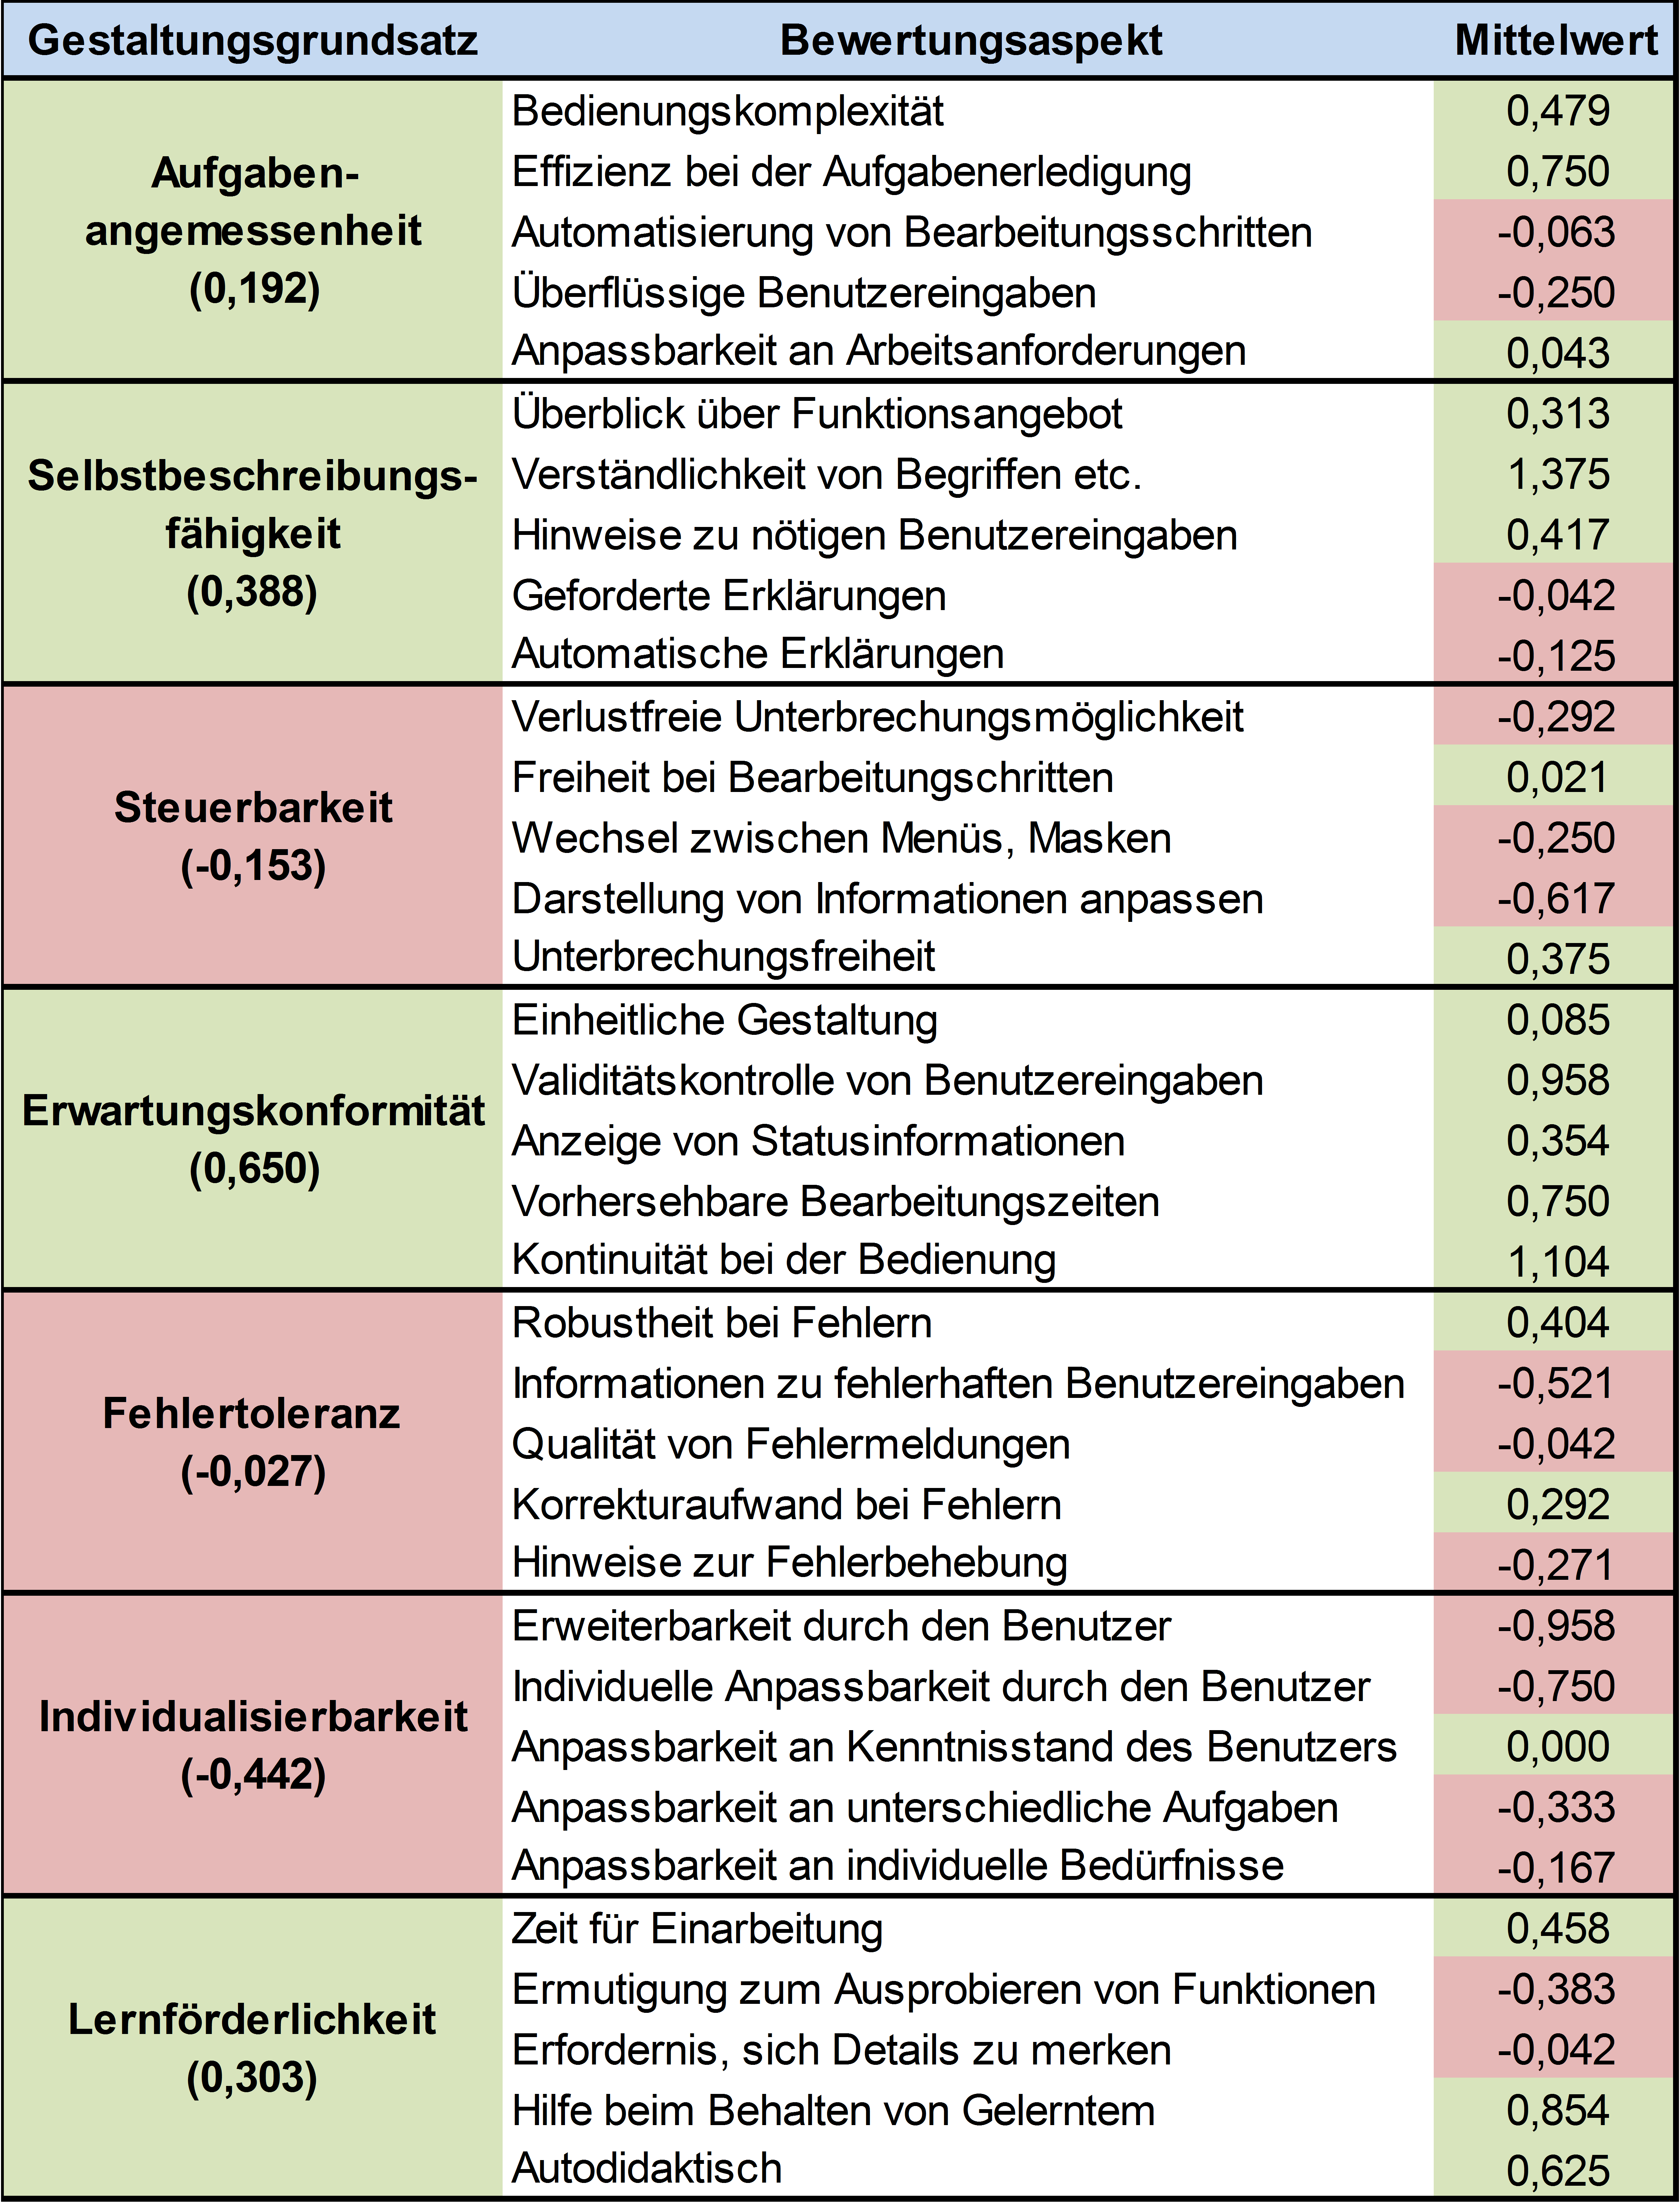
\includegraphics[width=430px]{img/Auswertungsmatrix_Alter_Dialog.PNG}
  \caption{Auswertungsmatrix zum ISO 9241-10 Fragebogen alter Dialog.}
  \caption*{\textbf{Quelle:} Eigene Darstellung}
  \label{fig:auswertungsmatrixAlterDialog}
\end{figure}
\end{minipage}

\anhang{Diagramme}
\subanhang{Ablauf Zwangsvollstreckung}
\label{sec:ablaufZwangsvollstreckung}
\begin{minipage}{\textwidth}
  \centering
  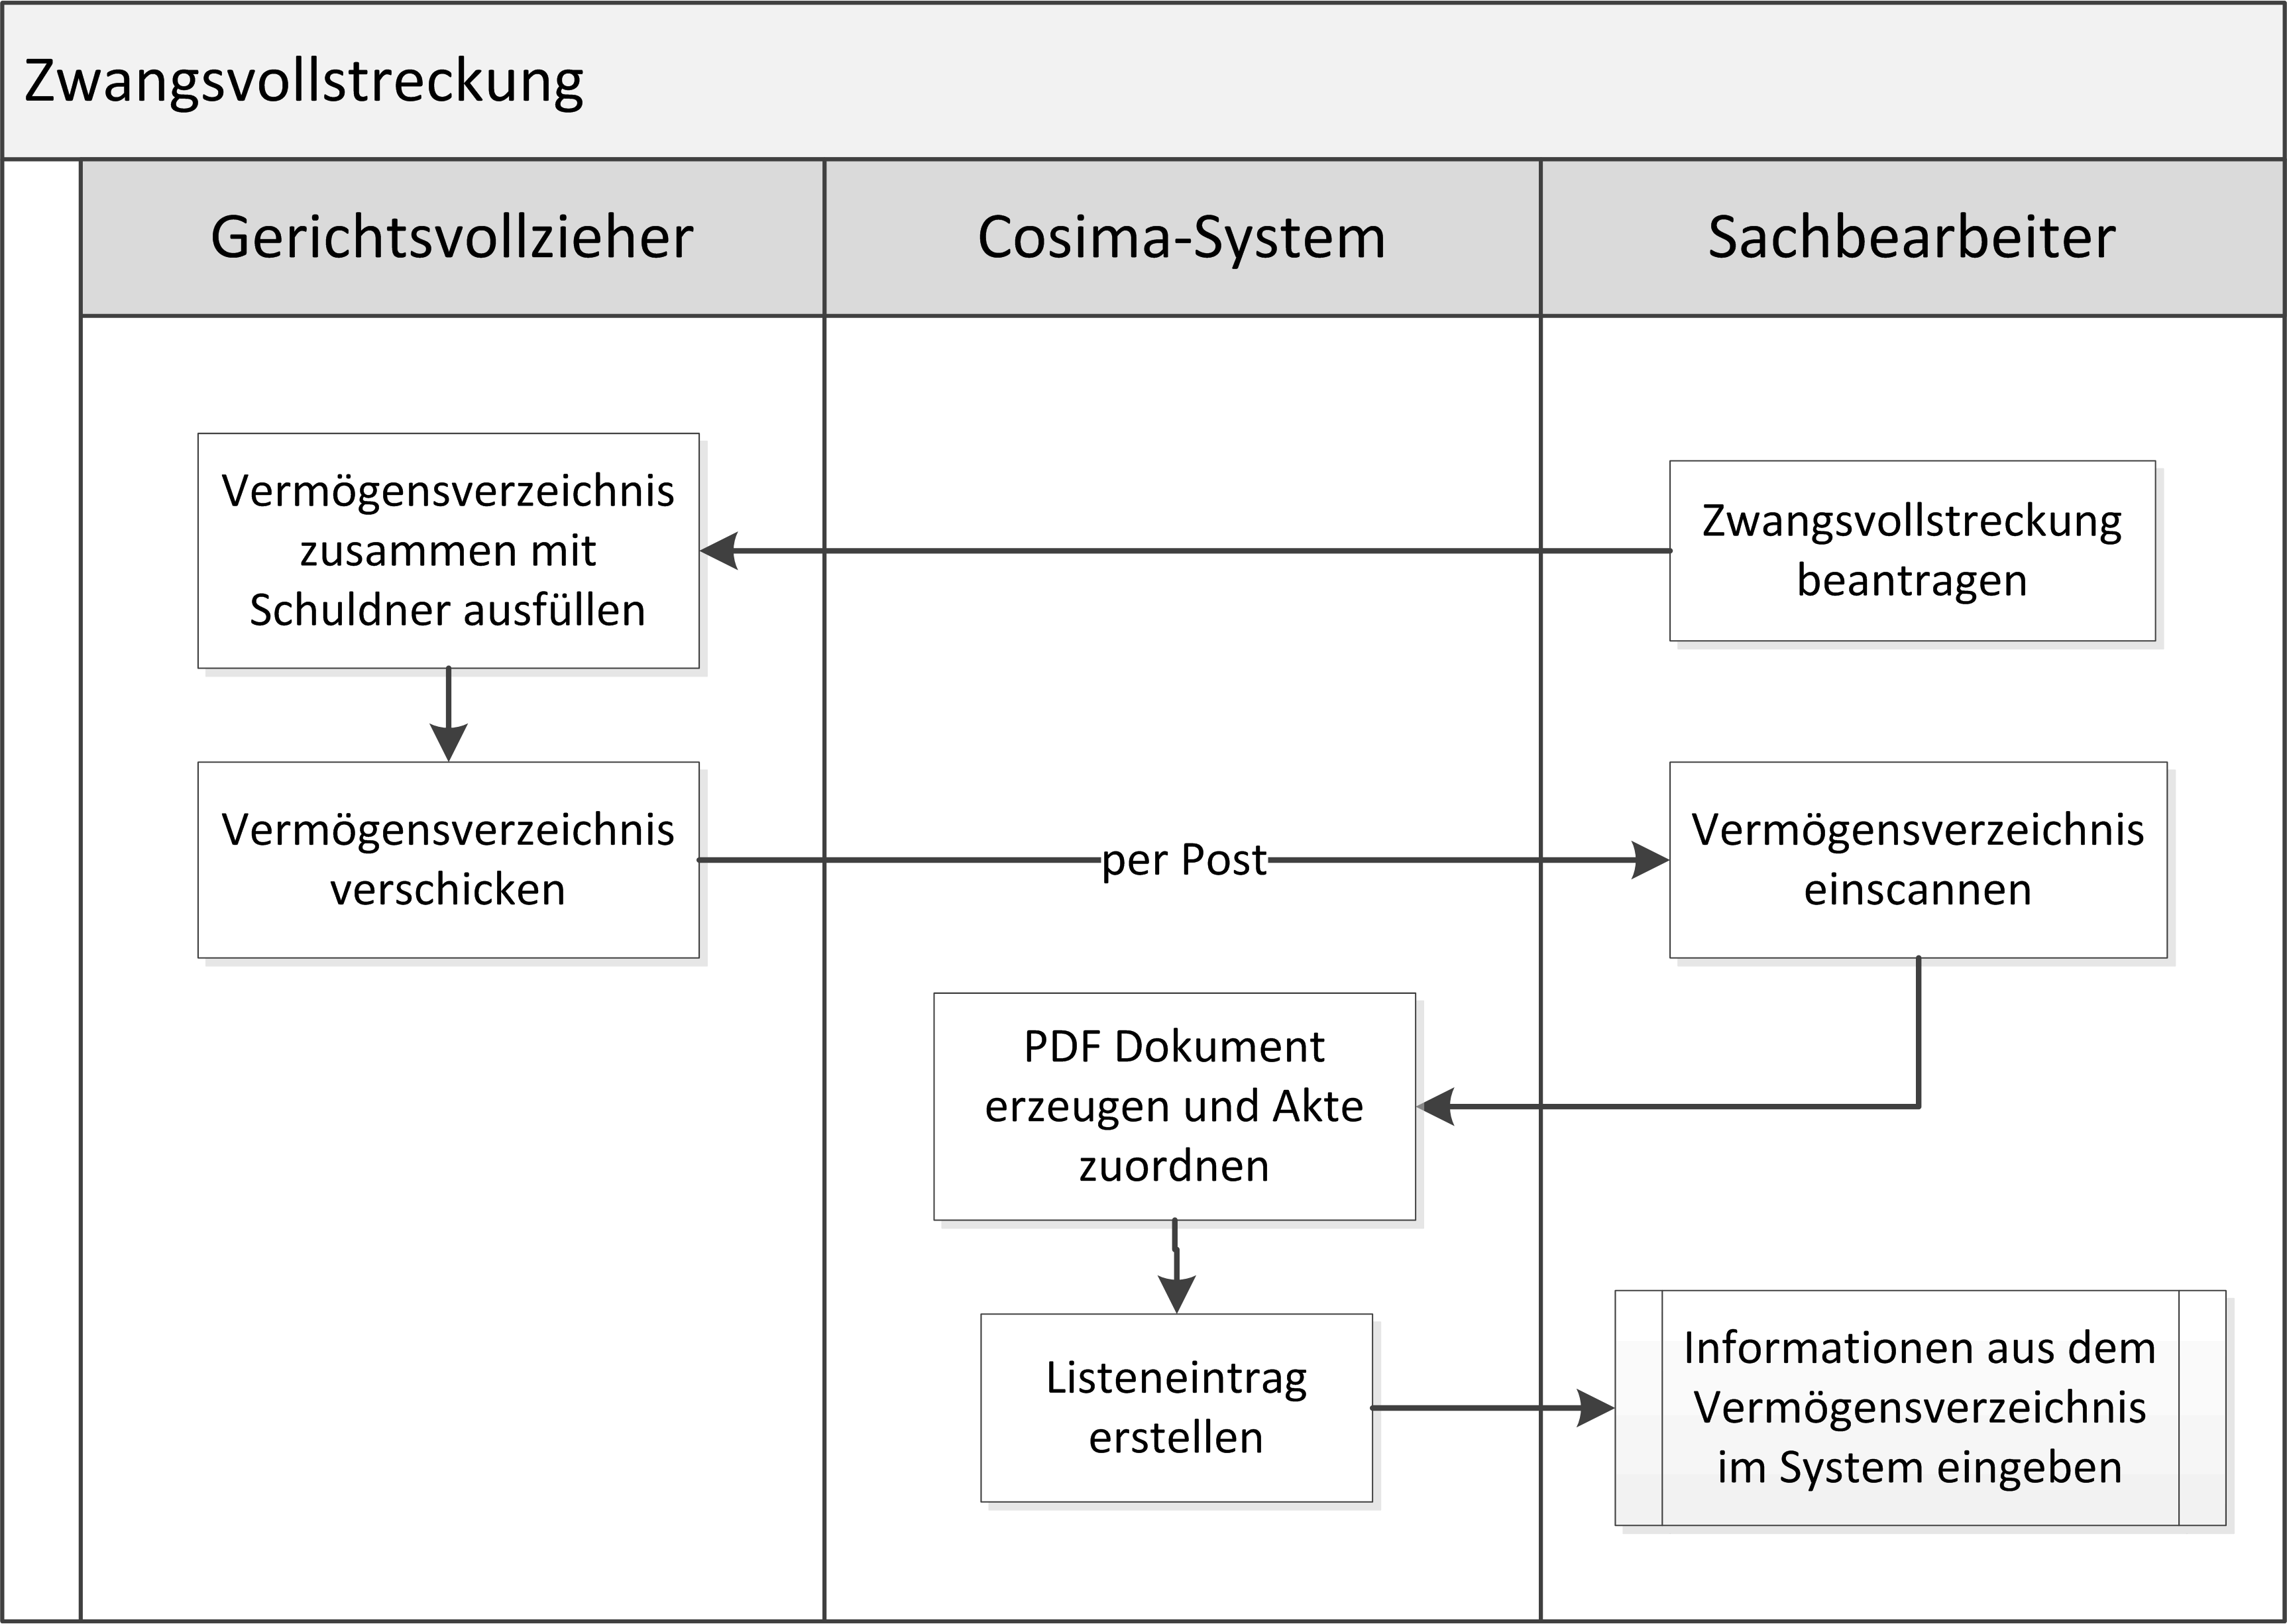
\includegraphics{img/Zwangsvollstreckung_Prozess.png}
  \captionof{figure}{Interaktion zwischen den Beteiligten bei der Zwangsvollstreckung.}
  \caption*{\textbf{Quelle:} Eigene Darstellung}
  \label{fig:zwangsvollstreckungProzess}
\end{minipage}

\subanhang{ERM UIDataCollector}
\label{sec:ermUIDataCollector}
\begin{minipage}{\textwidth}
  \centering
  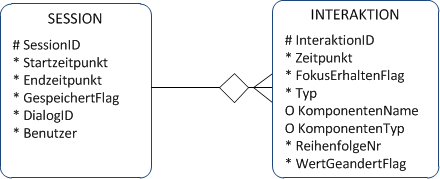
\includegraphics[scale=0.9]{img/ERM_UIDataCollector.PNG}
  \captionof{figure}{Entity Relationship Model des UIDataCollectors nach Barker Notation \citep[vgl.][]{Inguanez2012}}
  \caption*{\textbf{Quelle:} Eigene Darstellung}
  \label{fig:ermUIDataCollector}
\end{minipage}

\anhang{Dokumente}
\subanhang{Beispielformular Vermögensverzeichnis}
\label{sec:beispielVermoegensverzeichnisFormular}

\begin{minipage}{\textwidth}
  \centering
  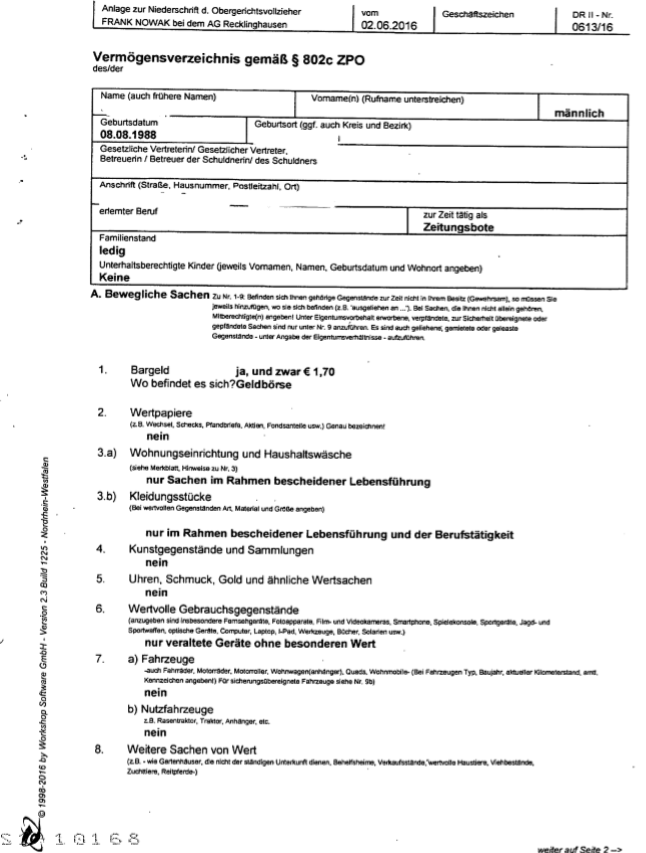
\includegraphics{img/VVformular_teil1.PNG}
\end{minipage}

\bigskip\noindent
\begin{minipage}{\textwidth}
  \centering
  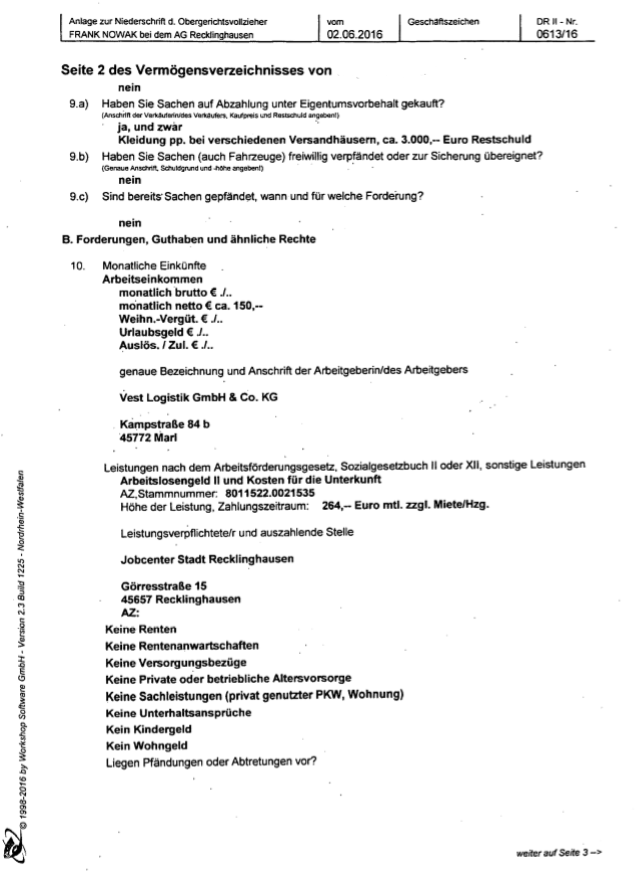
\includegraphics{img/VVformular_teil2.PNG}
\end{minipage}

\bigskip\noindent
\begin{minipage}{\textwidth}
  \centering
  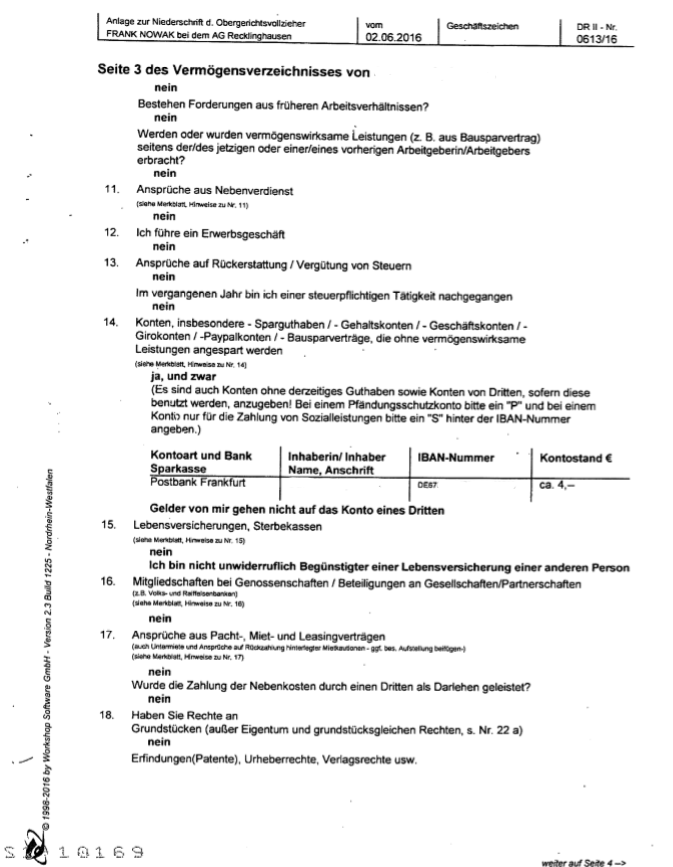
\includegraphics{img/VVformular_teil3.PNG}
\end{minipage}

\bigskip\noindent
\begin{minipage}{\textwidth}
  \centering
  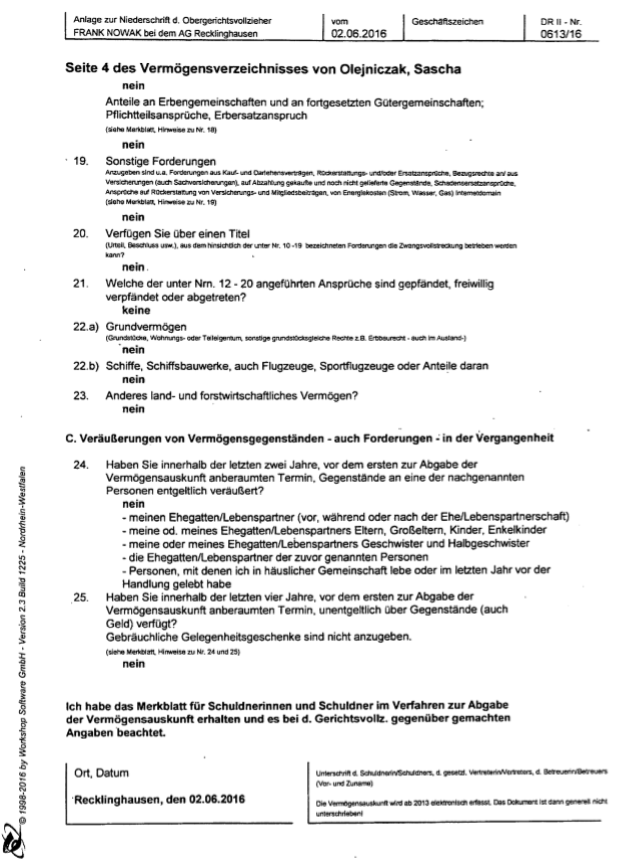
\includegraphics{img/VVformular_teil4.PNG}
\end{minipage}


\subanhang{ISO9241-10 Fragebogen}
\label{sec:ISOFragebogen}
\bigskip\noindent
\begin{minipage}{\textwidth}
  \centering
  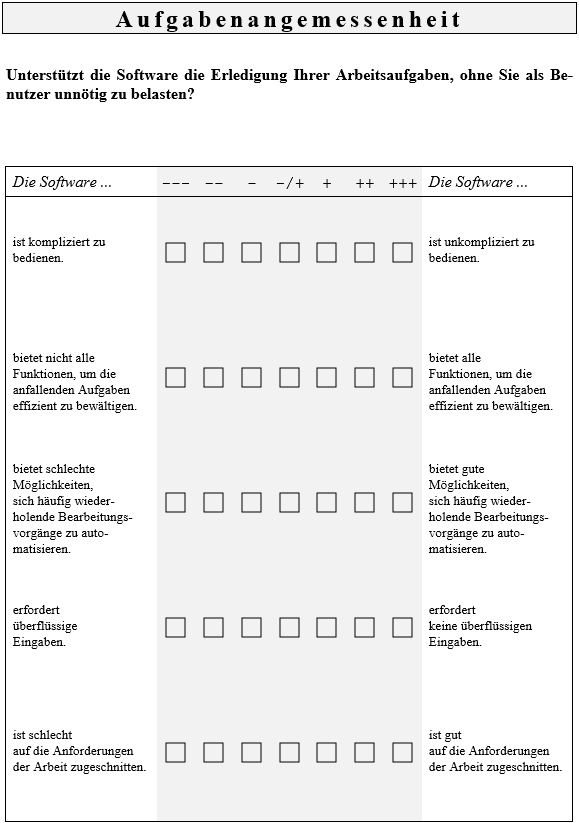
\includegraphics{img/ISO9241-10Fragebogen_S1.PNG}
\end{minipage}

\bigskip\noindent
\begin{minipage}{\textwidth}
  \centering
  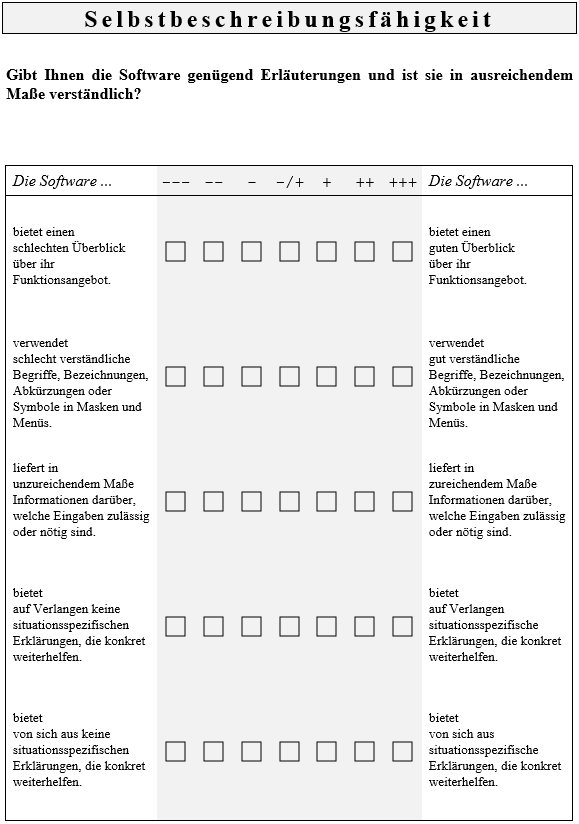
\includegraphics{img/ISO9241-10Fragebogen_S2.PNG}
\end{minipage}

\bigskip\noindent
\begin{minipage}{\textwidth}
  \centering
  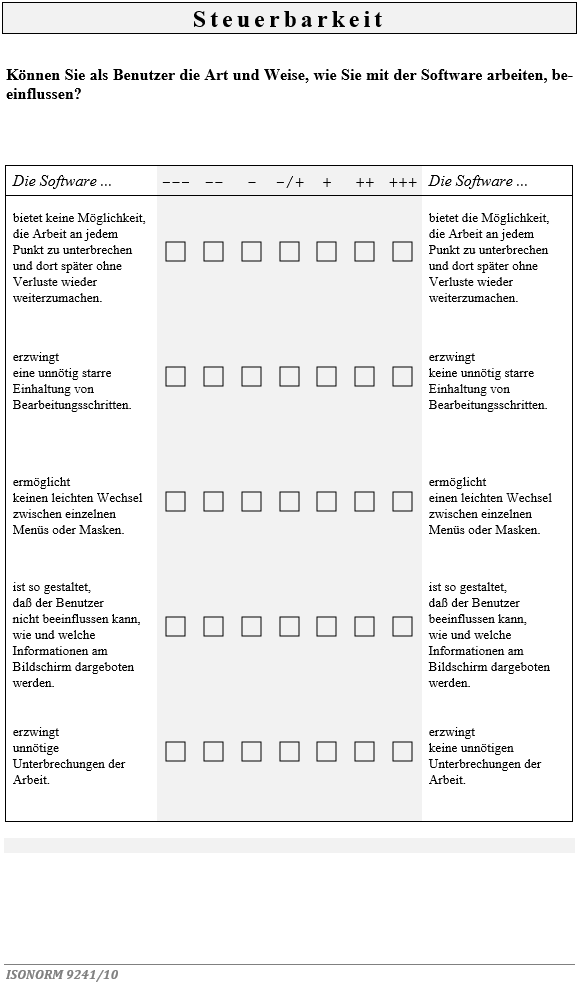
\includegraphics{img/ISO9241-10Fragebogen_S3.PNG}
\end{minipage}

\bigskip\noindent
\begin{minipage}{\textwidth}
  \centering
  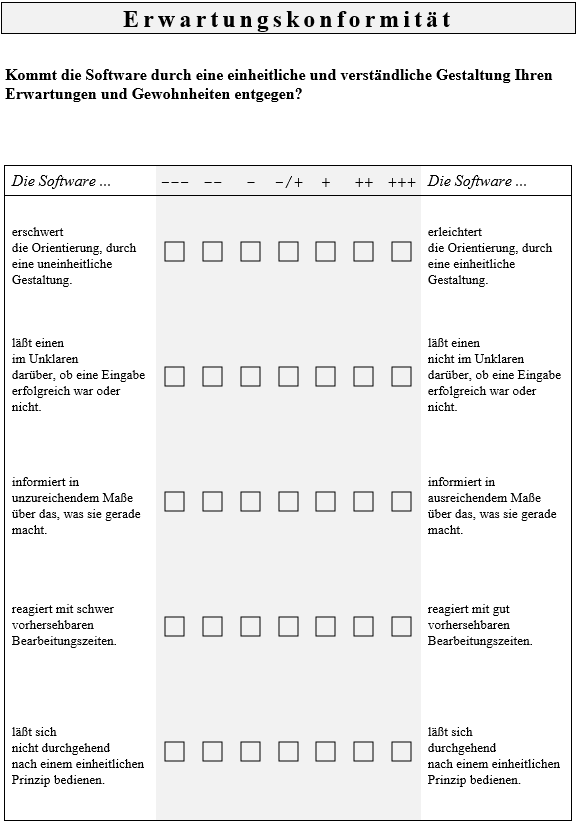
\includegraphics{img/ISO9241-10Fragebogen_S4.PNG}
\end{minipage}

\bigskip\noindent
\begin{minipage}{\textwidth}
  \centering
  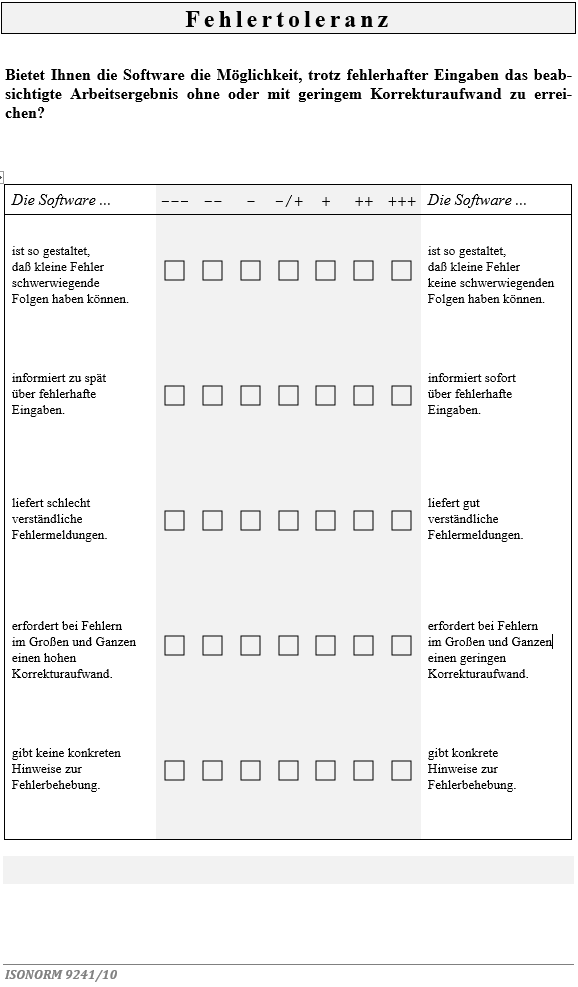
\includegraphics{img/ISO9241-10Fragebogen_S5.PNG}
\end{minipage}

\bigskip\noindent
\begin{minipage}{\textwidth}
  \centering
  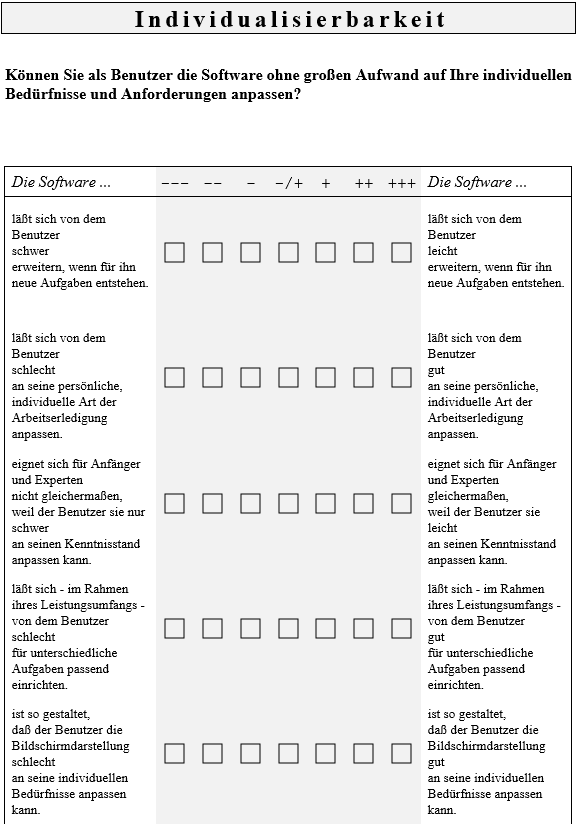
\includegraphics{img/ISO9241-10Fragebogen_S6.PNG}
\end{minipage}

\bigskip\noindent
\begin{minipage}{\textwidth}
  \centering
  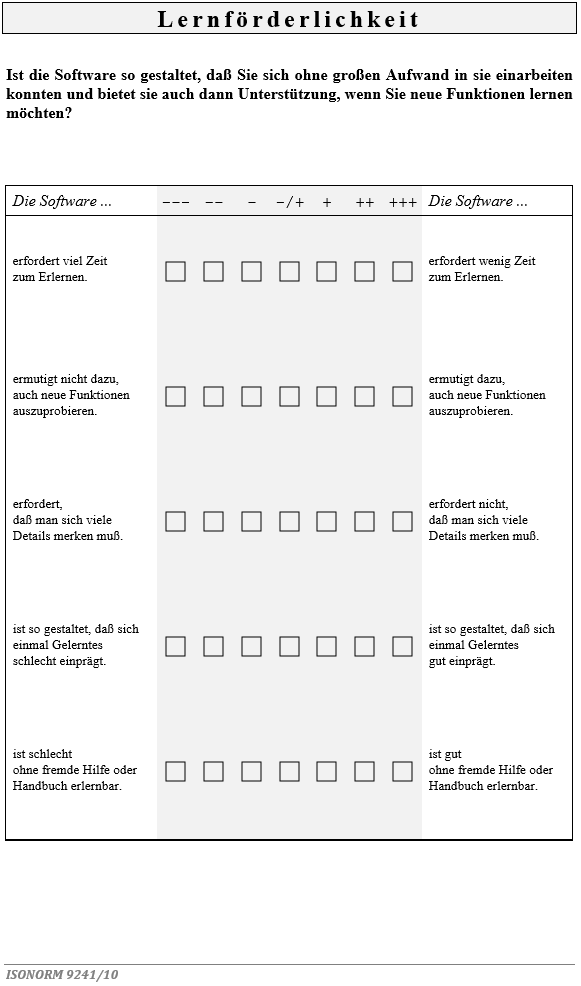
\includegraphics{img/ISO9241-10Fragebogen_S7.PNG}
\end{minipage}

%!TEX root = ../Thesis.tex
\section*{Quellenverzeichnis}
\addcontentsline{toc}{section}{Quellenverzeichnis}
\fancyhead[R]{Quellenverzeichnis}

\defbibheading{mono}{\subsection*{Monographien}}
\defbibheading{mag}{\subsection*{Aufsätze in Sammelbänden und Zeitschriften}}
\defbibheading{art}{\subsection*{Zeitungsartikel}}
\defbibheading{web}{\subsection*{Internetquellen}}
\defbibheading{leg}{\subsection*{Rechtsprechung}}
\defbibheading{lex}{\subsection*{Lexika und Enzyklopädien}}
\defbibheading{comp}{\subsection*{Unternehmensunterlagen/Gesprächsnotizen}}
\defbibheading{noge}{\subsection*{Normen und Gesetze}}

\setlength\bibitemsep{1.5\itemsep}
\setlength{\bibhang}{2em}

\renewcommand{\baselinestretch}{1.50}\normalsize

\begingroup
\sloppy

\printbibliography[heading=mono,keyword=mono]
\printbibliography[heading=mag,keyword=mag]
\printbibliography[heading=web,keyword=web]
\printbibliography[heading=lex,keyword=lex]
%\printbibliography[heading=art,keyword=art]
%\printbibliography[heading=leg,keyword=leg]
\printbibliography[heading=comp,keyword=comp]
\printbibliography[heading=noge,keyword=noge]

\endgroup


%%%%%%%%%%%%%%%%%%%%%%%%%%%%%%%%%%%%%%%%%%%%%%%%%%%%%%%%%%%%%%%%%%%%%%%

%!TEX root = ../Thesis.tex

\section*{Ehrenwörtliche Erklärung}
\addcontentsline{toc}{section}{Ehrenwörtliche Erklärung}
\fancyhead[R]{Ehrenwörtliche Erklärung}

Hiermit erkläre ich, dass ich die vorliegende \dokumententyp{} selbständig angefertigt habe. Es wurden nur die in der Arbeit ausdrücklich benannten Quellen und Hilfsmittel benutzt. Wörtlich oder sinngemäß übernommenes Gedankengut habe ich als solches kenntlich gemacht. Diese Arbeit hat in gleicher oder ähnlicher Form noch keiner Prüfungsbehörde vorgelegen.
\vspace{20mm}

\ort, \abgabedatum
\vspace{10mm}

\underline{\hspace{8cm}}\\\dokumentenautor
 
%%%%%%%%%%%%%%%%%%%%%%%%%%%%%%%%%%%%%%%%%%%%%%%%%%%%%%%%%%%%%%%%%%%%%%%

\end{document}